%
% Protocols for the Quantum Internet
%

\dropcap{T}{here} are countless applications for the long-distance communication and processing of quantum data. We will outline some of the most notable examples. Broadly, we will begin with discussion of \textit{low-level protocols} that form the primitives upon which other protocols are built. We will then progressively move towards \textit{high-level protocols}, culminating with full \textit{cloud quantum computing}.

Much of the recent experimental progress in quantum technology has been in the area of low-level protocols, although demonstrations of higher-level protocols are rapidly accelerating.

We keep in mind that although throughout this presentation we have been very quantum computing-centric, quantum computing is not the \textit{only} quantum resource worth communicating. In the same way that \textit{digital assets} encompass a broad range of digital systems and information, any aspect of a quantum system -- from a state, to an operation, storage, to a measurement, or anything else -- could be treated as a \textit{quantum asset}\index{Quantum assets}, which, for generality, we would like our quantum networks to be able to handle.

At the lowest physical level, quantum protocols have in common that they involve state preparation, evolution, and measurement as the fundamental primitives upon which more complex protocols are constructed. We consider these primitive resources in detail, before building upon them to consider some of the major elementary quantum protocols that implement tasks of practical interest. All of those discussed here have been subject to extensive experimental investigation and demonstration, which will be summarised in Sec.~\ref{sec:state_of_the_art}. We treat full quantum computation separately in Secs.~\ref{sec:models_QC} \& \ref{sec:archs_QC}, as this is such an involved topic in its own right.

We will employ circuit model diagrams when describing some protocols. The unfamiliar reader may refer to Sec.~\ref{sec:circuit_model} for a very brief introduction to quantum circuits.

Throughout this section the material will be optics-heavy, and not include discussion of some purely non-optical architectures, based on the reasonable assumption that networked quantum protocols will be optically mediated.

%
% State Preparation
%

\section{State preparation} \index{State preparation}

\dropcap{T}{he} first step in any quantum protocol involves the preparation of some kind of quantum state. Some quantum states are easy and cheap to prepare. Others are complex and costly. Thus, the most fundamental quantum asset that a quantum network must handle is the preparation and communication of quantum states.

A state prepared by Bob and sent to Alice might be prepared in isolation, or it might be entangled with a much larger system held by Charlie, that Alice does not have full access to. In that case, it would be impossible for Alice to prepare the state on her own, unless she were to first establish a relationship with Charlie. Alternately, maybe Alice just isn't very well-resourced, and can't do much on her own. The ability to let someone else prepare her desired quantum states for her would be highly appreciated.

Given the emphasis on quantum optics in quantum networking, it should be noted that optical quantum state engineering has broad applications, but can be very challenging in general. Single-photon state engineering, for example, finds ubiquitous applications in quantum information processing protocols, and has become commonplace. Most notably, linear optics quantum computing (Sec.~\ref{sec:KLM_univ}), and some quantum metrology protocols (Sec.~\ref{sec:metrology}) rely on single-photon state preparation. `Push-button' (i.e on-demand) single-photon sources would be a prized asset to many undergraduate experimentalists, were they able to afford them. But with access to the quantum internet, they could purchase single photons from another better-resourced lab, with QoS constraints guaranteed by QTCP.

The QTCP protocol is ideally suited to facilitating this kind of transaction. With the use of efficiency and purity cost metrics, QoS guarantees could be established for the efficiency and purity of a licensed single-photon source. In the case of single photons, the dephasing metric is irrelevant, since photon-number states are phase-invariant. This is an elegant example of the value of the versatility of having the QTCP protocol track multiple cost metrics for quantum packets, since different metrics will be of relevance to different messages. Were the message a coherent state, $\ket\alpha$, on the other hand, dephasing would be of utmost importance, whereas loss would be less critical, as lossy coherent states remain as coherent states and retain their coherence.

We see that even the most basic primitive in quantum technologies -- state preparation -- already brings with it much to take into consideration when designing quantum networks. However, the QTCP protocols we described earlier are versatile enough to be capable of mediating their distribution across quantum networks, whilst providing QoS guarantees.

%
% Coherent States
%

\subsection{Coherent states} \label{sec:coherent_states} \index{Coherent state preparation}

Coherent states (Sec.~\ref{sec:coherent_state_enc}), although not strictly \textit{quantum} states, nonetheless find broad applications in quantum protocols, for example as the pump for SPDC\index{Spontaneous parametric down-conversion (SPDC)} sources (Sec.~\ref{sec:single_phot_src}), or as a phase-reference\index{Phase-reference} for homodyne detection (Sec.~\ref{sec:homodyne})\index{Homodyne detection}. Coherent states are rather trivial to prepare, as they are closely approximated by laser sources. Despite their triviality, high quality lasers can nonetheless become very expensive, large, and inaccessible to the not-so-well-resourced end-user. It is not uncommon for laser sources in contemporary labs to be valued in the \$100k's.

%
% Single-Photons
%

\subsection{Single-photons} \label{sec:single_phot_src} \index{Single-photon state preparation}

Single-photon sources (Sec.~\ref{sec:single_phot_enc}) \cite{bib:Oxborrow05} are of particular interest, as a foundational building block in many optical quantum information processing applications, such as linear optics quantum computing (Sec.~\ref{sec:KLM_univ}) and quantum key distribution (Sec.~\ref{sec:QKD}).

The most common approach to preparing single-photon states is via heralded SPDC\index{Spontaneous parametric down-conversion (SPDC)} \cite{bib:URen03, bib:URen05}, whereby a coherent pump source is down-converted into two-mode photon-pairs via a second-order non-linear crystal with interaction Hamiltonian of the form,
\begin{align}
\hat{H}_\mathrm{SPDC} = \xi(\hat{a}_p\hat{a}_s^\dag\hat{a}_i^\dag + \hat{a}_p^\dag\hat{a}_s\hat{a}_i),
\end{align}
where $\xi$ is the interaction strength, and $\hat{a}_p$, $\hat{a}_s$ and $\hat{a}_i$ are the photonic annihilation operators for the pump (input), and \textit{signal} and \textit{idler} (output) modes respectively. This has the clear intuitive interpretation as the coherent exchange of photon-pairs in the output modes with photons in the coherent pump.

Specifically, a two-mode SPDC state takes the form,
\begin{align}
\ket\psi_\mathrm{SPDC} = \sqrt{1-\chi^2} \sum_{n=0}^\infty \chi^n \ket{n}_s\ket{n}_i,
\end{align}
where $\chi$ is the squeezing parameter, a function of the pump-power and properties of the crystal. The layout is shown in Fig.~\ref{fig:SPDC_source}.

\begin{figure}[!htbp]
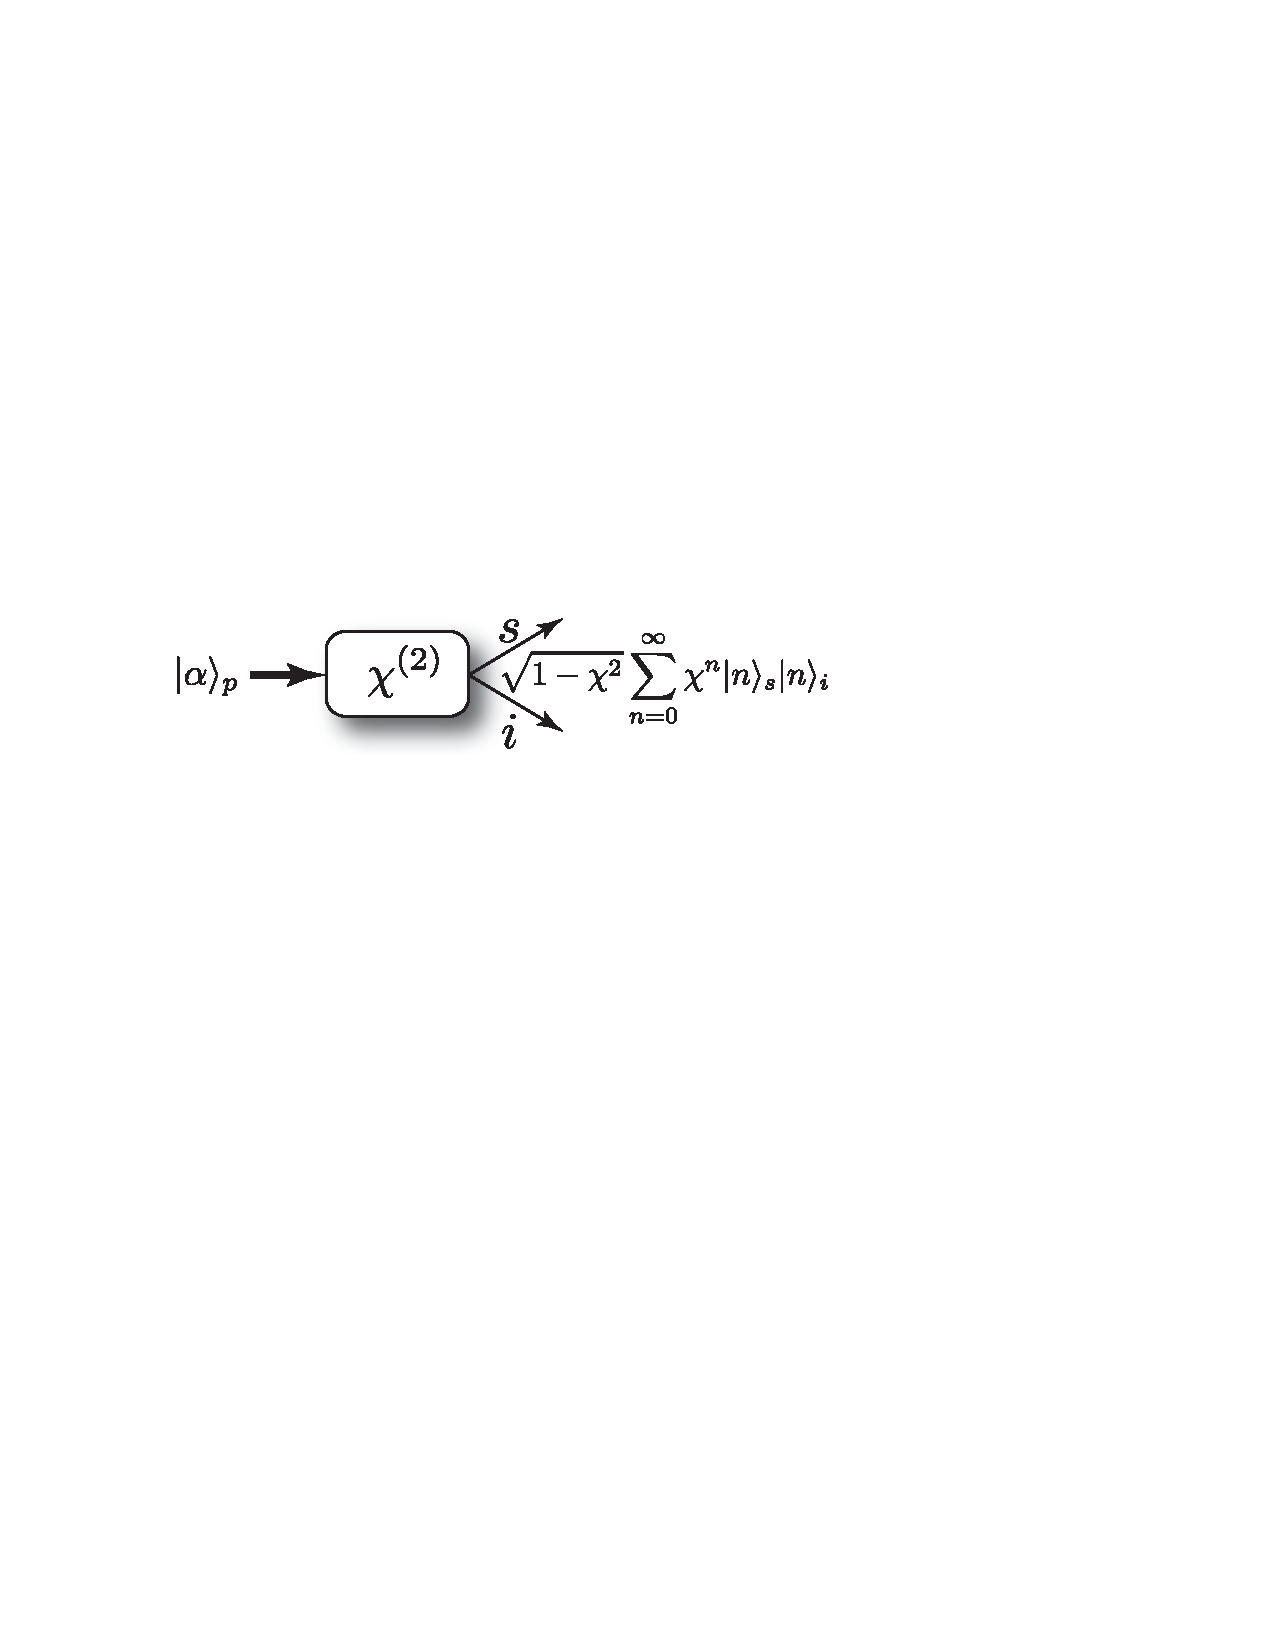
\includegraphics[clip=true, width=0.45\textwidth]{SPDC_source}
\captionspacefig \caption{Layout of an SPDC single-photon source. A second-order non-linear crystal is pumped with a coherent state (i.e laser source), yielding a two-mode output state with perfect photon-number correlation between the two modes. Then, post-selecting upon detecting a single photon in one mode in principle guarantees a single photon in the other.} \label{fig:SPDC_source}
\end{figure}

Applying the single-photon projector, \mbox{$\ket{1}\bra{1}$}, to the first mode yields the single-photon state in the other, up to normalisation, which reflects the inherent non-determinism. The preparation success probability is derived from the amplitude of the \mbox{$n=1$} term as,
\begin{align} \label{eq:SPDC_p_prep}
P_\mathrm{prep}=\chi^2(1-\chi^2),
\end{align}
assuming ideal photo-detection. Thus, the perfect photon-number correlation enables heralded preparation of states with exactly one photon in principle.

Transitioning from heralded state preparation to quasi-deterministic state preparation may then be achieved by operating a bank of such sources in parallel, and multiplexing their outputs, such that when all sources are triggered simultaneously, if any one succeeds, the respective single photon is routed to the desired output mode \cite{???}, as shown in Fig.~\ref{fig:SPDC_multiplexing_arch}.

\begin{figure}[!htbp]
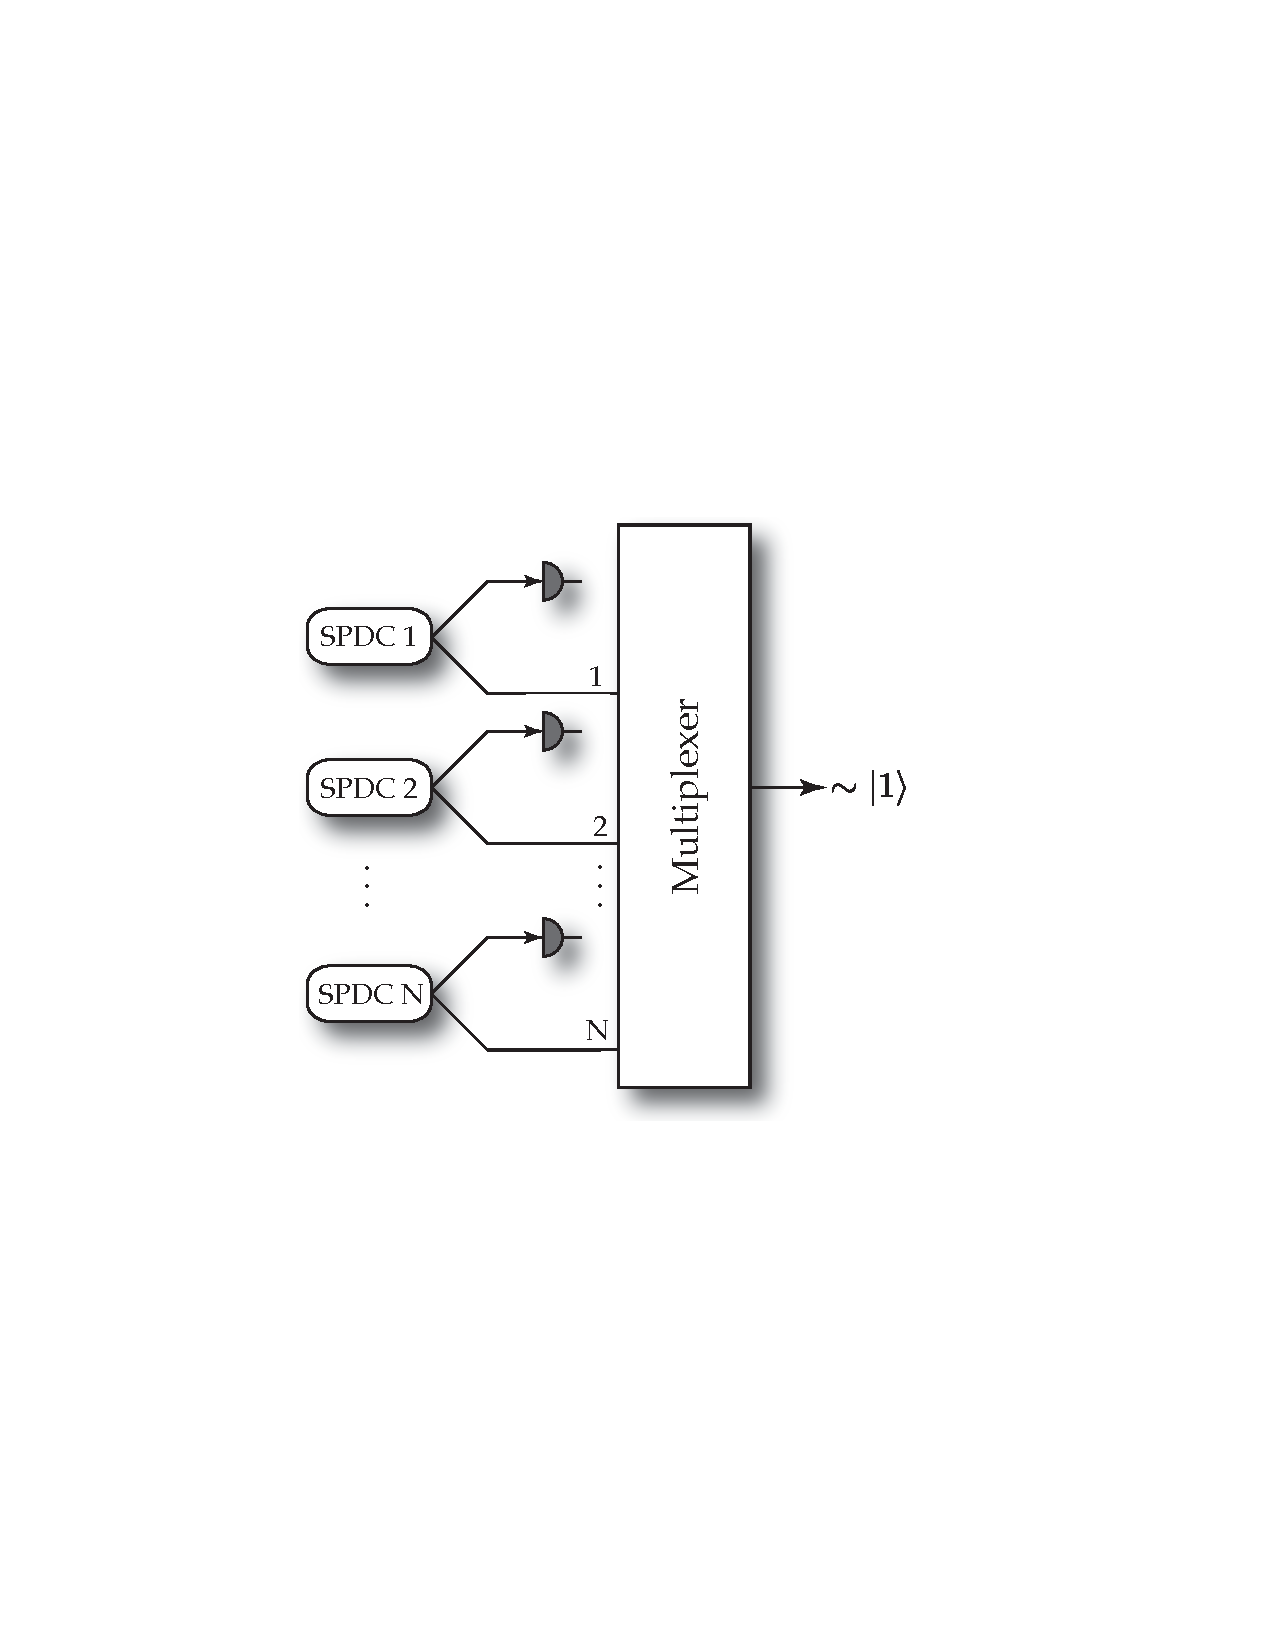
\includegraphics[clip=true, width=0.38\textwidth]{SPDC_multiplexing_arch}\index{Multiplexed single-photon sources}
\captionspacefig \caption{Quasi-deterministic single-photon state preparation using $N$-fold multiplexing of heralded SPDC sources (or any other non-deterministic, but heralded source). All $N$ SPDC sources are triggered simultaneously. The heralding detectors feedforward to the multiplexer, which routes a successfully heralded single-photon state (if there is one) to the output mode. With a sufficiently large bank of sources in parallel, the probability of successfully preparing a single-photon state approaches unity.} \label{fig:SPDC_multiplexing_arch}
\end{figure}

The success probability of the multiplexed source exponentially asymptotes to unity as the number of in-parallel sources increases,
\begin{align} \label{eq:SPDC_multiplex}
P_\mathrm{success} = 1 - (1-P_\mathrm{prep})^N,
\end{align}
where there are $N$ sources in parallel. This relationship is shown in Fig.~\ref{fig:SPDC_multiplexing_plot} for sources with varying heralding probabilities. This principle could also obviously be applied to any other type of non-deterministic, but heralded source.

\begin{figure}[!htbp]
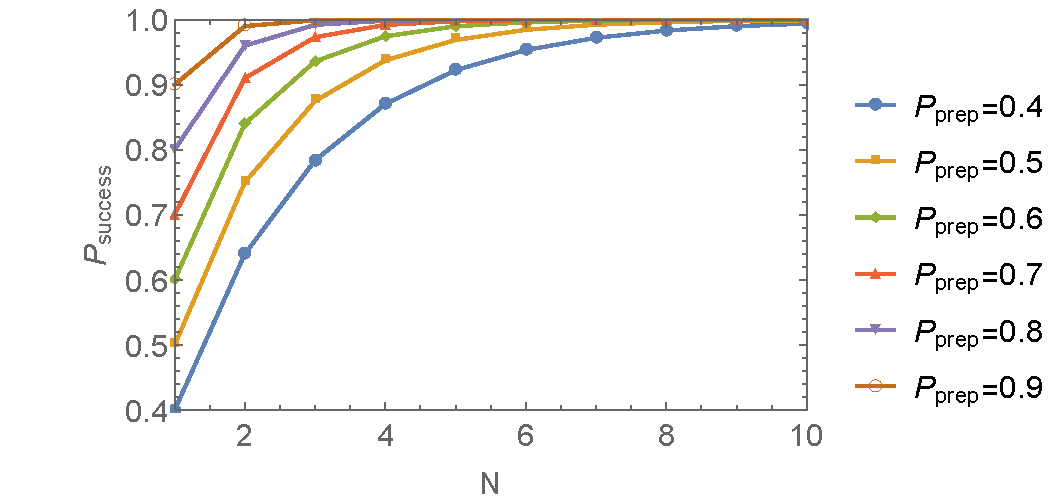
\includegraphics[clip=true, width=0.475\textwidth]{SPDC_multiplexing_plot}
\captionspacefig \caption{Single-photon state preparation probability, $P_\mathrm{success}$, using $N$-fold multiplexing, where the individual heralded sources have heralding probability $P_\mathrm{prep}$. $P_\mathrm{success}$ always exponentially asymptotes to unity with increasing $N$, for any \mbox{$P_\mathrm{prep}>0$}.} \label{fig:SPDC_multiplexing_plot}
\end{figure}

The multiplexing approach needn't be restricted to the spatial domain, but could also be equivalently implemented in the temporal domain \cite{bib:RohdeLoopMulti15, mosley, othersSeePaper}, as shown in Fig.~\ref{fig:SPDC_time_multiplexing}.

\begin{figure}[!htbp]
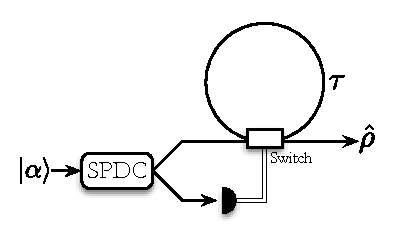
\includegraphics[clip=true, width=0.4\textwidth]{SPDC_time_multiplexing}
\captionspacefig \caption{Multiplexed single-photon state preparation in the temporal domain. An SPDC source operating at high repetition rate, with time-bin separation $\tau$, enters a fibre-loop with an in/out coupling switch classically controlled by the heralding outcomes. The fibre-loop acts as a quantum memory, keeping the most recent successfully heralded time-bin in memory until the procedure terminates. The output is a pulse-train where the last time-bin closely approximates a single-photon.} \label{fig:SPDC_time_multiplexing}
\end{figure}

Of course, operating a large bank of sources in parallel, along with the associated multiplexing, which requires nanosecond-scale fast-feedforward, is experimentally costly (both in physical size, complexity and dollars), making outsourcing of this technology potentially highly desirable.

This description is purely in the photon-number basis. However, as discussed in Sec.~\ref{sec:spatio_temporal}, photons also have spatio-temporal characteristics. This strongly affects state preparation when using heralded SPDC, particularly state purity, and much effort has been invested into engineering the spectral structure of SPDC states so as to maximise purity and indistinguishability \cite{bib:Aichele02, bib:Branning00}. Specifically, we wish to engineer the photon-pairs to be spectrally separable, such that the heralded photon remains spectrally pure even if the heralding photon was measured with undesirable spectral characteristics (e.g finite resolution).

SPDC is relatively cheap, and widely used, but nonetheless might be out of reach for many end-users, particularly when the previously discussed multiplexing techniques are employed to boost heralding efficiencies. It is quickly being superseded by superior technologies in cutting-edge labs, such as quantum dot sources, which have deterministic, push-button potential \cite{bib:Santori01, bib:Kiraz04}. Techniques based on cavity quantum electrodynamics (QED) \cite{bib:Brattke01} and molecular fluorescence \cite{bib:Brunel99} have also been demonstrated. However, such sources are very much in their developmental stages, and relatively expensive.

Generally speaking, a push-button photon source could be constructed from any two-level system, comprising a ground state, $\ket{g}$, and an excited state, $\ket{e}$, with short lifetime, whereby relaxation via the \mbox{$\ket{e}\to\ket{g}$} transition emits a photon. Then, pumping the system to excite it to the $\ket{e}$ state, and waiting for spontaneous decay yields a single photon.

%
% NOON States
%

\subsection{NOON states} \label{sec:NOON} \index{NOON state preparation}

So-called NOON states, path-number entangled two-mode states of the form,
\begin{align}
\ket\psi_\mathrm{NOON} = \frac{1}{\sqrt{2}}(\ket{N,0}+\ket{0,N}),
\end{align}
may be exploited to perform Heisenberg-limited quantum metrology\index{Quantum metrology} (Sec.~\ref{sec:metrology}), allowing extremely precise phase measurement with large photon-number $N$ \cite{bib:Dowling08}. 

The extreme sensitivity of NOON states owes to the $N$-fold enhancement in phase-dependence associated with the $N$-photon component of the superposition. Specifically, if a phase $\phi$ is present in only the second mode, the state evolves to,
\begin{align}
e^{i\phi\hat{n}} \ket\psi_\mathrm{NOON} = \frac{1}{\sqrt{2}}(\ket{N,0}+e^{i\phi N}\ket{0,N}),
\end{align}
where \mbox{$\hat{n}=\hat{a}^\dag\hat{a}$} is the photon-number operator associated with the second mode\index{Photon-number operator}. The phase enhancement arises because \mbox{$\hat{n}\ket{N}=N\ket{N}$}. Then, a simple interferometric procedure is able to extract this enhanced phase-dependence as an observable.

However, these states are notoriously difficult and technologically challenging to prepare, and can only be prepared non-deterministically using linear optics \cite{bib:Cable07, bib:PhysRevA.65.030101, bib:PhysRevA.76.063808}. If a remote server had the capacity to prepare such states, they would be in high demand across the globe. Hindering this, NOON states are very fragile creatures. First, they exhibit exponentially increased susceptibility to loss -- loss of just a single photon completely decoheres the state, rendering it useless for metrological purposes. Second, the large photon-number, $N$, amplifies unwanted dephasing by a factor of $N$, as discussed in Sec.~\ref{sec:dephasing_error}. These considerations can be readily accommodated for in the QTCP protocol by tracking dephasing and loss metrics of the packets encapsulating the NOON states.

%
% Cluster States
%

\subsection{Cluster states} \index{Cluster state preparation}

In addition to the simple single- or two-mode states discussed above, an entire universal quantum computation can be performed using the `cluster state' measurement-based model for quantum computation (explained in detail in Sec.~\ref{sec:CSQC}). Here state preparation can not only be outsourced, but distributed, with different hosts preparing different geometric parts of the state, which are then `stitched together'.

The beauty of this type of state is that there is a natural separation between state preparation and computation, with the preparation stage being far more technologically challenging than the computation stage. Thus, Alice might ask better-resourced Bob to prepare a cluster state and send it to her, at which point she implements the computation herself using only simple single-qubit measurement operations.

A detailed discussion of optical cluster state preparation is presented in Sec.~\ref{sec:CS_LO}, with a focus on protocols employing non-deterministic gates.

%
% Greenberger-Horne-Zeilinger States
%

\subsection{Greenberger-Horne-Zeilinger states} \index{Greenberger-Horne-Zeilinger (GHZ) states}\label{sec:GHZ_states}

Another class of states is Greenberger-Horne-Zeilinger (GHZ) states \cite{bib:GHZ89}, which are maximally-entangled states across an arbitrary number of qubits, $n$, of the form,
\begin{align}
\ket\psi_\mathrm{GHZ}^{(n)} = \frac{1}{\sqrt{2}}(\ket{0}^{\otimes n} + \ket{1}^{\otimes n}).
\end{align}

GHZ states are useful for various quantum information processing applications, including quantum anonymous broadcasting (Sec.~\ref{sec:anon_broad}). These states are particularly susceptible to loss, since the loss of a single qubit completely decoheres the state into a perfect mixture of the \mbox{$\ket{0}^{\otimes (n-1)}$} and \mbox{$\ket{1}^{\otimes (n-1)}$} states, with complete loss of entanglement and coherence,
\begin{align}
\hat\rho_\mathrm{GHZ}^\mathrm{loss} &= \mathrm{tr}_1(\ket\psi_\mathrm{GHZ}^{(n)}\bra\psi_\mathrm{GHZ}^{(n)})\nonumber \\
&= \frac{1}{2}(\ket{0}^{\otimes (n-1)}\bra{0}^{\otimes (n-1)}+\ket{1}^{\otimes (n-1)}\bra{1}^{\otimes (n-1)}).
\end{align}

A simple linear optics circuit for the preparation of 3-qubit polarisation-encoded GHZ states is shown in Fig.~\ref{fig:GHZ_LO_prep}.

\begin{figure}[!htbp]
	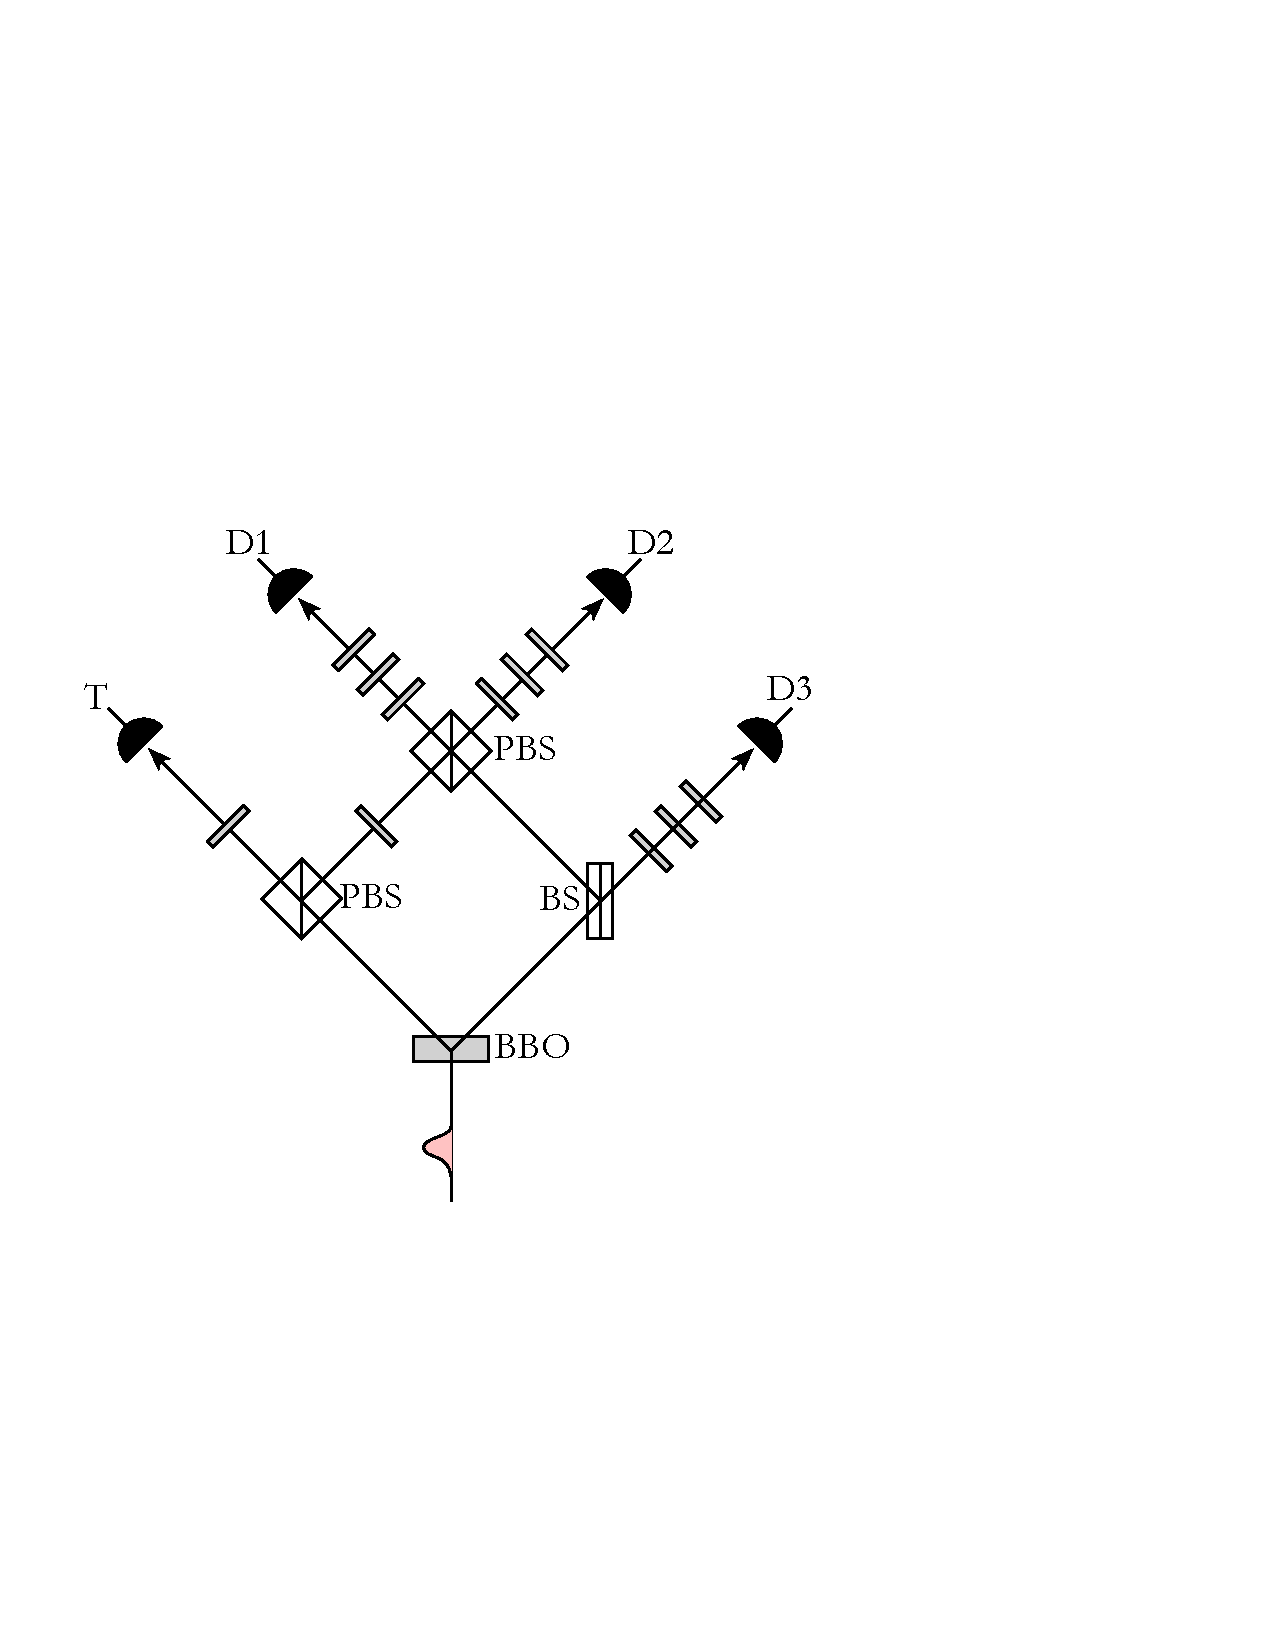
\includegraphics[clip=true, width=0.475\textwidth]{GHZ_LO_prep}
	\captionspacefig \caption{Linear optics circuit for the non-deterministic preparation of 3-qubit polarisation-encoded GHZ states \cite{ZeilingerPan}. A BBO SPDC source is pumped into the double excitation regime. Following evolution through the linear optics network, measurement of a photon in the tigger mode ($T$) heralds the preparation of a GHZ state across modes $D1$, $D2$ and $D3$.}\label{fig:GHZ_LO_prep}
\end{figure}

%
% W-states
%

\subsection{W-states}\index{W-states}\label{sec:W_state_prep}

W-states are a class of non-maximally-entangled states across an arbitrary number of qubits/modes. They are given by the equal superposition of a single excitation/`1' across all $n$ qubits. Thus, there are $n$ terms in the superposition, of the form,
\begin{align}
\ket\psi_\mathrm{W}^{(n)} &= \frac{1}{\sqrt{n}} \sum_{i=1}^n \hat{a}_i^\dag \ket{0}^{\otimes n}\nonumber\\
&= \frac{1}{\sqrt{n}}(\ket{1,0,0,0,\dots} + \ket{0,1,0,0,\dots}\nonumber\\
&+ \ket{0,0,1,0,\dots} + \ket{0,0,0,1,\dots} + \dots).
\end{align}

W-states are a class of states distinct from GHZ states (for any \mbox{$n\geq 3$}). Unlike GHZ states, W-states preserve some entanglement when a single qubit is traced out of the system, giving them a degree of robustness against qubit loss. This property is discussed in further detail in Secs.~\ref{sec:atomic_ens} \& \ref{sec:error_averaging}, where this property is exploited for error correction purposes.

Using linear optics, W-states are amongst the most trivial entangled states to prepare, using a simple fanout operation. An $n$-mode W-state can be prepared directly using $n$ beamsplitters in a linear cascade, as shown in Fig.~\ref{fig:W_state_LO_prep}(a), where the beamsplitter reflectivities are chosen so as to create the uniform superposition, given by the pattern,
\begin{align}
	{\eta_1}^2 &= 1 - \frac{1}{n},\nonumber\\
	{\eta_1}^2 {\eta_2}^2 &= \frac{1}{n},\nonumber\\
	{\eta_1}^2 {\eta_3}^2 (1-{\eta_2}^2)  &= \frac{1}{n},\nonumber\\
	{\eta_1}^2 {\eta_4}^2(1-{\eta_2}^2) (1-{\eta_3}^2)  &= \frac{1}{n},\nonumber\\
	{\eta_1}^2 {\eta_i}^2 \prod_{j=2}^{i-1} (1-{\eta_j}^2) &= \frac{1}{n},\nonumber\\
	{\eta_n}^2 &= 1.
\end{align}
Alternately, they can be made from a pyramid fanout network of \mbox{$\eta=1/\sqrt{2}$} beamsplitters, as shown in Fig.~\ref{fig:W_state_LO_prep}(b).

\begin{figure}[!htb]
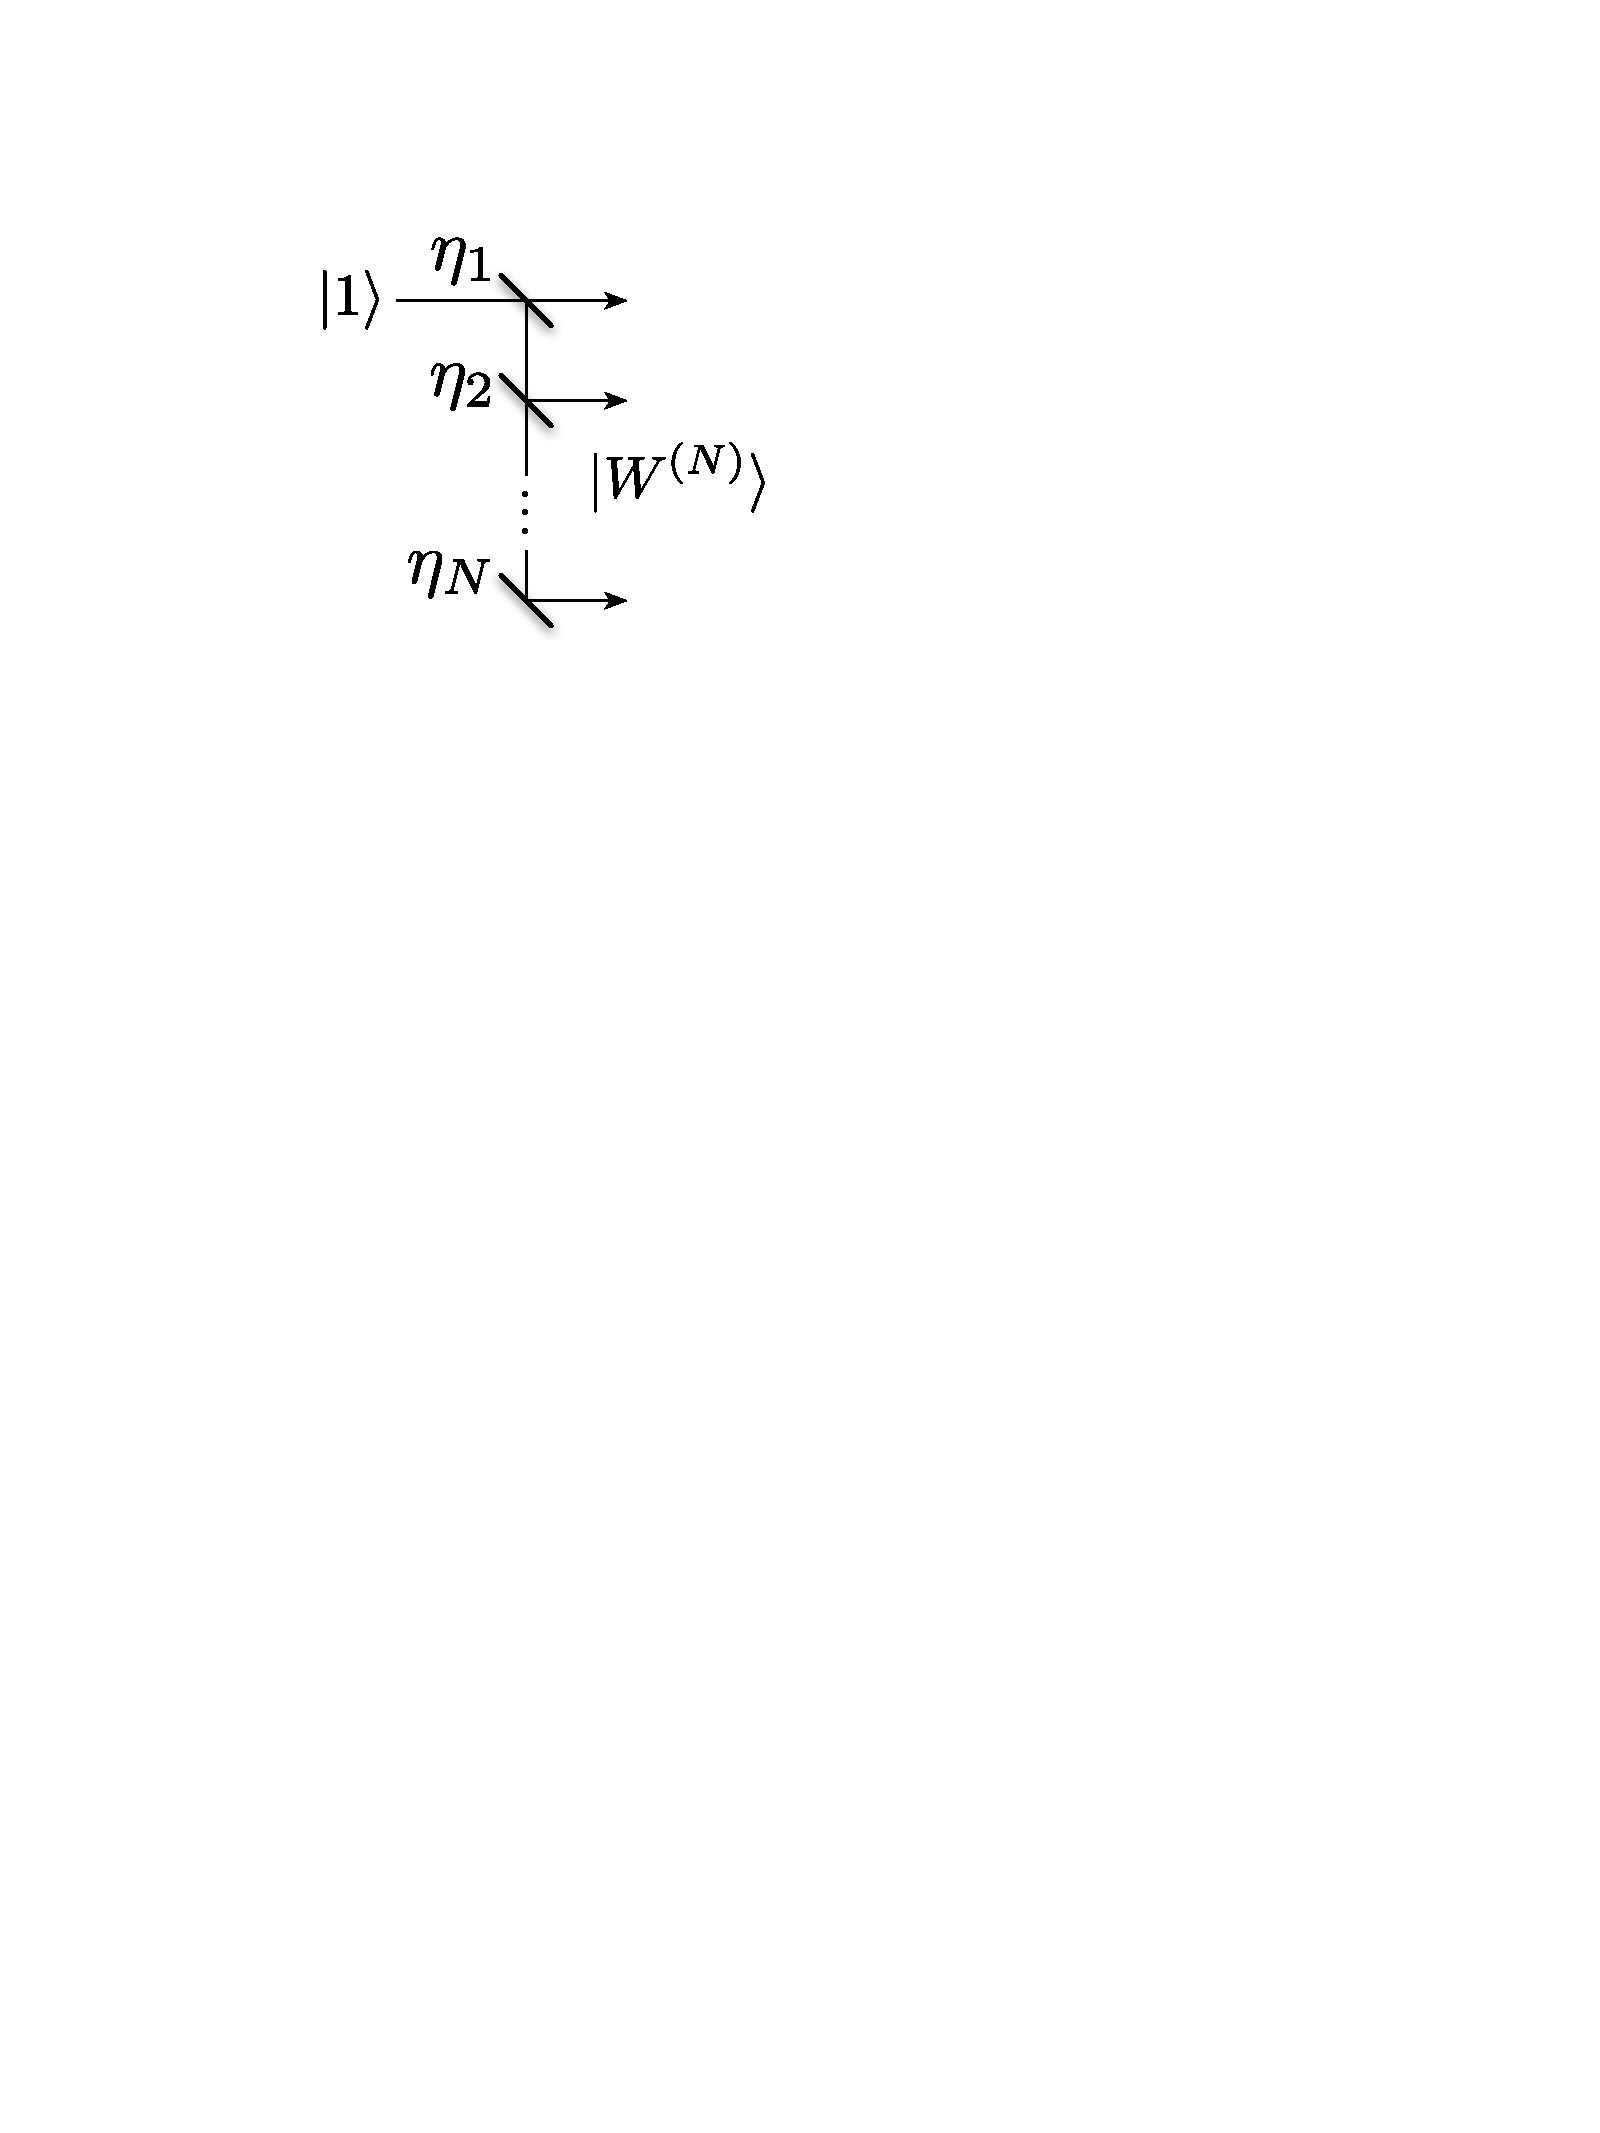
\includegraphics[clip=true, width=0.475\textwidth]{W_state_LO_prep}
\captionspacefig \caption{Preparation of an $n$-mode W-state using a single-photon source and a (a) linear cascade of beamsplitters, (b) a pyramid network of beamsplitters. The latter has the advantage that paths are balanced, in the sense that all routes pass through the same number of optical elements. Additionally the pyramid network has only \mbox{$O(\log n)$} depth, compared to the worst-case \mbox{$O(n)$} depth of the linear cascade. This is a relevant consideration when optical elements are lossy or induce errors.}\label{fig:W_state_LO_prep}	
\end{figure}

More generally, an entire basis of W-states\footnote{We refer to a `basis' of W-states as being a set of states that are all equivalent to a standard W-state up to local phases.} is accessible using linear optics networks described by unitaries where all matrix elements have amplitude $1/\sqrt{n}$, differing only via local phases. This includes the generalised Hadamard transform\index{Hadamard transform}, and quantum Fourier transform\index{Quantum Fourier transform}.

%
% Bell States
%

\subsection{Bell states} \label{sec:bell_state_res} \index{Bell state preparation}

Bell states, also known as Einstein-Podolsky-Rosen (EPR) pairs\index{Bell states} \cite{bib:EPR35}, which are maximally-entangled 2-qubit states, are particularly useful for many applications, including quantum teleportation (Sec.~\ref{sec:teleport}), cluster state preparation (Sec.~\ref{sec:CSQC}), and entanglement swapping (Sec.~\ref{sec:swapping}). Bell states are the special case of 2-qubit cluster states, or equivalently, 2-qubit GHZ states,
\begin{align}
	\ket{\Phi^+} = \ket\psi_\mathrm{GHZ}^{(2)}.
\end{align}

Bell pairs may be directly prepared as the two-mode output from a type-II\footnote{In type-II SPDC the photon-pair is polarisation-entangled, directly preparing a Bell pair in the polarisation basis. In type-I SPDC both photons have the same polarisation, yielding only photon-number correlation, but no polarisation entanglement.} SPDC source, or using non-deterministic linear optics from single-photon sources.

There are four Bell states\footnote{$\ket{\Psi^-}$ is also referred to as a \textit{singlet} state, and $\ket{\Psi^+}$ as a \textit{triplet} state.}, defined as, 
\begin{align} \label{eq:bell_basis}
\ket{\Phi^{\pm}} &= \frac{1}{\sqrt{2}} (\ket{0}_A\ket{0}_B \pm \ket{1}_A\ket{1}_B), \nonumber \\
\ket{\Psi^{\pm}} &= \frac{1}{\sqrt{2}} (\ket{0}_A\ket{1}_B \pm \ket{1}_A\ket{0}_B),
\end{align}
which are locally equivalent to one another via the application of Pauli operators, and may therefore be transformed to one another without classical or quantum communication between the two parties. Specifically,
\begin{align}
\ket{\Phi^+} = \hat{Z}\ket{\Phi^-} = \hat{X}\ket{\Psi^+} = \hat{X}\hat{Z}\ket{\Psi^-},
\end{align}
where $\hat{X}$ and $\hat{Z}$ could apply to either qubit, up to global phase. 

In Sec.~\ref{sec:ent_ultimate} we present the case that these states are so useful on their own that one might be justified in building entire quantum networks based purely upon the distribution of Bell pairs. This is the basis for \textit{quantum repeater networks}, which will be discussed in Sec.~\ref{sec:rep_net}.

%
% Cat States
%

\subsection{Cat states} \index{Cat state preparation}

Cat states (Sec.~\ref{sec:cat_enc}) -- superpositions of coherent states -- are extremely difficult to prepare, most easily via non-linear processes. However, they are very useful for optical quantum computation and for the study of macroscopic quantum systems, when using large coherent amplitudes. Because of the difficulty of their preparation, the ability to outsource it would be very valuable.

However, it must be cautioned that cat states decohere very readily, since their well-defined parity implies decoherence upon loss or measurement of just a single photon. This makes QoS considerations particularly pertinent.

%
% Squeezed States
%

\subsection{Squeezed states} \label{sec:squeezed} \index{Squeezed state preparation}

Of particular interest to metrology\index{Quantum metrology} and CV quantum computing\index{Continuous-variable quantum computation} in particular, are squeezed states, states which have been longitudinally distorted in phase-space. In the metrological context, squeezed states enable sub-shotnoise limited metrology \cite{???}, thereby outperforming any classical protocol, using, for example, coherent states.

Mathematically, squeezing is represented using the squeezing operator,
\begin{align}
\hat{S}(\xi) = \exp \left[ \frac{1}{2}(\xi^*\hat{a}^2 - \xi{\hat{a}^{\dag 2}})\right],
\end{align}
where $\hat{a}$ is the photonic creation operator, and $\xi$ is the squeezing parameter. Experimentally, such states are prepared using non-linear crystals. It is intuitively obvious that linear optics alone cannot prepare such states, owing to the non-linear terms in the squeezing operator, which do not preserve photon-number, and therefore cannot be passive.

Of particular interest are squeezed coherent states, $\hat{S}(\xi) \ket{\alpha}$, which are minimum uncertainty states, saturating the Heisenberg uncertainty relation. A special case of this is squeezed vacuum states, $\hat{S}(\xi) \ket{0}$, which are even-parity states (i.e containing strictly even photon-number terms). This implies that, like cat states, they are very vulnerable to decoherence for the same reason.

%
% More Exotic States of Light
%

\subsection{More exotic states of light}

As discussed in Sec.~\ref{sec:exotic}, many other far more elaborate states are very difficult to prepare, and it would be highly desirable if they could be obtained/purchased over a quantum network. This includes certain CV states, which have utility in alternate models for quantum computing \cite{bib:Menicucci06, Ralph, Lund}.

\comment{To do!}

\comment{Add hyperlinks to other relevant sections}

%
% Matter Qubits
%

\subsection{Matter qubits} \index{Matter qubits}

In addition to preparing optical states, they can be used to mediate the preparation of systems comprising matter qubits, using which-path erasure techniques (Sec.~\ref{sec:hybrid} \& Fig.~\ref{fig:barrett_kok}) or light-matter interactions (Sec.~\ref{sec:opt_inter} \& Fig.~\ref{fig:opt_int}). These techniques are very versatile, and apply to many different matter qubit systems, such as two-level atoms, nitrogen-vacancy centres, quantum dots, and atomic ensembles.

This is useful when matter-based architectures are more scalable or technologically simpler than all-optical architectures (Sec.~\ref{sec:KLM_univ}), and particularly for quantum memory (Sec.~\ref{sec:memory}), when using matter qubits with long lifetimes.

%
% Measurement
%

\section{Measurement} \index{Measurement}

\dropcap{A}{s} a last (and possibility also intermediate) step in any quantum protocol is the measurement of quantum states. State measurement is, in the most general context, essentially state preparation in reverse, and brings with it many of the same challenges.

Different detection schemes bring with them their own (potentially substantial) costs and technological challenges. State of the art micro-pillar photo-detectors\index{Micro-pillar photo-detectors} \cite{???}, at the time of writing, cost on the order of \$100k's, and require a sophisticated laboratory setup. Clearly this type of infrastructure is inaccessible to many players, and borrowing or licensing access to such equipment over a quantum network would pave the way for broader accessibility to state of the art technology.

Each type of state being measured, in combination with the nature of the detection scheme, brings with it their own limitations. Specifications of interest include dead-time, speed (relevant when implementing feedforward), and spatio-spectral filtering characteristics.

These represent significant technological challenges, which are costly to overcome, necessitating outsourcing over the quantum internet to become economically viable on a large scale. However, the QTCP protocol is able to accommodate error metrics and attributes covering all the above error models, enabling reliable, predictable QoS for outsourced quantum measurement.

With the ability to perform measurements over a complete basis for the respective system, QST, and consequently QPT (Sec.~\ref{sec:QPT}), can also be outsourced, as both these protocols are built entirely upon determining measurement expectation values in some known basis.

%
% Photo-detection
%

\subsection{Photo-detection} \label{sec:photo_detection} \index{Photo-detection}

Perhaps the most useful, and ubiquitous, type of optical state measurement is photo-detection \cite{bib:RohdePDReview}, where we would like to count photon-number. Broadly, there are two main classes of photo-detectors -- \textit{number-resolved}\index{Number-resolved photo-detectors} and \textit{non-number-resolved}\index{Non-number-resolved photo-detectors} (or `bucket' detectors). These behave exactly as the names suggest, with the former typically being more expensive and technologically demanding than the latter.

%
% Mathematical Representation
%

\subsubsection{Mathematical representation}

A completely general detector can be modelled as a POVM\index{POVM},
\begin{align}
\hat\Pi_m = \sum_{n=0}^\infty P(m|n) \ket{n}\bra{n},	
\end{align}
where $P(m|n)$ is the conditional probability of measuring $m$ photons given $n$ incident photons. The POVM\index{POVM} is fully characterised by the conditional probabilities, which must be inferred from the specifics of the architecture. Alternately, a quantum process\index{Quantum processes} formalism can be constructed as,
\begin{align}
\mathcal{E}(\hat\rho) = \sum_{n=0}^\infty P(m|n) \hat{E}_n\hat\rho\hat{E}_n^\dag,	
\end{align}
where \mbox{$\hat{E}_n=\hat{E}_n^\dag=\ket{n}\bra{n}$} are the Kraus operators\index{Kraus operators}.

These mathematical representations very conveniently reduce the characterisation and representation of photo-detectors to calculating the matrix of conditional probabilities, $P(m|n)$. This readily allows various experimental effects and imperfections to be accommodated.

%
% Avalanche Photo-Diodes (APDs)
%

\subsubsection{Avalanche photo-diodes}\index{Avalanche photo-diodes (APDs)}

The most common form of photo-detection is using avalanche photo-diodes (APDs), which are cheap but non-number-resolving. Here a single photon excites an electron into the conduction band at a semiconductor junction, enabling a detectable current flow. However, a single excitation triggers an `avalanche' of further excitation making the magnitude of the detected current essentially unrelated to exact photon number.

%
% Superconducting Photo-Detectors}
%

\subsubsection{Superconducting photo-detectors}\index{Superconducting photo-detectors}

More recently, superconducting detectors have been adopted, as they have the potential for number-resolution. Here a superconductor is kept just below its critical temperature, and the absorption of a photon is enough to heat the superconductor above the critical temperature, creating a detectable change in resistance across the superconductor. This is shown in Fig.~\ref{fig:super_det}. Despite their superior performance, however, superconducting detectors are very expensive (for obvious reasons) and only accessible to well-resourced labs. However, unlike APDs they can be photon-number-resolving.

\begin{figure}[!htbp]
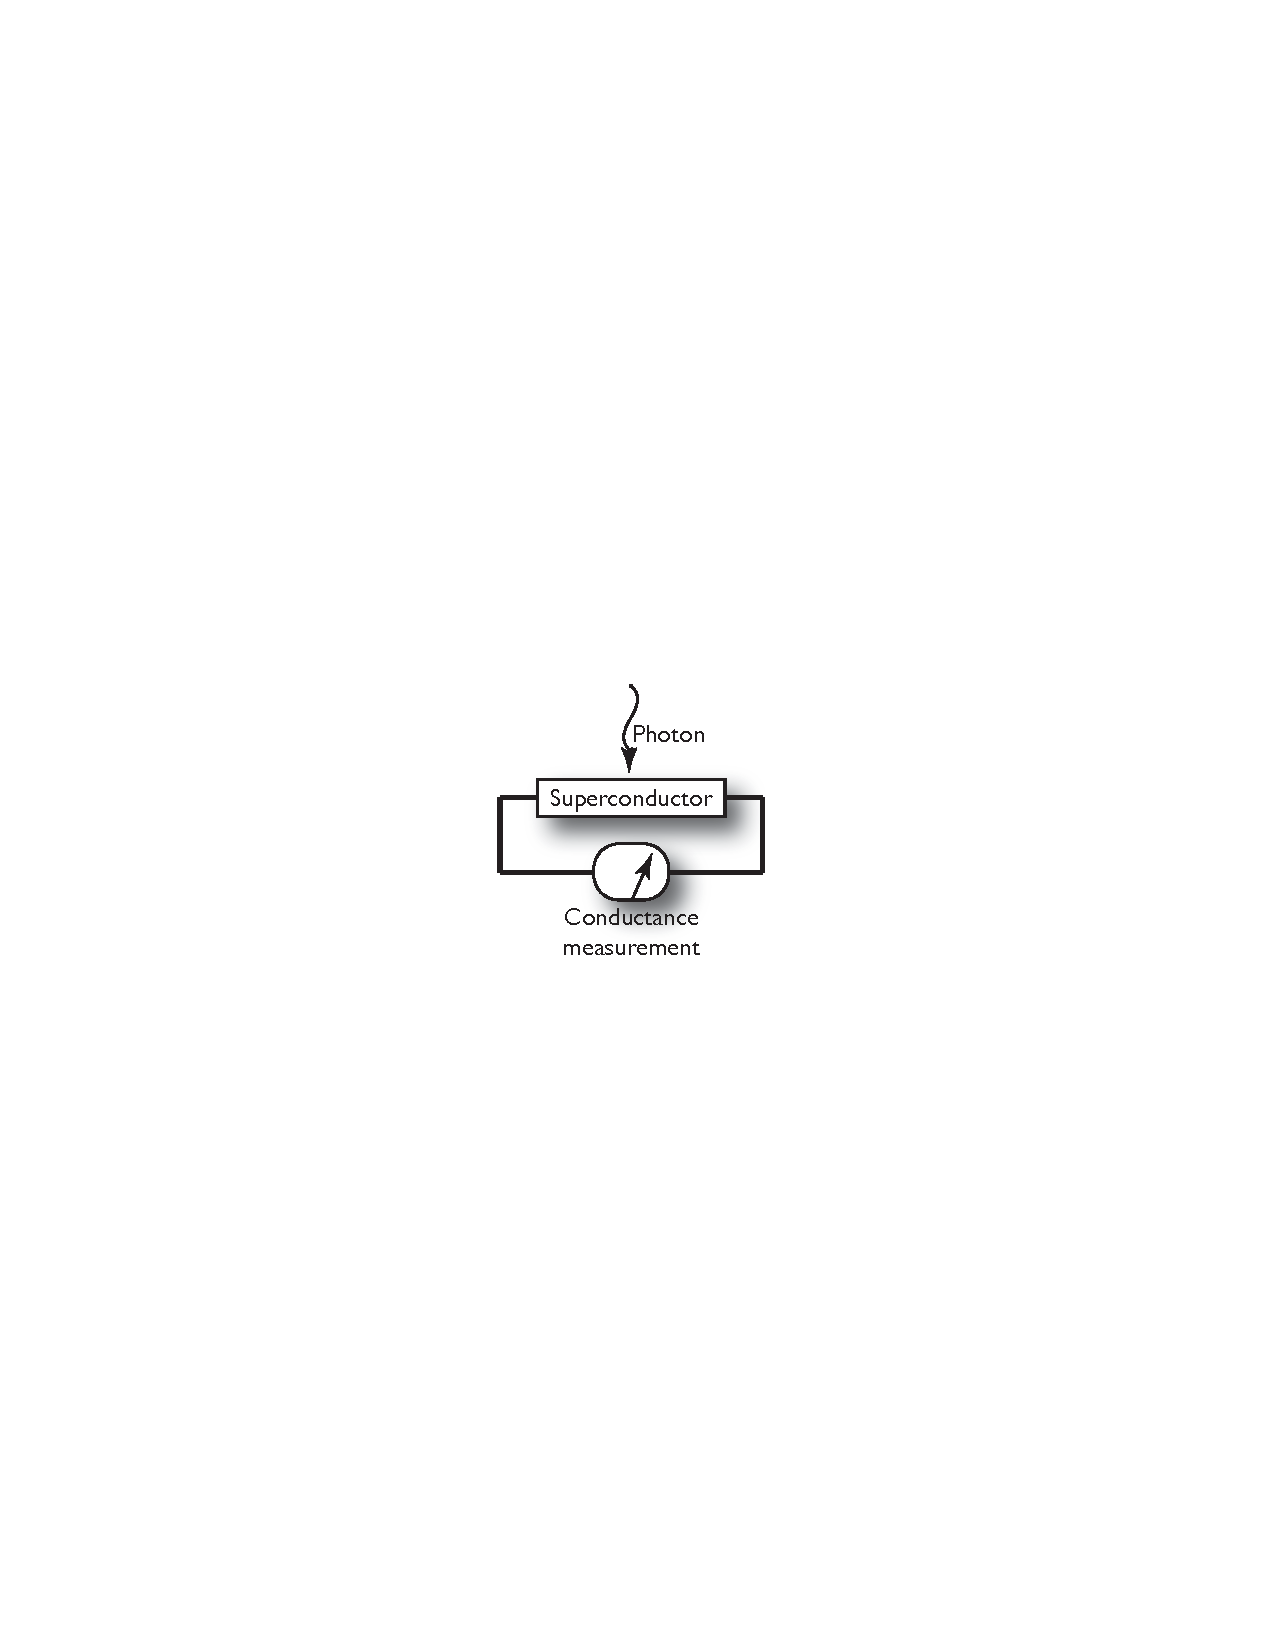
\includegraphics[clip=true, width=0.25\textwidth]{superconducting_detector}
\captionspacefig \caption{A superconducting photo-detector. A superconductor is held at just below its critical temperature. The absorption of a photon is sufficient to heat it above the critical temperature, yielding a detectable change in conductance across the device.} \label{fig:super_det}
\end{figure}

\comment{Is this the same as transition edge sensor (TES)}

%
% Quantum Dot Photo-Detectors
%

\subsubsection{Quantum dot photo-detectors}\index{Quantum dot photo-detectors}

\comment{To do}

%
% Photo-Diodes
%

\subsubsection{Photo-diodes}\index{Photo-diodes}

\comment{To do}

%
% Experimental issues
%

\subsubsection{Experimental issues}

The key parameter of interest in a photo-detector, in addition to whether or not it is number-resolving, is its efficiency\index{Detector efficiency}, $\eta$ -- the probability that a given incident photon will trigger the detector. For most applications, the goal is to maximise $\eta$. As one might expect, there is a direct tradeoff between $\eta$ and cost, with very high-efficiency detectors often economically out of reach for many experimentalists. Also of interest is the `dark-count' rate -- the rate at which the detector falsely clicks in the absence of photons. However, this is often ignored as modern detectors typically exhibit very low dark-count-rates.

Mathematically, the measurement operators for number-resolved detection are,
\begin{align}\index{Number-resolved photo-detectors}
\hat\Pi_n = \eta^{n} \sum_{m=n}^\infty \binom{m}{n} (1-\eta)^{m-n} \ket{m}\bra{m},
\end{align}
for measurement outcome $n$, in the photon-number basis. And for non-number-resolved detection,
\begin{align}\index{Non-number-resolved photo-detectors}
&\hat\Pi_0 = \sum_{m=0}^\infty (1-\eta)^{m} \ket{m}\bra{m}, \nonumber \\
&\hat\Pi_{>0} = \mathbb{\hat{I}} - \hat\Pi_0.
\end{align}
Thus, inefficiency results in projection onto the wrong photon-number, making measurement outcomes incorrect.

In addition to their operation in the photon-number basis, photo-detectors exhibit spatio-temporal characteristics, which affect their operation in quantum information processing protocols \cite{RohdePDReview}. For example, imperfect spectral response can undermine photonic interference, affecting which-path erasure protocols, such as Bell state projection (Sec.~\ref{sec:bell_proj}). However, in many cases this can be improved upon using spectral filtering or time-gating techniques, also at the expense of experimental complexity and resource overhead.

Furthermore, photo-detectors are subject to `dead-time'\index{Dead-time}, which renders them inactive for a finite recovery period following a detection event. This is of especial importance in time-bin-encoded schemes (Sec.~\ref{sec:time_bin}), where detectors must resolve photons over very short timescales on the order of nanoseconds. Dead-time can be modelled as a time-dependent efficiency of the form,
\begin{align}
\eta(t) = \left\{\begin{array}{cc}
 0, & t<\tau_\mathrm{dt} \\
 \eta_\mathrm{ss}, & t\geq\tau_\mathrm{dt} \\
\end{array}\right.,
\end{align}
where $t$ is time, $\tau_\mathrm{dt}$ is the detector's deadtime, and $\eta_\mathrm{ss}$ is the detector's steady-state efficiency (i.e when not dead).

Photo-detectors of all types are inevitably subject to `dark-counts'\index{Dark-counts}, whereby thermal noise\index{Thermal noise}, either within the detector or coupled from the noisy external environment, triggers non-existent detection events. The distribution follows exactly that of the thermal state photon-number distribution (Sec.~\ref{sec:thermal_states}). Thus, the probability of $n$ dark-counts occurring is,
\begin{align} \index{Thermal distribution}
p_\mathrm{dc}(n) = e^{-|\alpha|^2} \frac{|\alpha|^2}{n!},
\end{align}
where $\alpha$ is a parameterisation of the temperature of the environmental noise. Fortunately, modern detector technology is able to keep dark-count rates very low, making this far less of an issue than the aforementioned ones, loss being the dominant.

Finally, all photo-detection techniques are subject to some degree of `time-jitter'\index{Time-jitter} -- noise in the detector's reported time of detection. This can be extremely important in the context of temporal mode-matching, where post-selection upon detection events in an extremely narrow time-window effectively enforces temporal indistinguishability.

%
% Multiplexed Photo-Detection
%

\subsection{Multiplexed photo-detection}\index{Multiplexed photo-detection}

Number-resolved detectors are the more challenging ones to experimentally realise. However, using multiplexing techniques\index{Multiplexed photo-detection}, non-number-resolved detectors can be used to closely approximate number-resolution \cite{bib:Fitch03, bib:Banaszek03, bib:Achilles04, bib:RohdeCompDet07}, at the expense of an (efficient) overhead in the complexity of the experiment, which comes at a cost. 

Specifically, there is a direct tradeoff between the confidence in photon-number outcomes, and experimental overhead. The idea behind this is simple. We spread out an $n$-photon state evenly across a large number of modes, $m$, and detect each one independently using a non-number-resolved photo-detector. If \mbox{$m\gg n$}, it is unlikely that more than a single photon will reach any given detector. Thus, by summing the total number of clicks across all detectors, we closely approximate the true photon-number. This multiplexing can be performed in the spatial- or temporal-domains, shown in Fig.~\ref{fig:det_mult}, and has been a widely employed technique in laboratories without access to expensive number-resolved detectors.

Mathematically, we are interested in the probability \mbox{$P(n_\mathrm{meas}=n_\mathrm{inc})$} that the measured number of photons ($n_\mathrm{meas}$) matches the actual number of incident photons ($n_\mathrm{inc}$). The structure of this expression will vary enormously depending on the details of the architecture (e.g multi-port interferometer vs fibre-loop). However, \cite{rohdeHuntington} presented a very general mathematical formalism applicable to all architectural variants. The simplest case to consider is the multi-port interferometer, owing to its perfect symmetry. The probability is simply the probability that no output mode from the multi-port contain multiple photons. A quick calculation yields,
\begin{align}
	P(n_\mathrm{meas}=n_\mathrm{inc}) = \frac{\eta^n m!}{m^n(m-n)!},
\end{align}
for efficiency $\eta$, not accounting for other lesser errors such as dark-counts. This is shown in Fig.~\ref{fig:multiplexed_pd}. For perfect efficiency, \mbox{$\eta=1$}, this probability always approaches unity in the limit of a large number of modes,
\begin{align}
\lim_{m\to\infty}P(n_\mathrm{meas}=n_\mathrm{inc})=1.
\end{align}

\begin{figure}[!htbp]
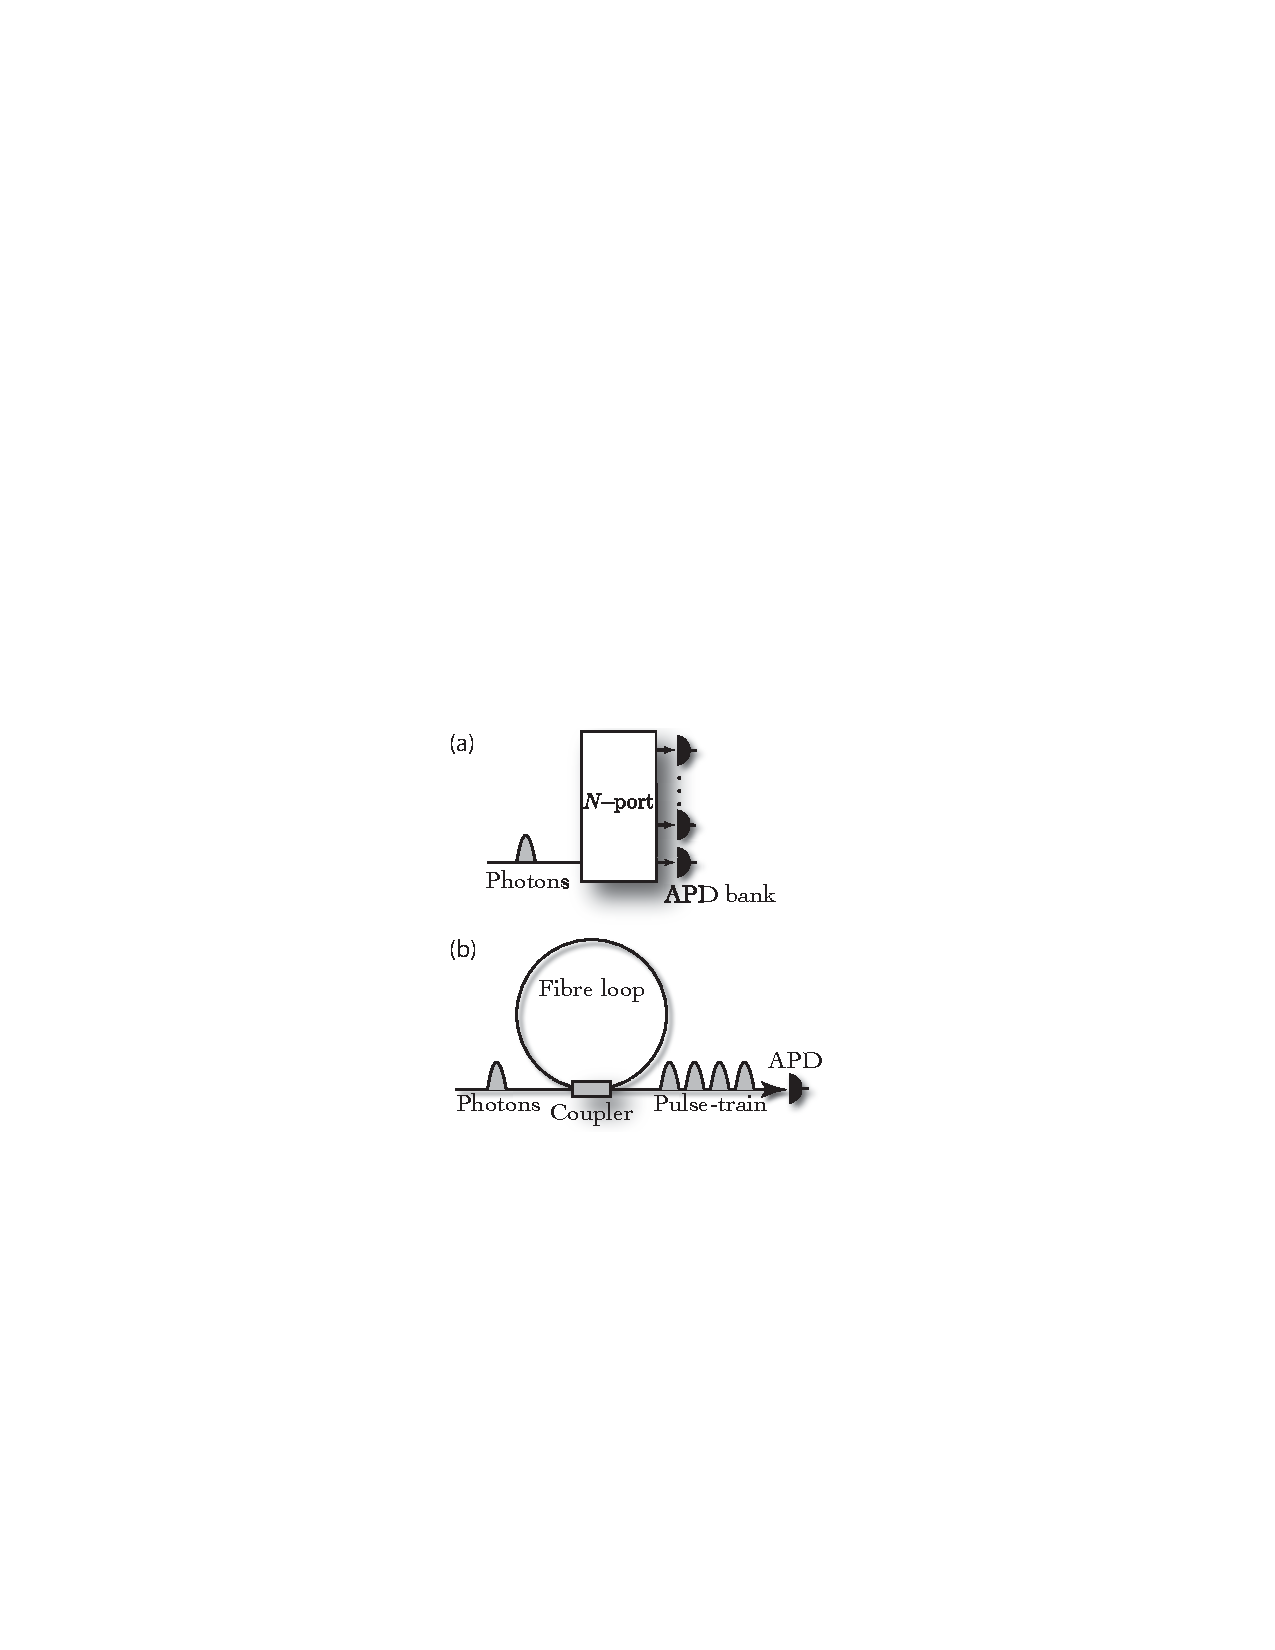
\includegraphics[clip=true, width=0.35\textwidth]{detector_multiplexing}
\captionspacefig \caption{Multiplexed number-resolved photo-detection using non-number-resolved photo-detectors. The principle is to spread out (as uniformly as possible) a multi-photon state across a large number of modes, sufficiently large that it is unlikely that more than one photon will be present in any given mode. Then, the sum of the number of clicks at each mode closely approximates the incident photon-number. (a) In the spatial domain. (b) In the temporal domain. The advantage of employing the temporally multiplexed architecture is that only a single detector is required, unlike the multiple independent detectors required in the spatially multiplexed scheme. However this requires that the dead-time\index{Dead-time} of the detector is less than the round-trip time of the fibre loop. An alternate, but conceptually equivalent approach is to spatially disperse the optical field across a charge-coupled device (CCD)\index{Charge-coupled device (CCD)}, much like that found in a regular digital camera, except with single-photon resolution per-pixel. This achieves an effectively very large number of optical modes.} \label{fig:det_mult}
\end{figure}

\begin{figure}[!htbp]
	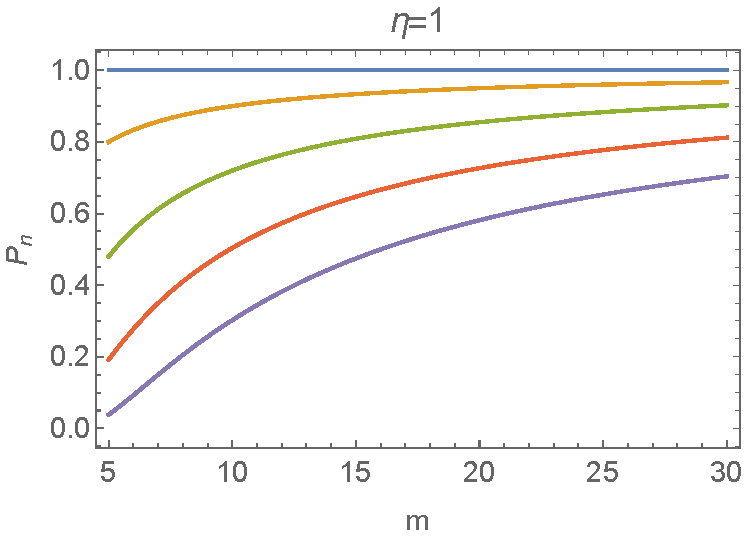
\includegraphics[clip=true, width=0.475\textwidth]{multiplexed_detector}
	\captionspacefig \caption{Probability of a balanced multiplexed detector inferring the correct number of photons with $n$ incident photons across $m$ modes. The detectors have perfect efficiency, \mbox{$\eta=1$}, and all other errors are ignored. The number of incident photons ranges from \mbox{$n=1$} (top) to \mbox{$n=5$} (bottom). All curves asymptotically approach \mbox{$P_n=1$} for large $m$.}\label{fig:multiplexed_pd}
\end{figure}

%
% Homodyning
%

\subsection{Homodyning} \label{sec:homodyne} \index{Homodyne detection}

A homodyne detector interferes a state with a coherent state on a beamsplitter, which acts as a phase-reference\index{Phase-reference}, before photo-detecting both output modes and taking the difference in the photon count-rates (Fig.~\ref{fig:homodyne}).

By sweeping through the amplitude and phase of the reference beam, we are able to directly sample points in phase-space, allowing the Wigner function\index{Wigner function} -- which is isomorphic to the density operator -- of an unknown state to be fully reconstructed.

Equivalently, homodyne detection can directly sample the position ($\hat x$) and momentum ($\hat p$) operators, or arbitrary linear combinations of the two. 

The operation of homodyne measurement is most easily visualised in phase-space, where it can be regarded as integrating along an infinite line with arbitrary rotation determined by the phase-reference.

This measurement technique is typically applied to CV states rather than photon-number states. While conceptually straightforward, preparing the reference beam requires a coherent source, which can become costly (Sec.~\ref{sec:coherent_states}).

\begin{figure}[!htbp]
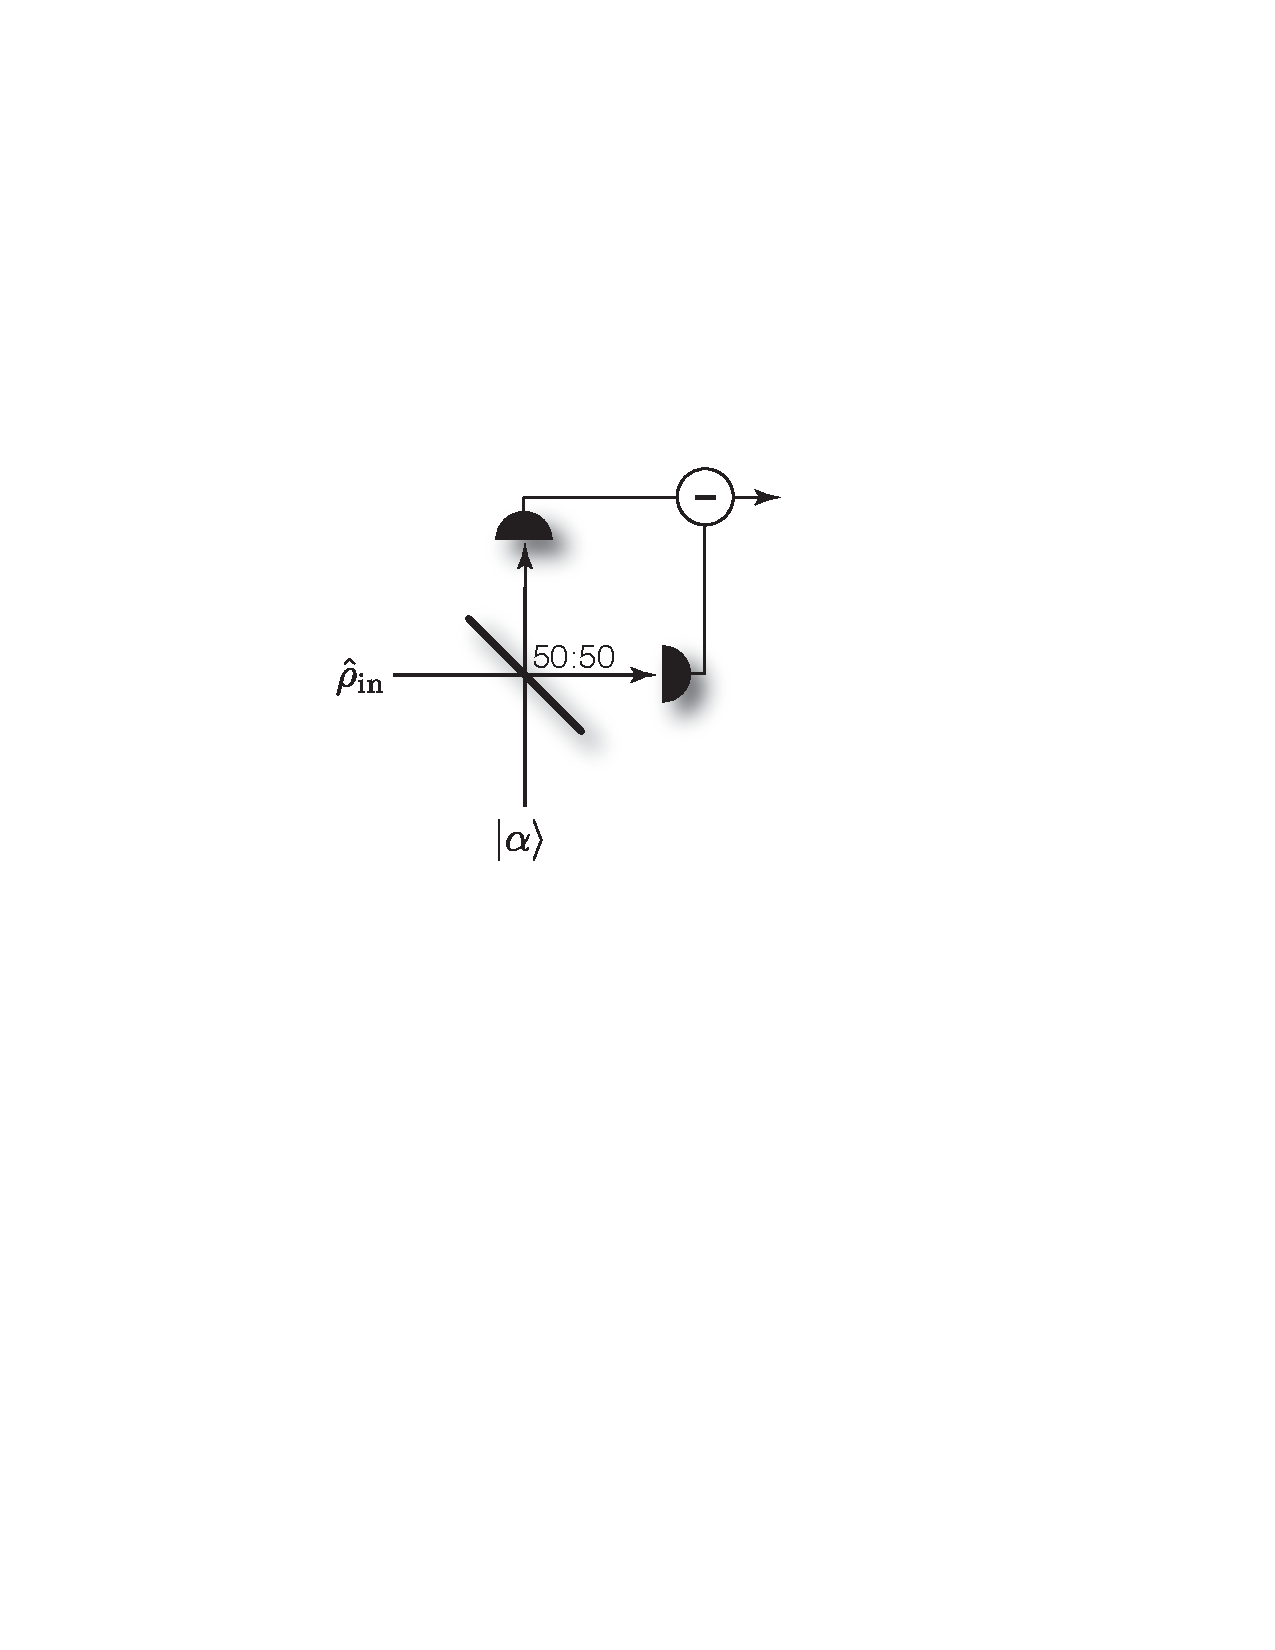
\includegraphics[clip=true, width=0.3\textwidth]{homodyne}
\captionspacefig \caption{Homodyne detection of an unknown optical state $\hat\rho_\mathrm{in}$, by mixing it with a reference coherent state $\ket\alpha$ on a 50:50 beamsplitter, and taking the difference in the photo-detection rates at the output modes. By sweeping through the phase and amplitude of $\ket\alpha$, we can directly sample the Wigner function of $\hat\rho_\mathrm{in}$, allowing its full reconstruction.} \label{fig:homodyne}
\end{figure}

%
% Bell State & Parity Measurements
%

\subsection{Bell state \& parity measurements} \label{sec:bell_proj} \index{Bell measurements}

For the purposes of which-path erasure, essential for optical cluster state (Sec.~\ref{sec:CSQC}) preparation and quantum teleportation (Sec.~\ref{sec:teleport}), Bell state measurements [i.e projections onto the Bell basis given in Eq.~(\ref{eq:bell_basis})], or equivalently parity measurements, are important.

To realise this, there are two primary options. The first is to use a CNOT gate, for example an LOQC gate (Sec.~\ref{sec:KLM_univ}). The second is to perform a \textit{partial} Bell state projection using a polarising beamsplitter (PBS) -- a beamsplitter which completely transmits vertical polarisation, and completely reflects horizontal polarisation \cite{bib:BraunsteinMann95}.

In the Heisenberg picture, the transformation of the photonic creation operators implemented by a PBS is,
\begin{align}\index{Polarising beamsplitters}
\hat{h}_1^\dag &\to \hat{h}_2^\dag, \nonumber \\
\hat{h}_2^\dag &\to \hat{h}_1^\dag, \nonumber \\
\hat{v}_1^\dag &\to \hat{v}_1^\dag, \nonumber \\
\hat{v}_2^\dag &\to \hat{v}_2^\dag,
\end{align}
where $\hat{h}_i^\dag$ ($\hat{v}_i^\dag$) are the horizontal (vertical) creation operators for the $i$th mode. The measurement projectors implemented by the PBS, when both modes are measured in the diagonal ($+/-$) basis\footnote{By measuring in the diagonal basis we erase information about whether photons were horizontally or vertically polarised, thereby projecting onto the coherent subspace of both possibilities. Such a diagonal basis measurement may be implemented using a wave-plate to perform a Hadamard polarisation rotation, followed by another PBS, separating the horizontal and vertical components, which are then independently measured via regular photo-detection.}, are then,
\begin{align}
	\hat\Pi_\mathrm{Bell}^+ &= \ket{H,H}\bra{H,H}+\ket{V,V}\bra{V,V}, \nonumber \\
	\hat\Pi_\mathrm{Bell}^- &= \ket{H,H}\bra{H,H}-\ket{V,V}\bra{V,V}, \nonumber \\
	\hat\Pi_
	\mathrm{HV} &= \ket{H,V}\bra{H,V}, \nonumber \\
\hat\Pi_
	\mathrm{VH} &= \ket{V,H}\bra{V,H},
\end{align}
where the former two represent successful projection onto the Bell basis, and the latter two represent failures, effectively measuring both modes in the $H/V$ basis. This approach is described in Fig.~\ref{fig:partial_bell}.

Technically, $\hat\Pi^\pm_\mathrm{Bell}$ are not Bell measurements, but rather projections onto the even parity subspace. A true Bell projection would implement $\ket{\Phi^\pm}\bra{\Phi^\pm}$. However, in an optical context the two terms are often used interchangeably, since they exhibit effectively the same behaviour, given that the detection process is destructive.

Bell projections using CNOT gates can be implemented with arbitrarily high success probability in principle. However, in most scenarios of interest (such as cluster state preparation and entanglement purification) Bell projection using a PBS succeeds with probability of $1/2$, since a PBS is only able to uniquely distinguish two of the four Bell states. To its advantage, such `partial' Bell measurements only require high HOM visibility, avoiding the need for the interferometric stability inherent internally within LOQC CNOT gates.

\begin{figure}[!htbp]
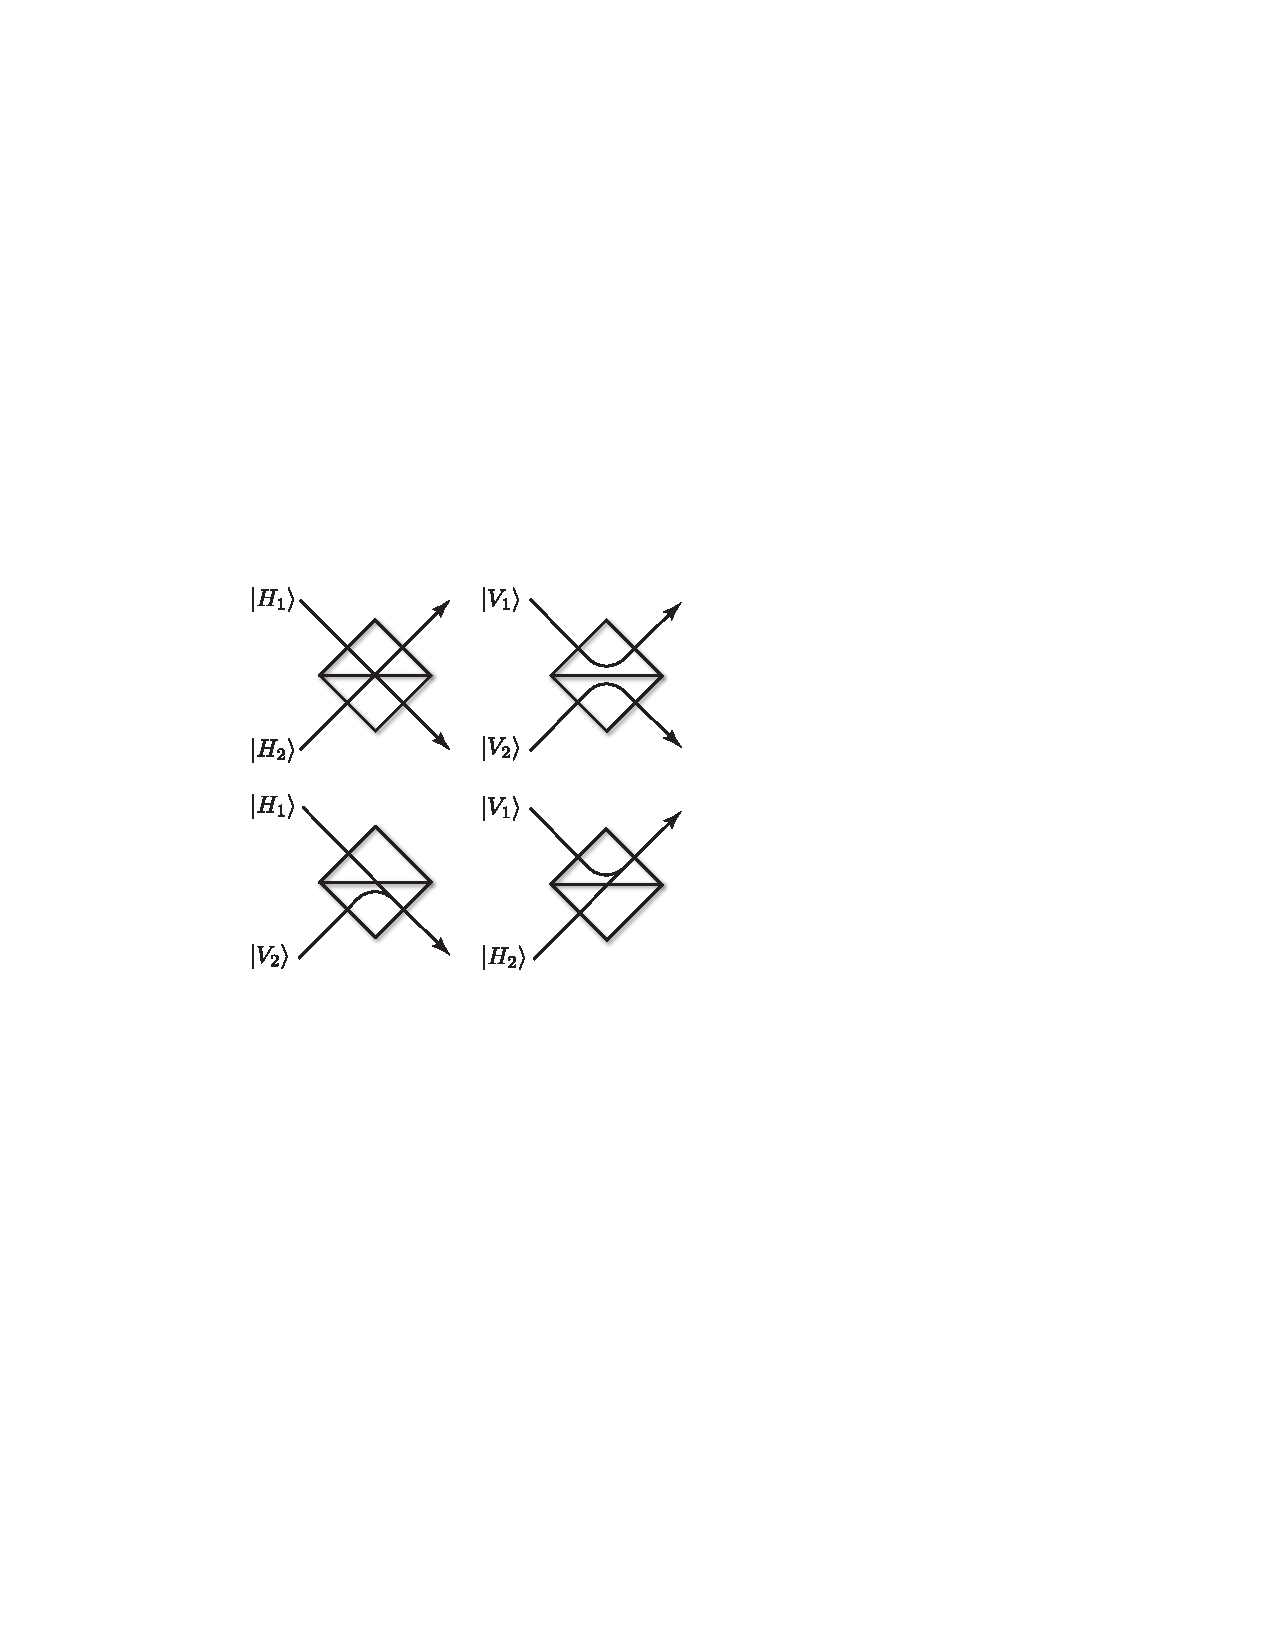
\includegraphics[clip=true, width=0.375\textwidth]{partial_bell}
\captionspacefig \caption{Partial Bell state projection using a polarising beamsplitter (PBS). The PBS completely transmits horizontally polarised light, whilst completely reflecting vertically polarised light. Shown are the four possible two-photon input states, and the respective trajectories followed by the photons. To complete the partial Bell projection we measure the output modes in the diagonal basis, \mbox{$\ket{\pm} = \frac{1}{\sqrt{2}}(\ket{H}\pm\ket{V})$}, such that horizontally and vertically polarised photons cannot be distinguished. If the input state was $\ket{H,H}$ or $\ket{V,V}$, we would measure one photon in each output mode (both transmitted or both reflected). Since the detectors cannot distinguish $\ket{H}$ from $\ket{V}$, this effectively projects us onto the coherent superposition of both possibilities (`which-path erasure'), implementing the measurement projector \mbox{$\hat\Pi_\mathrm{Bell}^\pm = \ket{H,H}\bra{H,H}\pm\ket{V,V}\bra{V,V}$}. If, on the other hand, we measure two photons at one output mode, we know with certainty what the polarisations of both incident photons were and we probabilistically implement one of the projectors \mbox{$\hat\Pi_
\mathrm{HV}=\ket{H,V}\bra{H,V}$} or \mbox{$\hat\Pi_
\mathrm{VH}=\ket{V,H}\bra{V,H}$}, effectively performing polarisation-resolved detection upon both modes, which equates to a $\hat{Z}$ measurement on the logical qubits. The practical outcome of this is that, when using a PBS to prepare cluster states, with probability $1/2$ we are able to successfully fuse two smaller cluster states together into a larger one, and with probability $1/2$ we fail to do so, instead removing two qubits from the clusters.} \label{fig:partial_bell}
\end{figure}

While partial Bell state projection using a PBS is relatively straightforward, LOQC CNOT gates (which are very desirable owing to their near-determinism) are very technologically challenging, with drastic resource overheads, particularly for high success probability. Thus, outsourcing them to the cloud may be very economically efficient.

\comment{Talk about CV equivalent}

%
% Matter Qubits
%

\subsection{Matter qubits} \index{Matter qubits}

Many non-optical systems can be indirectly measured by first entangling optical states with the matter qubits and then measuring the optical state. Because of the entanglement, projective measurement on the optical state teleports the measurement onto the matter qubit.

In Fig.~\ref{fig:barrett_kok} we illustrate a scheme for entangling two $\lambda$-configuration atoms using which-path erasure. Consider just one of these qubits in isolation. If a $\pi$-pulse is applied to the atom, the $\ket{\!\downarrow}$ state is excited to the $\ket{e}$ state, after which, upon relaxation, it emits a photon. Thus, upon measurement, the presence or absence of a photon directly indicates whether the qubit was in the $\ket{\!\uparrow}$ or $\ket{\!\downarrow}$ state.

The attractive feature of this is that although the matter qubit is stationary, its indirect measurement via optical coupling may be performed over arbitrary distances across the optical network, allowing the measurement stage to be outsourced. This includes entangling measurements, useful for, for example, cluster state preparation (Sec.~\ref{sec:CSQC}).

%
% Quantum non-demolition measurement
%

\subsection{Quantum non-demolition measurement}\index{Quantum non-demolition measurement (QND)}

\comment{To do! List abbrev.}

%
% Weak Measurement
%

\subsection{Weak measurement}

\comment{To do}

%
% Evolution
%

\section{Evolution}

\dropcap{T}{he} evolution of optical states represents an extremely broad category of quantum operations, including: passive linear optics; post-selected linear optics; non-linear optics; and, light-matter interactions. Clearly, the items in this list present technological challenges, inaccessible to many users.

The error models in the evolution of optical states are largely accounted for by those discussed in Sec.~\ref{sec:errors_in_nets}. 

%
% Linear Optics
%

\subsection{Linear optics} \label{sec:LO_ev_archs} \index{Linear optics evolution}

Linear optics networks \cite{bib:TanRohdeRev} implement unitary linear maps on the photonic creation operators, of the form,
\begin{align} \label{eq:LO_unitary_map}
\hat{U}\hat{a}_i^\dag \hat{U}^\dag \to \sum_{j=1}^m U_{i,j} \hat{a}^\dag_j,
\end{align}
where $\hat{a}^\dag_i$ is the photonic creation operator on the $i$th of the $m$ modes, and $U$ may be any $\mathrm{SU}(m)$ matrix. It was shown by \cite{bib:Reck94} that arbitrary transformations of this form may be decomposed into $O(m^2)$ linear optical elements (beamsplitters and phase-shifters), enabling efficient construction of arbitrary linear transformations.\index{Linear optics decompositions} Furthermore, the algorithm for determining the decomposition of such transformations has polynomial classical runtime (i.e residing in \textbf{P}\index{P}). Note that the original Reck \textit{et al.} decomposition is not unique, and various other topologies of optical elements also enable universality \cite{???}.

Each individual beamsplitter in such a decomposition is an arbitrary $\mathrm{SU}(2)$ matrix acting on two photonic creation operators, $\hat{a}^\dag$ and $\hat{b}^\dag$,
\begin{align}\index{Beamsplitters}
\begin{pmatrix}
\hat{a}^\dag_\mathrm{out} \\
\hat{b}^\dag_\mathrm{out}
\end{pmatrix}=\begin{pmatrix}
U_{11} & U_{12} \\
U_{21} & U_{22}
\end{pmatrix}\begin{pmatrix}
\hat{a}^\dag_\mathrm{in} \\
\hat{b}^\dag_\mathrm{in}
\end{pmatrix}.
\end{align}
When operating in the polarisation basis, wave-plates\index{Wave-plates} enable the same transformation as beamsplitters do in dual-rail encoding. The phase-shifters implement the unitary operation,\index{Phase-shifters}
\begin{align}
\hat\Phi(\phi)=e^{-i\phi\hat{n}},
\end{align}
or equivalently in the Heisenberg picture,
\begin{align}
\hat{U}\hat{a}^\dag\hat{U}^\dag \to e^{-i\phi}\hat{a}^\dag,
\end{align}
for phase-shift $\phi$.

These linear optics evolutions are most commonly implemented using either:
\begin{itemize}
\item Bulk optics: discrete optical elements are arranged on an optical table.\index{Bulk optics}
\item Time-bin architectures: time-bin encoded qubits (Sec.~\ref{sec:time_bin}) evolve through delay lines and interfere at a single central optical component.\index{Time-bin encoding}\index{Fibre-loops}
\item Integrated waveguides: all passive components are etched into a chip.\index{Waveguides}
\end{itemize}
These three main contenders are illustrated in Fig.~\ref{fig:LO_archs}.

\if 2\pubmode
	\begin{figure}[!htbp]
	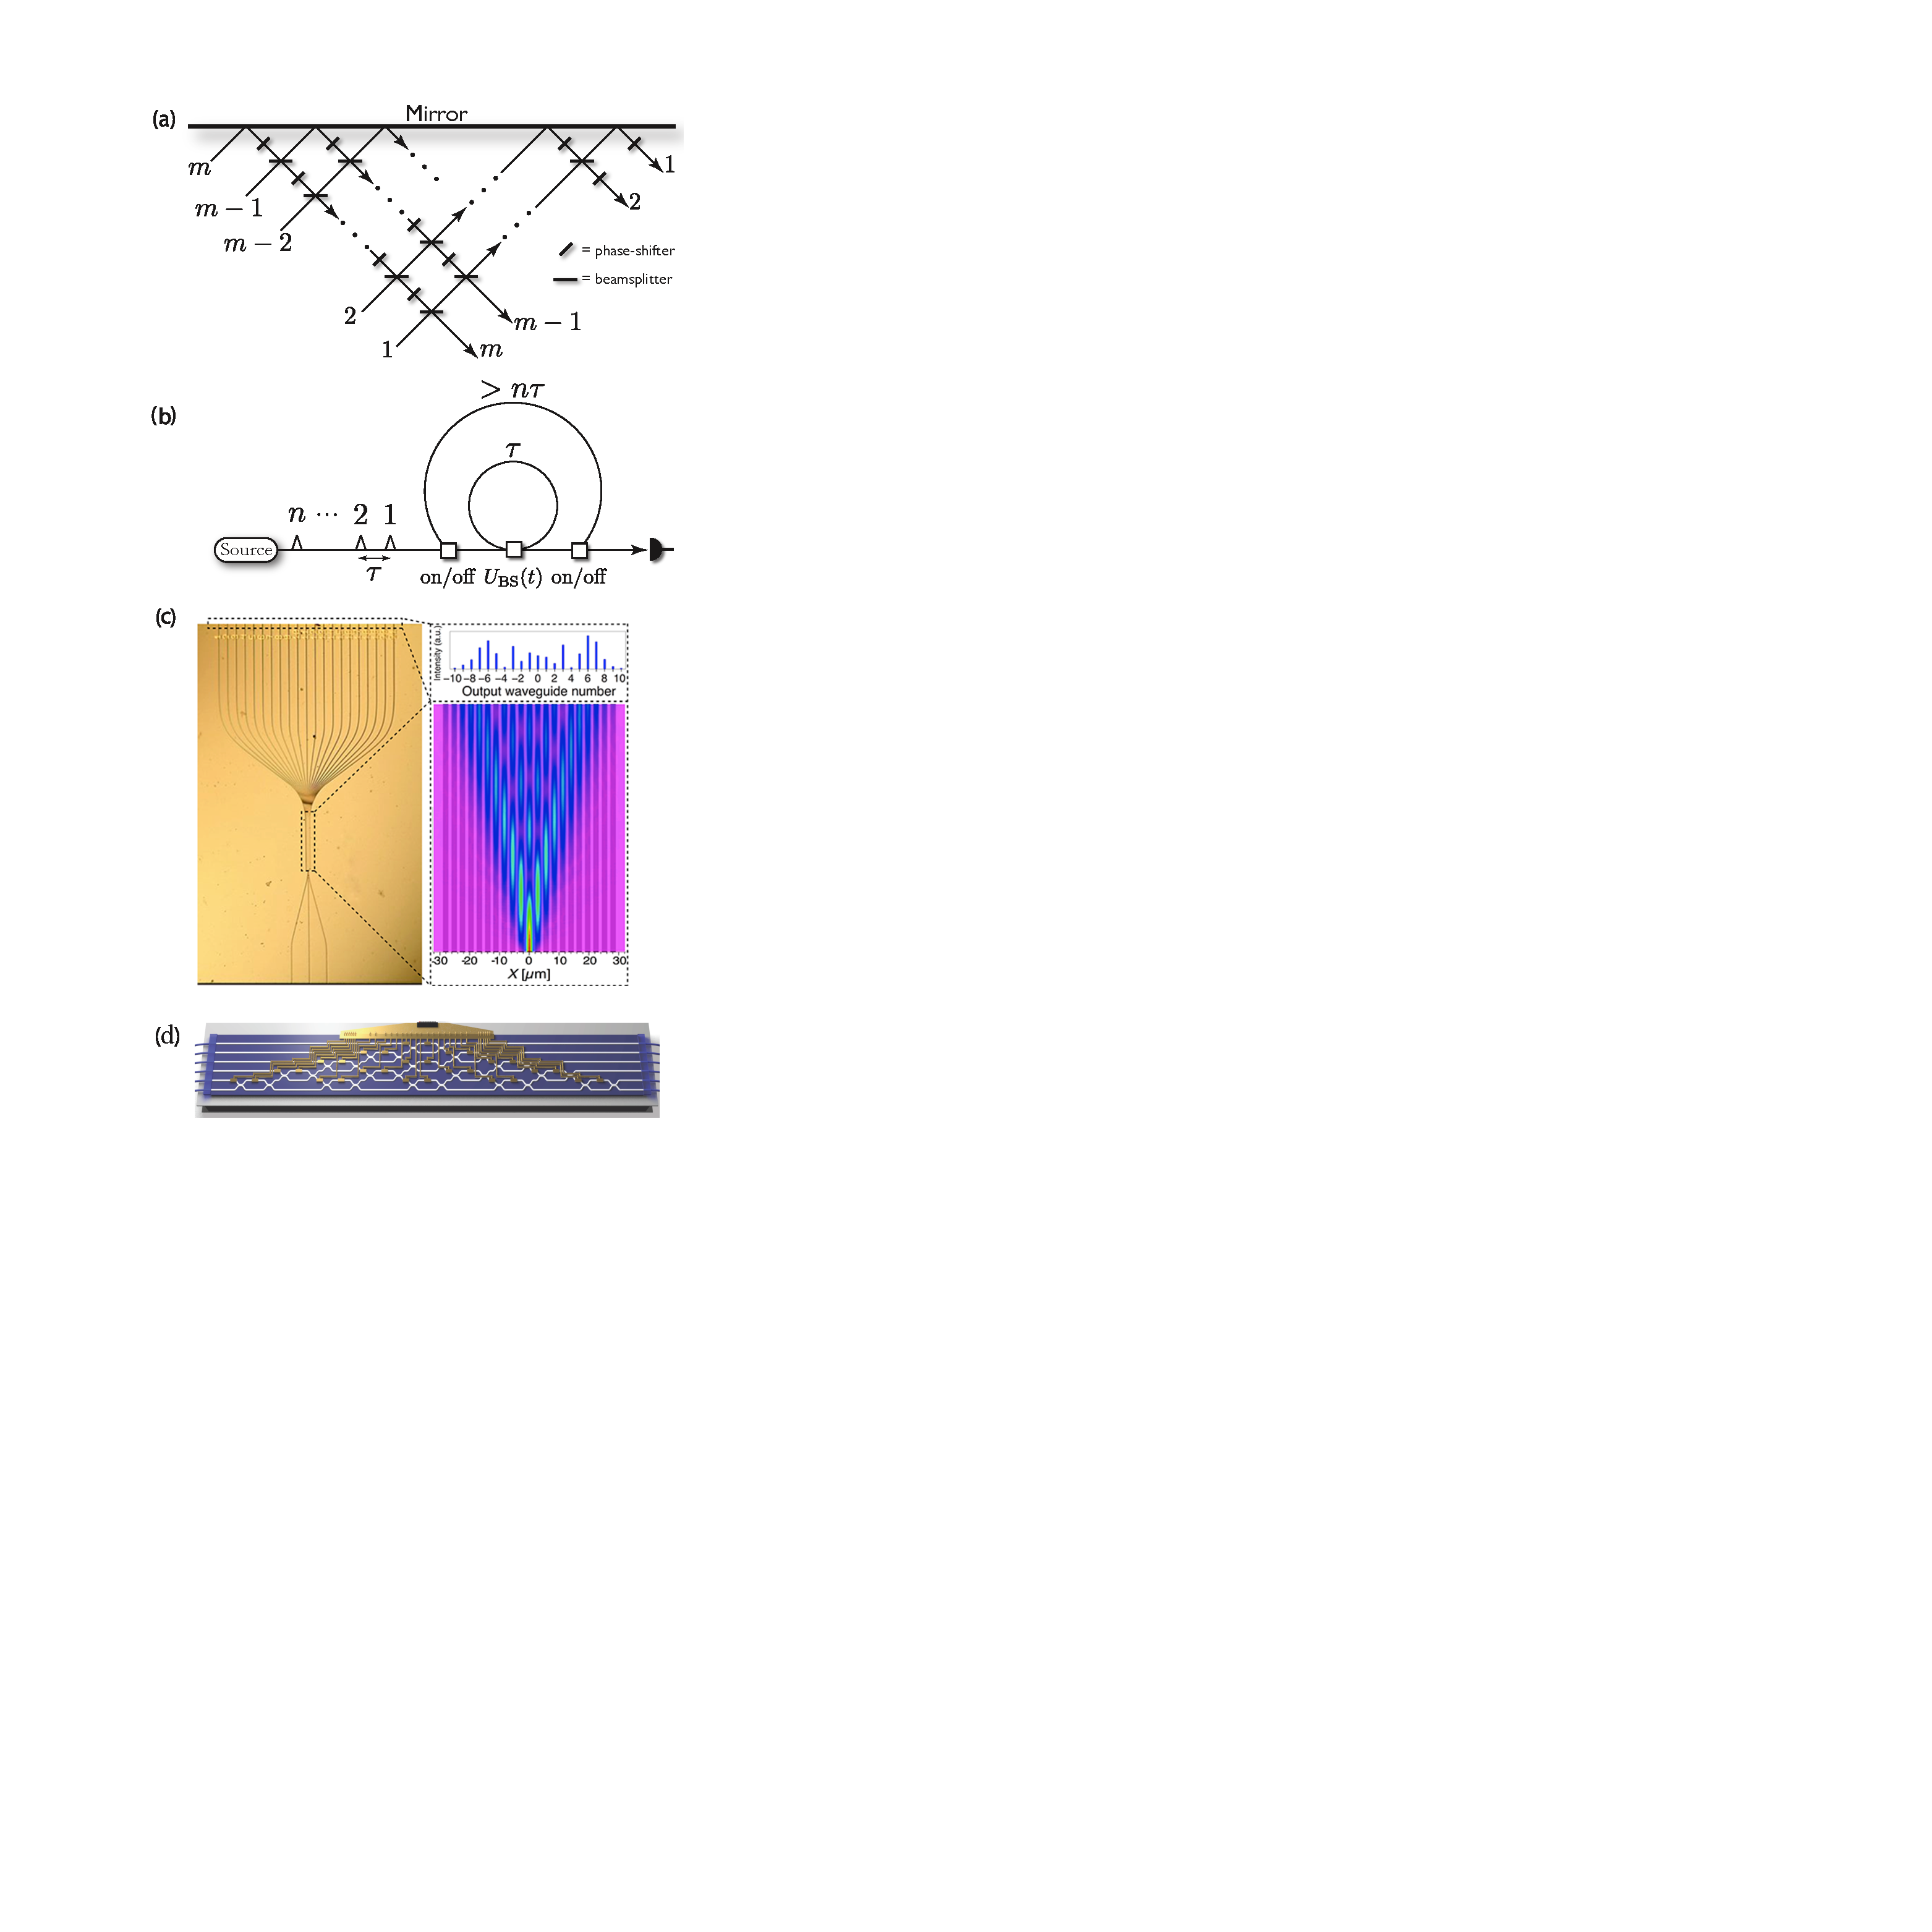
\includegraphics[clip=true, width=0.475\textwidth]{LO_archs_long}
	\captionspacefig \caption{The three primary approaches for implementing linear optics transformations. (a) Bulk optics\index{Bulk optics}, where each optical mode is spatially encoded, and the linear transformation is decomposed into a discrete array of beamsplitters and phase-shifters, an appropriate choice of which enables arbitrary linear optics transformations to be implemented. (b) Time-bin encoding\index{Time-bin encoding}\index{Fibre-loops}, where each optical mode is designated a distinct time-bin. Fibre-loops meeting at dynamically reconfigurable beamsplitters enable arbitrary linear transformations to be implemented. (c) Integrated wave-guide chips\index{Waveguides}, where evanescent coupling between neighbouring wave-guides within a chip facilitates interference between modes (graphic courtesy of Alberto Peruzzo \cite{bib:PeruzzoQW}). (d) Integrated wave-guide chip with electrically controllable phase-shifters, implementing a programmable, universal \mbox{$6\times 6$} linear optics network (graphic courtesy of Jeremy O'Brien \cite{bib:UniversalLOOBrien}\comment{Get permission}).} \label{fig:LO_archs}
	\end{figure}
\else
	\begin{figure*}[!htbp]
	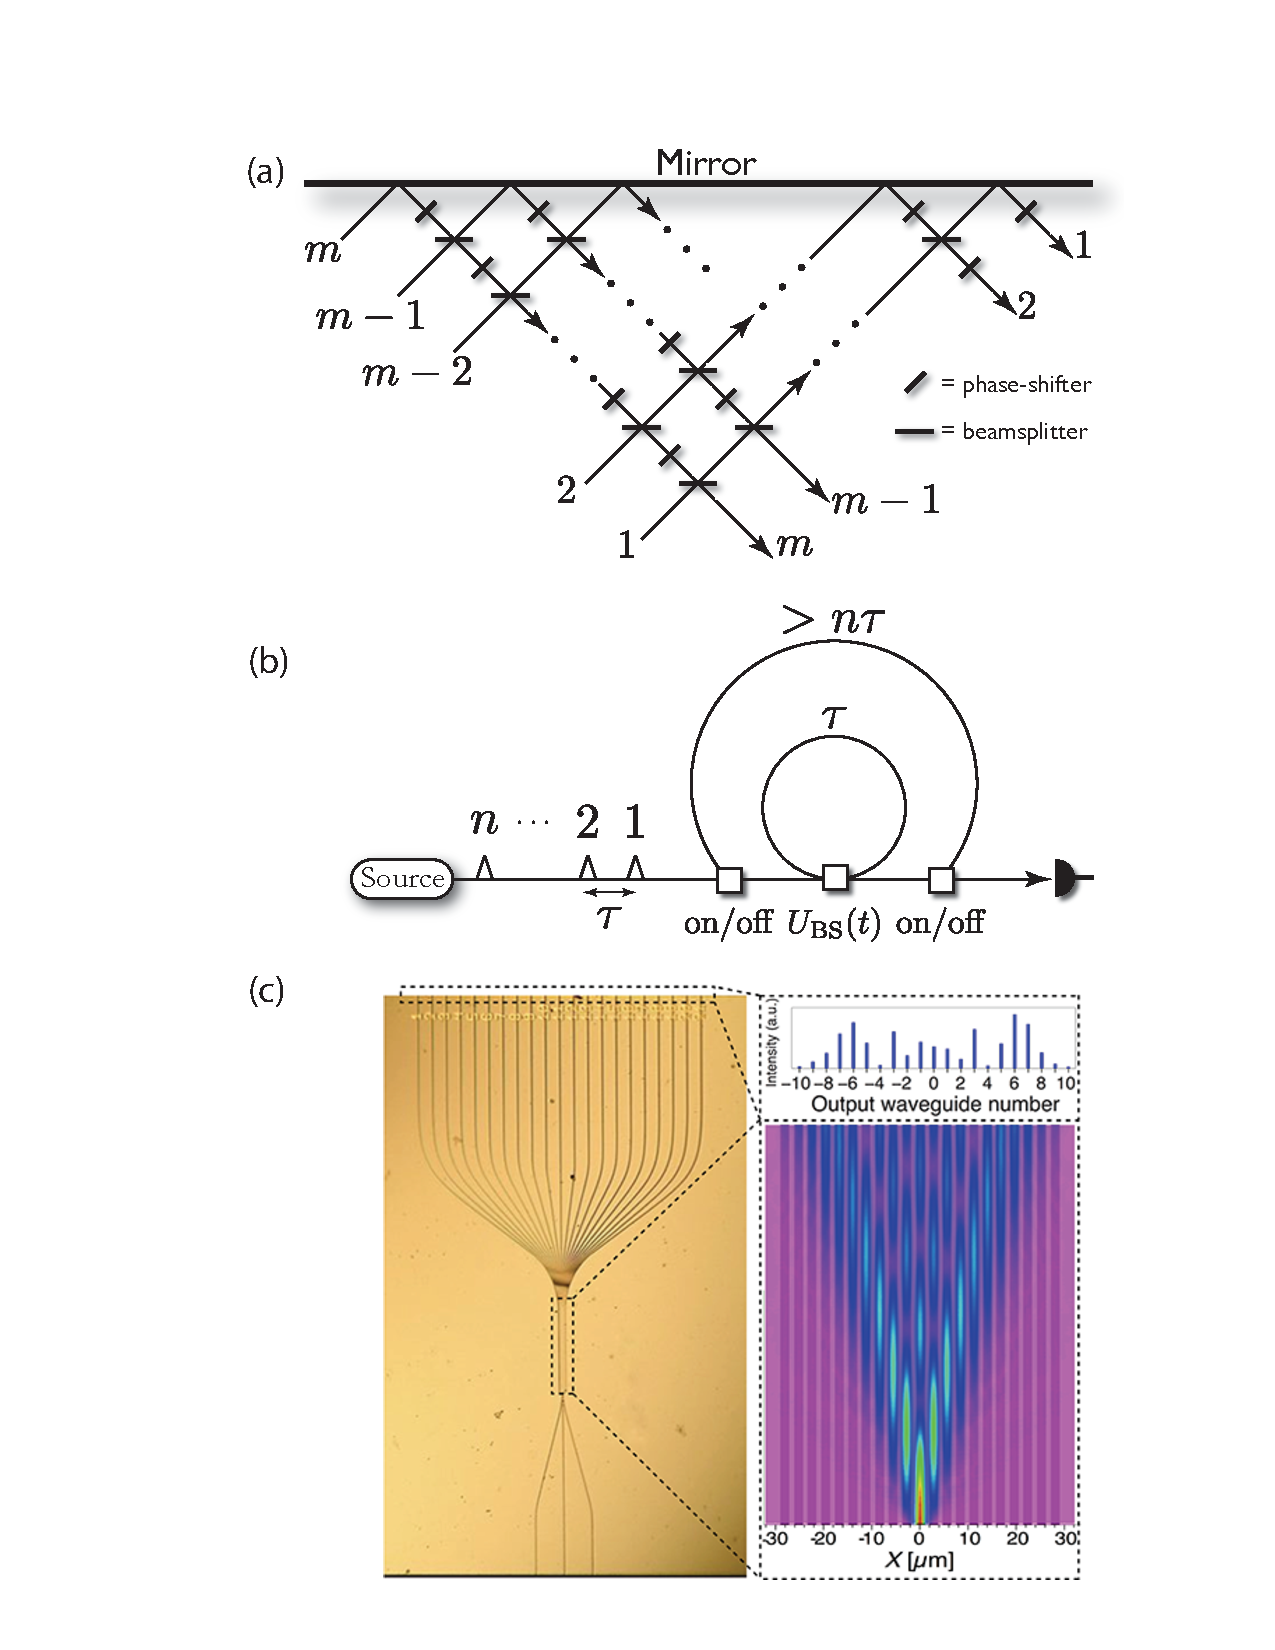
\includegraphics[clip=true, width=\textwidth]{LO_archs}
	\captionspacefig \caption{The three primary approaches for implementing linear optics transformations. (a) Bulk optics\index{Bulk optics}, where each optical mode is spatially encoded, and the linear transformation is decomposed into a discrete array of beamsplitters and phase-shifters, an appropriate choice of which enables arbitrary linear optics transformations to be implemented. (b) Time-bin encoding\index{Time-bin encoding}\index{Fibre-loops}, where each optical mode is designated a distinct time-bin. Fibre-loops meeting at dynamically reconfigurable beamsplitters enable arbitrary linear transformations to be implemented. (c) Integrated wave-guide chips\index{Waveguides}, where evanescent coupling between neighbouring wave-guides within a chip facilitates interference between modes (graphic courtesy of Alberto Peruzzo \cite{bib:PeruzzoQW}). (d) Integrated wave-guide chip with electrically controllable phase-shifters, implementing a programmable, universal \mbox{$6\times 6$} linear optics network (graphic courtesy of Jeremy O'Brien \cite{bib:UniversalLOOBrien}\comment{Get permission}).} \label{fig:LO_archs}
	\end{figure*}
\fi

%
% Non-Linear Optics
%

\subsection{Non-linear optics} \label{sec:non_lin_opt} \index{Non-linear optics}

Aside from the linear transformations described above, which are passive and photon-number-preserving, various active, non-linear interactions are also of interest to optical quantum information processing. The most prominent of these are primarily considered as transformations in phase-space (Sec.~\ref{sec:exotic}), using, for example, the Wigner function representation.

The most well-known non-linear transformation is the displacement operation, which translates the Wigner function by some arbitrary amplitude in phase-space, whilst preserving all other features of the phase-space representation. This is described by the unitary operator,\index{Displacement operator}
\begin{align}
\hat{D}(\alpha) = \exp \left[\alpha\hat{a}^\dag - \alpha^*\hat{a}\right],
\end{align}
where $\alpha$ is the displacement amplitude. This transformation is easily implemented by mixing a state on a low-reflectivity beamsplitter with a coherent state of some arbitrary complex amplitude, which determines the displacement amplitude. In the special case of a displacement operator acting on the vacuum state, we obtain a coherent state of equal amplitude, \mbox{$\hat{D}(\alpha)\ket{0}=\ket\alpha$}.

Another common non-linear transformation is squeezing, discussed in Sec.~\ref{sec:squeezed}. This implements the unitary operator\index{Squeezing operator},
\begin{align}
\hat{S}(\xi) = \exp \left[ \frac{1}{2}(\xi^*\hat{a}^2 - \xi{\hat{a}^{\dag 2}})\right],
\end{align}
where $\xi$ is the squeezing parameter, which has the effect of applying a dilation of some arbitrary factor in phase-space.

Thus, jointly, the displacement and squeezing operators enable arbitrary translations and dilations in phase-space. These operations form the basis for CV quantum computing schemes, to be discussed in more detail in Sec.~\ref{sec:CV_QC}.

%
% Non-Optical Systems
%

\subsection{Non-optical systems}

There are countless non-optical systems applicable to quantum information processing applications. For example, quantum computing schemes have been described using: two-level\index{Two-level atoms} or $\lambda$-configuration atoms\index{$\lambda$-configuration systems}; superconducting rings\index{Superconducting rings}; ion traps\index{Ion traps}; atomic ensembles\index{Atomic ensembles}; and countless more.

\comment{Some citations}

From a networking perspective, we are not terribly interested in the inner workings of all these schemes, as we are reasonably confident that optics will be mediating networking, even if other aspects of the protocol are non-optical. Thus, we will not go into great detail about the evolution of non-optical systems. Instead, for our purposes, the relevant issue is interfacing between optical and non-optical systems, such that networking protocols between them may be implemented. Optical interfacing is discussed in detail in Sec.~\ref{sec:opt_inter}.

%
% Quantum Memory
%

\section{Quantum memory} \label{sec:memory} \index{Quantum memory}

\comment{Discuss atomic ensembles, two-level systems, lambda systems, 3-level systems with two ground states (better since no decay).}

\dropcap{A}{} final building block, that will be essential in many networks, is quantum memory, which simply delays a packet by some fixed amount of time, ideally implementing an identity channel ($\hat{\mathbb{I}}$) in the non-temporal degrees of freedom. This will be required when, for example, quantum data packets reach a network bottleneck, and face one of two options: wait, or be discarded. As discussed earlier, discarding quantum packets is often a highly undesirable enterprise, as they often cannot be easily recreated, most notably when entangled with other systems. Quantum memory is an essential component in quantum repeater networks, to be discussed in Sec.~\ref{sec:rep_net}.

%
% Network Graph Representation
%

\subsection{Network graph representation}\index{Network graphs}

Quantum memory is modelled in our network graph representation as per Fig.~\ref{fig:memory}, via a self-loop implementing a process that delays packets. Ideally, the associated process should implement the identity operation in all degrees of freedom, except the temporal one, affecting only the \textsc{Lifetime} metric of the packets passing through it, incrementing it by the duration of the quantum memory.

Note that this is not directly compatible with conventional shortest-path algorithms, which ignore self-loops. One approach is to modify our strategy optimisation algorithms to accommodate self-loops. Alternately, we could construct a `virtual' graph, obtained by adding additional nodes to the network, with connections determined by `unravelling' the self-loops. For example, in Fig.~\ref{fig:memory}, we could eliminate the self-loop, and instead replace $B$ with multiple redundant nodes in series between $A$ and $C$, each associated with their own latency cost.

\begin{figure}[!htbp]
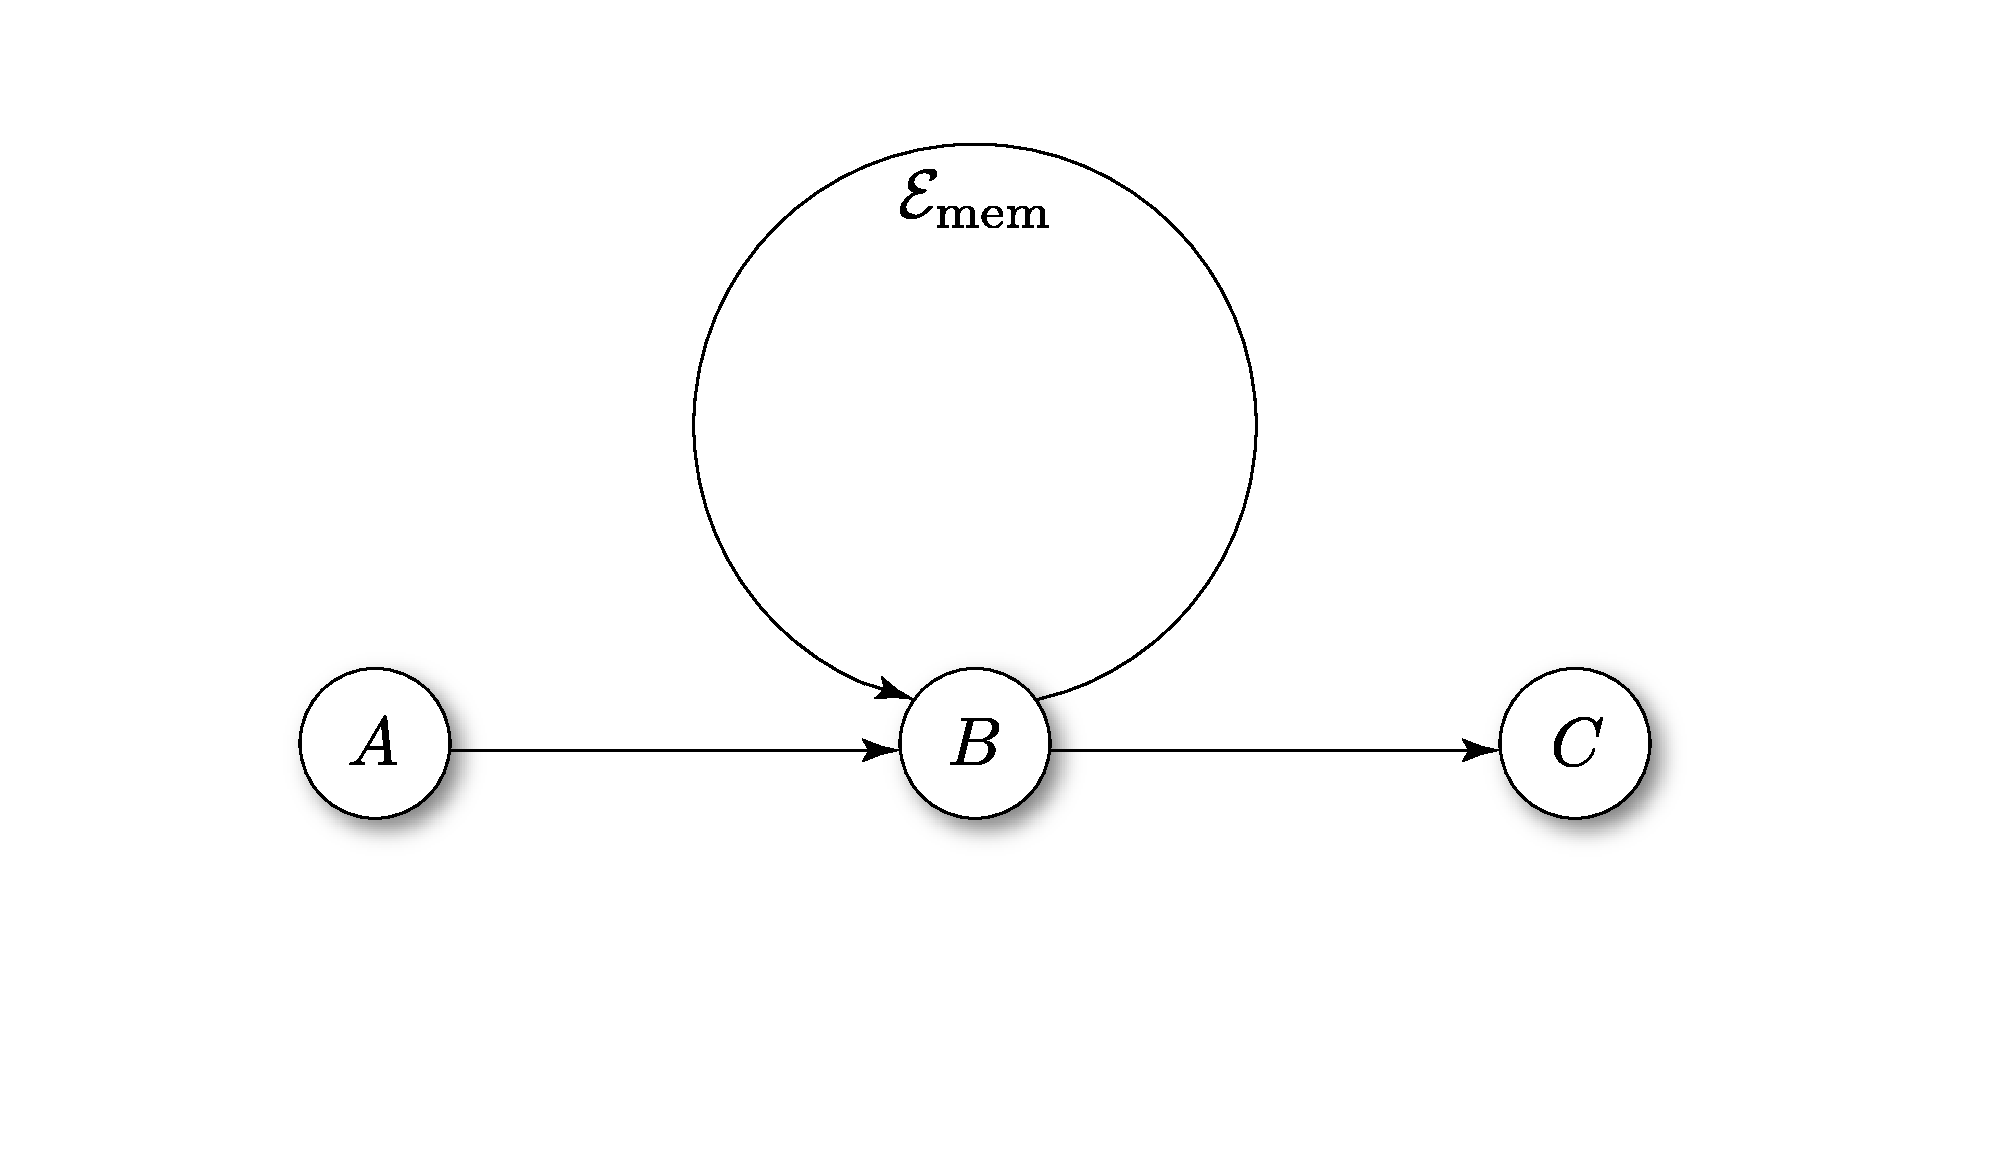
\includegraphics[clip=true, width=0.375\textwidth]{memory}
\captionspacefig \caption{Simple model for a quantum memory via a self-loop that passes through a memory process, $\mathcal{E}_\mathrm{mem}$. Ideally, $\mathcal{E}_\mathrm{mem}$ does not affect any of the costs or attributes of states passing through the link, except for the \textsc{Latency} cost, which is incremented according to the duration of the memory.} \label{fig:memory}
\end{figure}

%
% Physical Implementation
%

\subsection{Physical implementation}

At the physical level, there are two main approaches we could use to put optical states into memory. The first is simply to employ delay lines, either in free-space or in fibre. The second is to interface the state with a non-optical system with a long lifetime, which holds the information content until needed and out-coupled. This can be achieved using, for example, the light-matter interfacing techniques discussed in Sec.~\ref{sec:opt_inter}.

The former is experimentally straightforward, but plagued by loss, and is only suitable over short timescales, on the order of nanoseconds. The latter is more experimentally challenging, but can achieve longer storage times, limited by the lifetime ($T_1$- and $T_2$-times)\index{T$_2$-time}\index{T$_1$-time} of the non-optical system. For some physical systems, this can be very high, on the order of milliseconds for atomic ensemble qubits \cite{bib:Duan01, bib:Duan02, bib:LauratKimble07}, for example, which is typically adequate for the purposes of waiting out network bottlenecks.

%
% Error correction
%

\subsection{Error correction}\index{Quantum error correction (QEC)}

Since quantum memories are subject to errors that accumulate with time, long-life quantum memories will necessarily require error correction mechanisms to preserve qubit states held within them.

To achieve this, standard QEC codes (Sec.~\ref{sec:QOS}) can be employed to encode a number of logical qubits into a larger number of physical qubits, which are held in quantum memory and undergo active error correction. Any of the previously discussed QEC techniques are applicable to this.

An alternate approach is to use W-state encoding\index{W-state encoding} to implement unitary error averaging (Sec.~\ref{sec:error_averaging})\index{Unitary error averaging}, where the unitaries are single-qubit channels \cite{errorfilteringpaper, bib:MadhavPeterLund}. The protocol is shown in Fig.~\ref{fig:W_state_memory}. We begin by using a QFT fanout\index{Fanout} operation to encode a dual-rail encoded qubit\index{Dual-rail encoding} across $N$ optical modes. Each optical mode then feeds into a solid-state qubit (e.g a two-level atom), which ideally implement an identity channel but are inevitably subject to usual error processes such as dephasing and amplitude damping (characterised by $T_1$ and $T_2$ times\index{T$_2$-time}\index{T$_1$-time}). Finally, the inverse fanout operation is applied and success of the protocol is defined as there being exactly one photon between the first two (`success') output modes. If a photon is detected in any of the other (`failure') modes the state is presumed erroneous and discarded.

\begin{figure}[!htpb]
	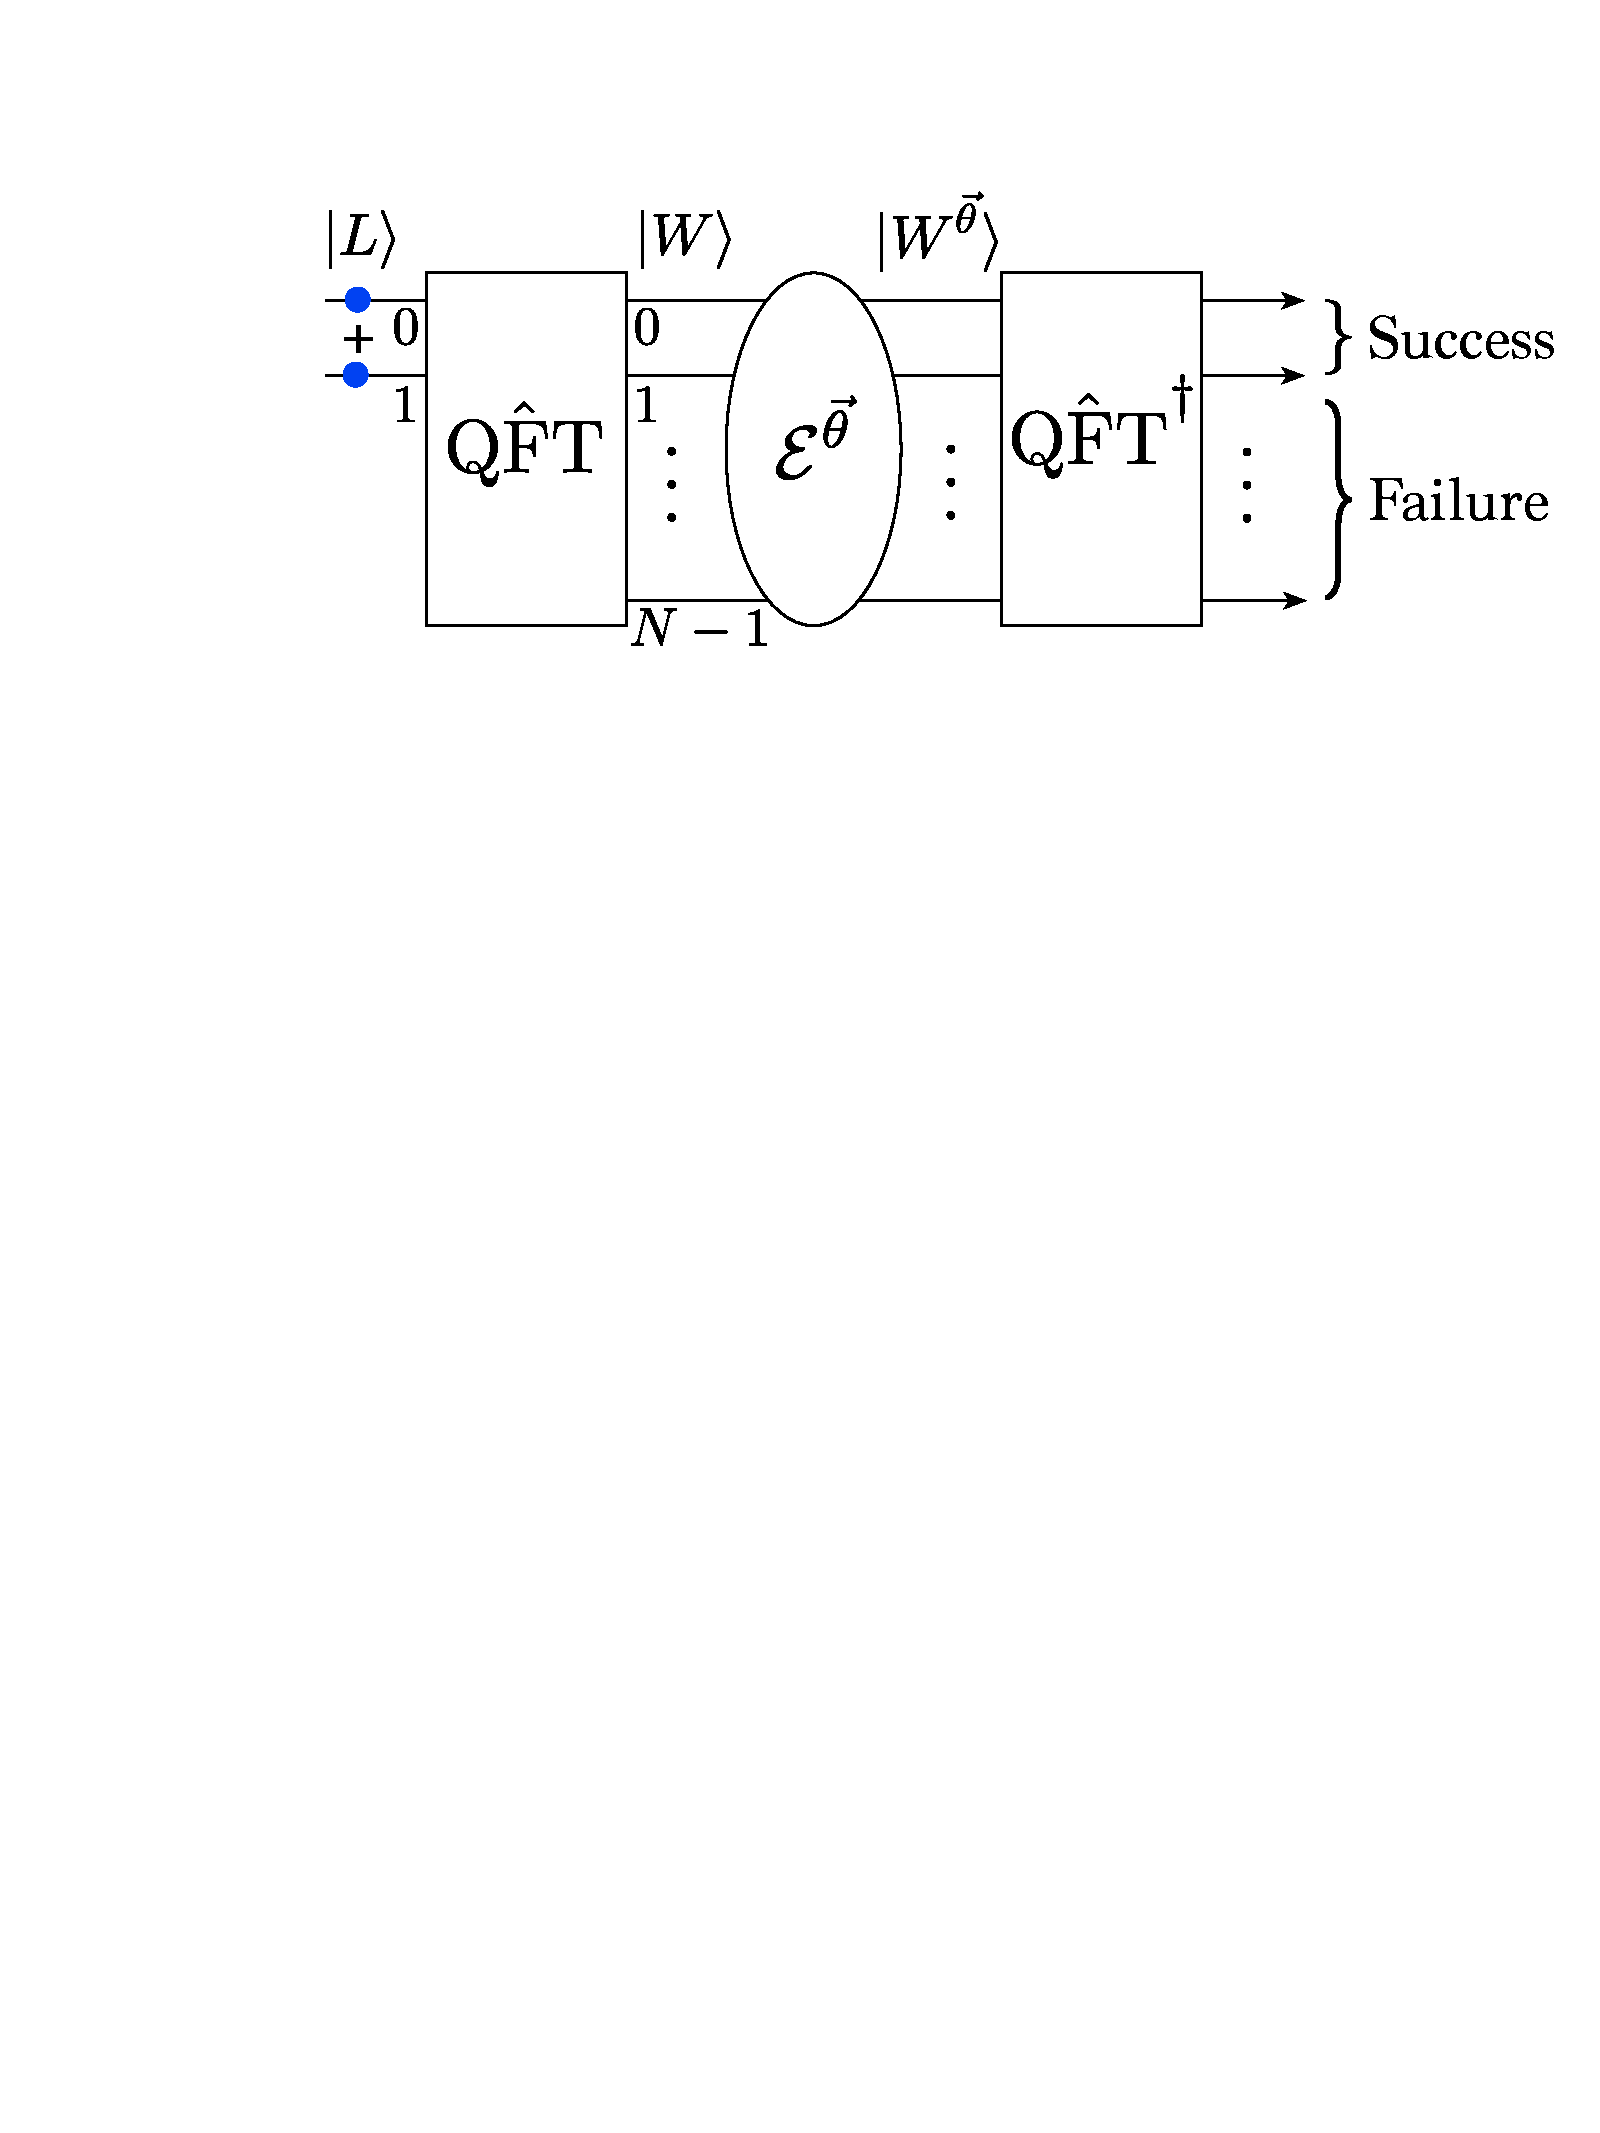
\includegraphics[width=0.475\textwidth]{W_state_memory}
	\caption{Quantum memory based on W-state encoding. Rails represent optical modes, and the input logical qubit state, $\ket{L}$, is represented using dual-rail encoding. The QFT fanout operation maps each of the two input basis states to one of two orthogonal $N$-qubit W-states, $\ket{W}$, differing only by their phase relationships. These are then fed into a bank of $N$ quantum memories. To readout the memories we convert back to optical encoding and decode using the inverse QFT operation. Success of the protocol is defined as there being exactly one photon between the first two `success' output modes. If a photon leaks into any of the other `failure' output modes we discard the state and assume it was erroneous. Thus error detection is heralded via the presence or absence of a photon in the `failure' modes.}\label{fig:W_state_memory}
\end{figure}

\comment{Show mathematical results}

%
% High-Level Protocols
%

\section{High-level protocols} \index{High-level protocols}

\dropcap{B}{uilding} upon the aforementioned primitive protocols for quantum networking, we can construct a plethora of higher-level protocols that implement more powerful end-user applications. These high-level protocols are ubiquitous in quantum information processing and form building blocks for even more powerful architectures, such as full cloud quantum computing, to be discussed in Sec.~\ref{sec:cloud}.

%
% Random Number Generation
%

\subsection{Random number generation} \index{Random number generation}

Perhaps the simplest quantum information processing task is that of perfect random number generation. True random numbers have widespread applications in cryptography, Monte-Carlo simulations, and any type of randomised (e.g \textbf{BPP}\index{BPP}) algorithm.

Classical random number generators are actually deterministic, but so difficult to predict that we accept them to be as good as random. But for some applications this isn't enough, and we must make sure that no correlations of any type exist between different random numbers, or between the random numbers and their environment.

This can be achieved in many different ways quantum mechanically. Ultimately, they are all based on the Heisenberg uncertainty principle, that certain quantum mechanical measurements yield uncertainty. The procedure is shown in Alg.~\ref{alg:random_number}.

\startalgtable
\begin{table}[!htbp]
\begin{mdframed}[innertopmargin=3pt, innerbottommargin=3pt, nobreak]
\texttt{
function RandomBit():
\begin{enumerate}
    \item Prepare the equal superposition state,
    \begin{align}
    \ket\psi_\mathrm{in} = \ket{+} = \frac{1}{\sqrt{2}}(\ket{0}+\ket{1}).
    \end{align}
    \item Most commonly this is in the polarisation basis,
    \begin{align}
    \ket{H}&\equiv\ket{0}, \nonumber \\
    \ket{V}&\equiv\ket{1}.
    \end{align}
    \item Measure the state in the logical basis, with measurement projectors,
    \begin{align}
    \hat\Pi_0 &= \ket{0}\bra{0}, \nonumber \\
    \hat\Pi_1 &= \ket{1}\bra{1}.
    \end{align}
    \item The measurement outcomes occur with probabilities,
    \begin{align}
    P_0&=|\langle 0|+\rangle|^2 = \frac{1}{2}, \nonumber \\
    P_1&=|\langle 1|+\rangle|^2 = \frac{1}{2},
    \end{align}
    following a uniform, random, binary distribution.
    \item Repeat for as many random bits as are required.
    \item $\Box$
\end{enumerate}}
\end{mdframed}
\captionspacealg \caption{Procedure for the generation of random bit-strings. Assuming the device is perfectly implementing this procedure, we will measure a perfect random 50/50 distribution between the two measurement outcomes. Note that the procedure requires no quantum interference, and no entanglement. Only single-qubit state preparation and measurement are required. Thus, a single-photon source, wave-plate, polarisation filter, and photo-detector are sufficient for its realisation. Favourably, if the detector is inefficient it simply reduces the bit-rate, but does not compromise the randomness of the distribution.} \label{alg:random_number}
\end{table}

The cynics amongst us might question the non-determinism\index{Non-determinism of quantum mechanics} of the laws of Nature (`God does not play dice!' -- Albert Einstein), and ask whether quantum random numbers really are truly random (in the sense of non-determinism), or whether they also are just too hard to predict that we treat them as effectively random. The answer to this is that it has been proven that quantum mechanics is inconsistent with `hidden variable theories' \cite{Bell}\index{Hidden variable theory}, i.e that there is an underlying, but inaccessible determinism in the world, which is guiding quantum measurements in a completely deterministic manner. This disproof effectively validates the notion of quantum mechanical perfect random number generation.

Consider the scenario where a client needs a stream of true random numbers for use in her Monte-Carlo simulation algorithm or as a secret key for her email encryption. She has limited quantum resources herself, so she outsources it to her better-equipped mate. Depending on her own resource limitations and potential security considerations, her friend could either: (1) implement the full protocol described above, providing her with a classical random bitstream; or (2) only take care of photon generation, providing her with a perpetual source of high-quality photons for her to measure herself using a simple photo-detector. (1) and (2) would both be suitable if the intention was to apply the source of randomness to a Monte-Carlo simulation. But in a cryptographic scenario, where the randomness is being used for key generation, clearly Alice could not outsource the measurement stage without revealing her secret key. In this instance, Bob can act as the provider of photons, while Alice does the measurements herself so as to keep her random bit-string secret.

This scenario is an obvious example of where a UDP-like \textsc{Send-and-forget} protocol may be viable. Unlike most other applications, Bob is broadcasting a stream of identical, pure quantum states, that are not entangled with any peripheral system, and are easily replicated, with no correlations between distinct photons. Thus, if any particular photon fails to reach Alice, it matters not, as she can simply await the next one emanating from Bob's bombardment of photons (the `shotgun' approach\index{Shotgun protocol}). There are no QoS requirements.

%
% Entanglement Purification
%

\subsection{Entanglement purification} \label{sec:ent_purif} \index{Entanglement purification}

Entangled states, most notably Bell pairs (Sec.~\ref{sec:bell_state_res}), play a central role in many quantum technologies. These maximally entangled states are easily represented optically using polarisation encoding of single photons, and can be non-deterministically prepared directly using SPDC (Sec.~\ref{sec:single_phot_src}), or post-selected linear optics \cite{???}.

Bell pairs are the basis for building cluster states (Sec.~\ref{sec:CSQC}), some quantum cryptography protocols (Sec.~\ref{sec:QKD}), and quantum teleportation (Sec.~\ref{sec:teleport}), to name just a few applications. Therefore distributing entangled states with the highest entanglement metrics is extremely important. In short, entanglement can be considered a valuable quantum resource (discussed in detail in Sec.~\ref{sec:ent_ultimate}), upon which many other protocols may be built.

Suppose Alice and Bob share an entangled pair. Quantum mechanics, specifically the very definition of entanglement itself, prohibits local operations performed by Alice and Bob from increasing the level of entanglement. However, if Alice and Bob share multiple pairs, they can perform an operation known as \textit{entanglement purification} or \textit{entanglement distillation}, whereby two lower-fidelity entangled pairs are consumed and projected onto a single entangled pair with higher fidelity \cite{bib:PRA_53_2046, bib:PRA_54_3824, bib:PRL_77_2818}. Such protocols will be extremely useful in protocols where achieving the highest possible degree of entanglement is paramount, for example when error thresholds must be achieved for the purpose of error-correction and fault-tolerance \cite{bib:NielsenChuang00}.

Taking two polarisation-encoded photonic Bell pairs, say $\ket{\Psi^+}$, and subjecting them to a dephasing error model (Sec.~\ref{sec:dephasing_error})\index{Dephasing channel} yields a mixed state of the form,
\begin{align}
\hat\rho_\mathrm{in} = F\ket{\Psi^+}\bra{\Psi^+} + (1-F)\ket{\Psi^-}\bra{\Psi^-},
\end{align}
where $F$ is the entanglement fidelity, which is a function of the dephasing rate. Note that $\ket{\Psi^+}$ and $\ket{\Psi^-}$ are related by local Pauli phase-flip operations ($\hat{Z}$) applied to either qubit,
\begin{align} \label{eq:psi_minus}
\ket{\Psi^-} = \hat{Z}_A \ket{\Psi^+} = \hat{Z}_B \ket{\Psi^+}.
\end{align}

A linear optics entanglement purification protocol can be simply implemented using two polarising beamsplitters PBSs \cite{bib:Pan01, bib:Pan03}. Alice uses one PBS to interfere the photons from her side of each of the photon pairs, measuring one output only, which implements a non-deterministic, partial Bell state projection. Bob does the same on his side. What's left is one photon in Alice's hands and one in Bob's. When successful, they will now be sharing a single entangled pair of higher Bell state fidelity than the two starting states. The protocol is shown in Fig.~\ref{fig:ent_purif_prot}.

Note that when using PBSs to perform the Bell projections, the protocol is necessarily non-deterministic, since PBSs are only able to distinguish two of the four Bell states. Thus, each PBS has a success probability of $1/2$. And there are two PBSs per instance of the protocol, therefore the net success probability is $1/4$. When concatenated, $n$ applications of the protocol thus has an exponentially low success probability of $1/4^n$. This could be overcome using deterministic CNOT gates (Sec.~\ref{sec:KLM_univ}), but these are challenging using linear optics.

Furthermore, the protocol consumes two Bell pairs upon each trial, only one quarter of which are successful. Thus, on average, 8 Bell pairs are consumed for every purified Bell pair prepared, and the expected number of Bell pairs required to perform $n$ iterations of entanglement purification grows exponentially as $8^n$.

\begin{figure}[!htbp]
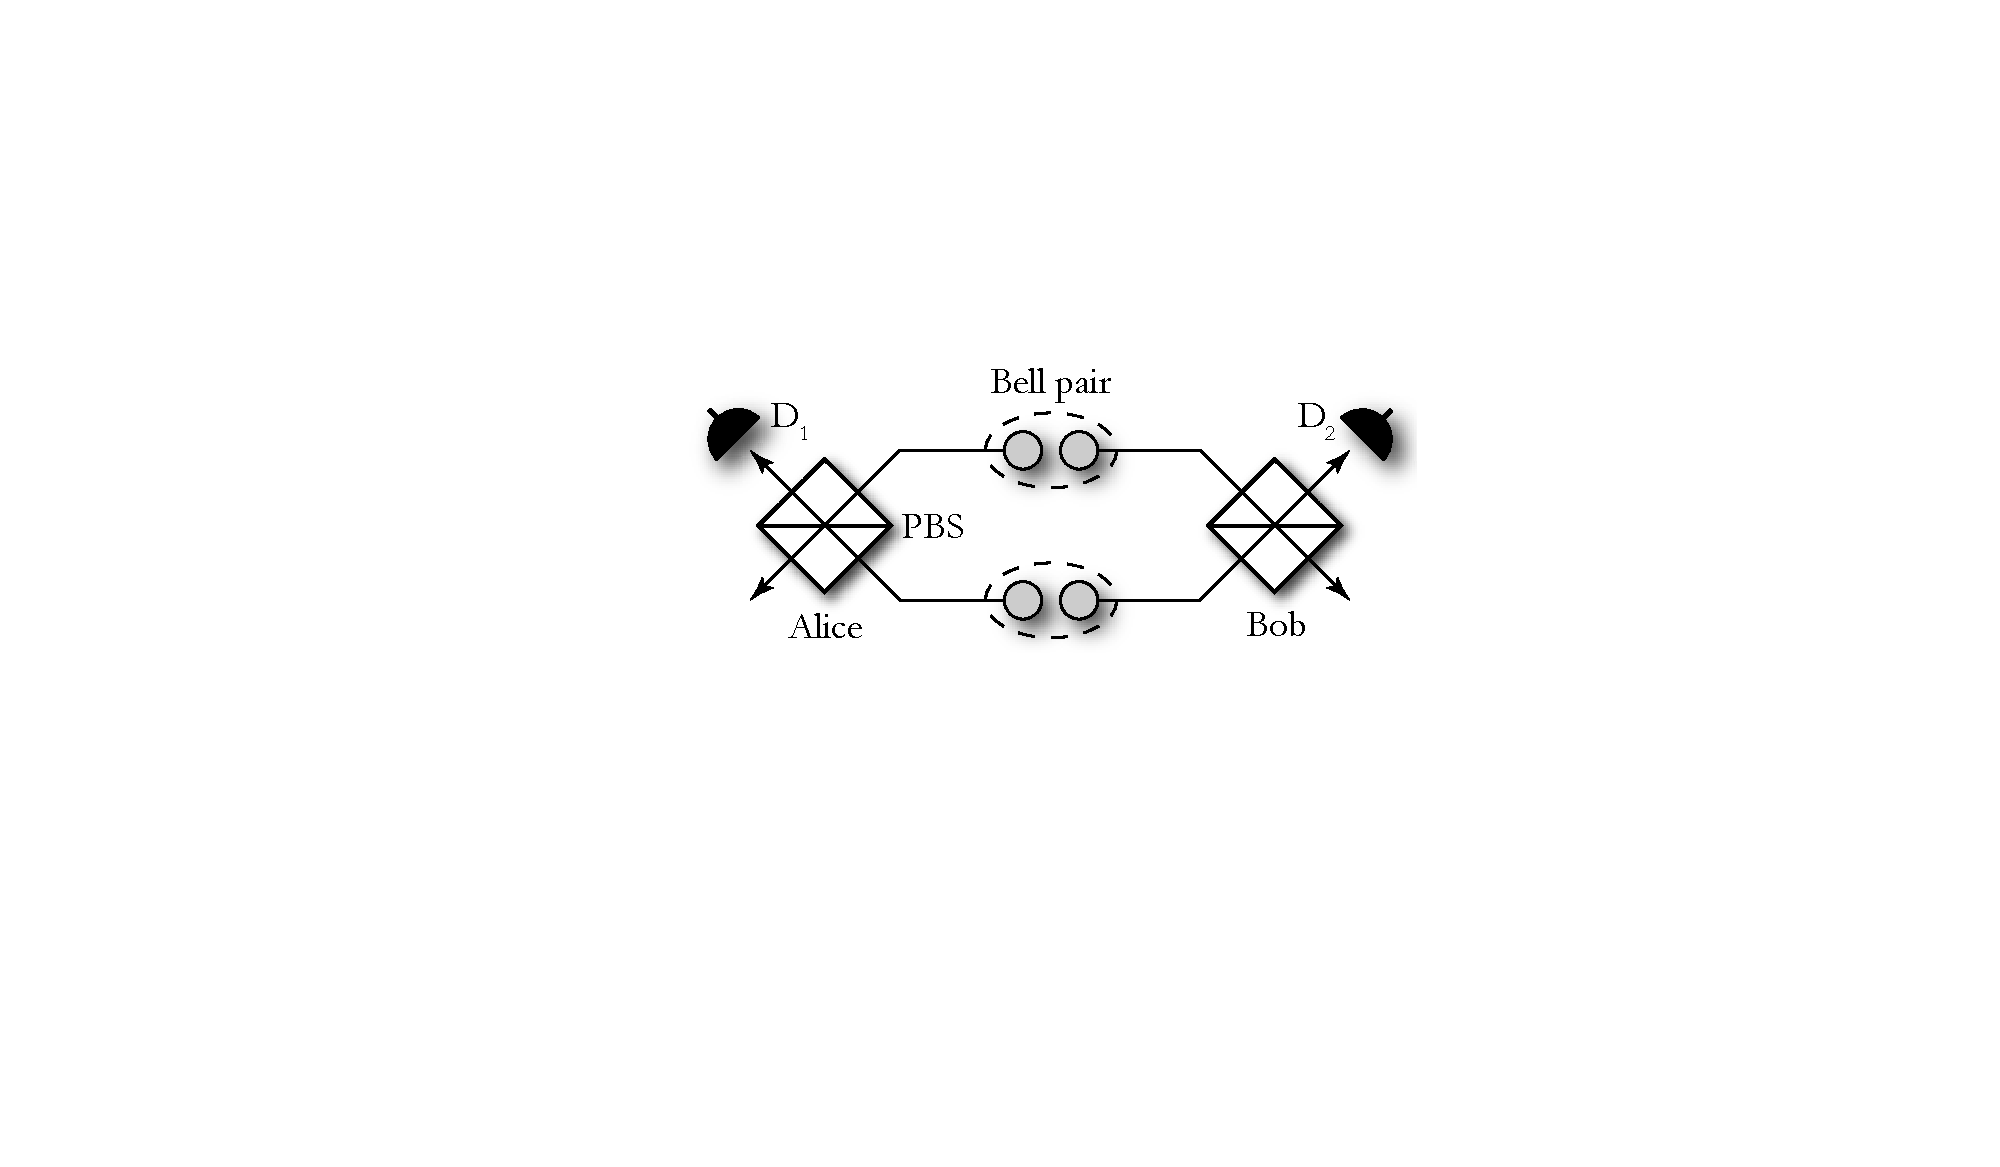
\includegraphics[clip=true, width=0.45\textwidth]{ent_purif_prot}
\captionspacefig \caption{Elementary entanglement purification using linear optics. Two Bell pairs are distributed between Alice and Bob, each of which has been subject to a dephasing error model. Alice and Bob perform Bell measurements on their two qubits using a PBS and polarisation-resolved photo-detection ($D_1$ and $D_2$). Upon successful Bell state projection (Bell measurements are necessarily non-deterministic using linear optics), Alice and Bob will share a single Bell pair with higher fidelity than the two input pairs.} \label{fig:ent_purif_prot}
\end{figure}

Specifically, the relationship between the input ($F_\mathrm{in}$) and output ($F_\mathrm{out}$) fidelities of the protocol is,
\begin{align}
F_\mathrm{out} = \frac{{F_\mathrm{in}}^2}{{F_\mathrm{in}}^2 + (1-F_\mathrm{in})^2}.
\end{align}
This input/output relationship is shown in Fig.~\ref{fig:ent_purif}.

\begin{figure}[!htbp]
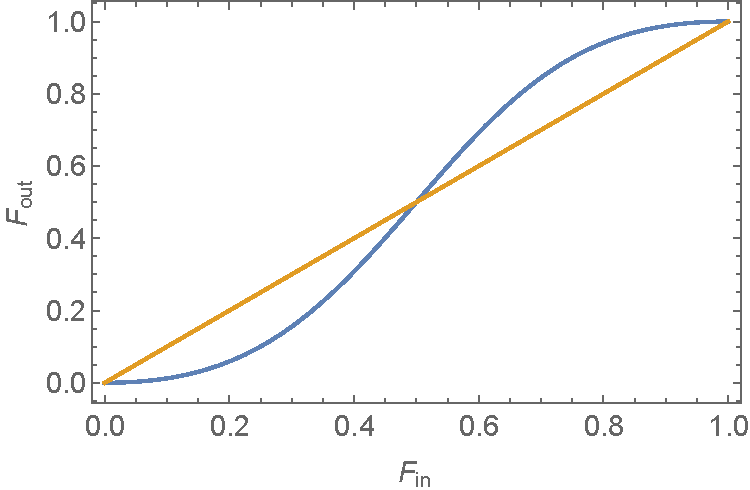
\includegraphics[clip=true, width=0.475\textwidth]{ent_purif}
\captionspacefig \caption{Entanglement purification of two polarisation-encoded, photonic Bell pairs. $F_\mathrm{in}$ ($F_\mathrm{out}$) are the input (output) fidelities of the Bell pairs. The protocol consumes two Bell pairs for every one purified pair. The straight line represents the break-even point in terms of state fidelity, above which the protocol enhances fidelity, and below which reduces it. This places a strict bound on the fidelity of Bell pairs reaching the purifier. This equates to route cost, if measured by the fidelity metric, stipulating network performance requirements. This threshold requirement presents an example of where an \textsc{All or Nothing} strategy might be appropriate.} \label{fig:ent_purif}
\end{figure}

Note that there is a break-even point, above which the protocol strictly increases fidelity, and below which strictly decreases it. This occurs at \mbox{$F_\mathrm{in}=1/2$}. Provided pairs can be communicated above this fidelity threshold, bootstrapped application of the protocol could be employed to boost entanglement fidelity asymptotically close to unity (but with exponential resource overhead, since each operation non-deterministically consumes two pairs to produce one). But below this threshold it is impossible to recover any more entanglement than we started with. This provides an example of an application where the protocol being implemented dictates strict requirements on network cost metrics. Specifically, assuming perfect Bell pairs to begin with, the routes by which they are communicated must strictly ensure entanglement fidelities of at least \mbox{$F=1/2$} upon reaching their destination. Here a type of \textsc{All or Nothing} networking strategy would be applicable -- if the fidelity requirement is not met, the state cannot be purified and might as well be thrown away to make way for other traffic.

A theoretical analysis of this protocol has been performed, accounting for mode-mismatch (Sec.~\ref{sec:MM_error}) in the protocol \cite{bib:RohdeOptEntPur06}, where it was found that mode-mismatch shifts the break-even point upwards, and lowers the maximum value of $F_\mathrm{out}$ -- with more mode-mismatch, a higher starting fidelity is required to break even, and we achieve a lower, sub-unity output fidelity. In this case, a cost function that combines the dephasing and mode-mismatch metrics of the network will be required.

Importantly, this protocol is based on partial Bell state measurement, and therefore does not require interferometric stability, only high HOM visibility, thus making stabilisation comparatively easy over long distances.

Entanglement purification can also be performed using physical encodings other than single photons. For example, this has been demonstrated using Gaussian CV quantum states \cite{bib:Duan00}.

%
% Quantum State Teleportation
%

\subsection{Quantum state teleportation} \label{sec:teleport} \index{Quantum state teleportation}

Quantum state teleportation \cite{???, bib:PRL_70_1895} is an essential ingredient in many higher-level protocols. It forms the basis of cluster state quantum computing (Sec.~\ref{sec:CSQC}), some QEC codes, the KLM linear optics quantum computing scheme (Sec.~\ref{sec:KLM_univ}), and can act as a mediator for long-range transmission of quantum states, amongst others.

In the standard teleportation protocol, Alice begins with a single qubit,
\begin{align}
\ket\phi = \alpha\ket{0} +\beta\ket{1},
\end{align}
which she would like to teleport to Bob. Importantly, no quantum communication between the two is allowed, since obviously this would make the problem trivial. However, classical communication is allowed (and turns out to be necessary), and furthermore they share an entangled Bell pair as a resource. Thus, Alice begins with two qubits, and Bob begins with one -- his half of the entangled pair onto which Alice's state ought to be teleported. The initial state is therefore,
\begin{align}
\ket\psi_\mathrm{in} &= \ket{\phi}_{A_1} \ket{\Psi^+}_{A_2,B} \\
&= \frac{1}{\sqrt{2}} (\alpha\ket{0}_{A_1}+\beta\ket{1}_{A_1}) (\ket{0}_{A_2}\ket{1}_B + \ket{1}_{A_2}\ket{0}_B). \nonumber
\end{align}

The first step of the protocol is for Alice to perform a 2-qubit entangling measurement on her two qubits, projecting onto the Bell basis [Eq.~(\ref{eq:bell_basis})]. She obtains one of four measurement outcomes. For illustration, suppose she measures the $\ket{\Psi^+}$ outcome. Then the projected state is,
\begin{align}
\ket\psi_\mathrm{proj}^{\Psi^+} &= \bra{\Psi^+}_{A_1,A_2} \ket\psi_\mathrm{in} \nonumber \\
&= \frac{1}{\sqrt{2}} \bra{\Psi^+}_{A_1,A_2}\ket\psi_{A_1}(\ket{0}_{A_2}\ket{1}_B + \ket{1}_{A_2}\ket{0}_B) \nonumber \\
&= \frac{1}{2} (\bra{0}_{A_1}\bra{1}_{A_2} + \bra{1}_{A_1}\bra{0}_{A_2}) \nonumber \\
&\cdot (\alpha\ket{0}_{A_1}+\beta\ket{1}_{A_1})(\ket{0}_{A_2}\ket{1}_B + \ket{1}_{A_2}\ket{0}_B) \nonumber \\
&= \frac{1}{2} (\alpha \ket{0}_B + \beta \ket{1}_B)\nonumber \\
&= \frac{1}{2} \ket\phi_B,
\end{align}
which is Alice's initial state. For all four possible Bell measurement outcomes we have,
\begin{align}
\ket\psi_\mathrm{proj}^{\Psi^+} &= \frac{1}{2} (\alpha \ket{0}_B + \beta \ket{1}_B) \nonumber \\
&= \frac{1}{2} \ket\phi_B, \nonumber \\
\ket\psi_\mathrm{proj}^{\Psi^-} &= \frac{1}{2} (\alpha \ket{0}_B - \beta \ket{1}_B) \nonumber \\
&= \frac{1}{2} \hat{Z}\ket\phi_B, \nonumber \\
\ket\psi_\mathrm{proj}^{\Phi^+} &= \frac{1}{2} (\alpha \ket{1}_B + \beta \ket{0}_B) \nonumber \\
&= \frac{1}{2} \hat{X} \ket\phi_B, \nonumber \\
\ket\psi_\mathrm{proj}^{\Phi^-} &= \frac{1}{2} (\alpha \ket{1}_B - \beta \ket{0}_B) \nonumber \\
&= \frac{1}{2} \hat{X}\hat{Z}\ket\phi_B,
\end{align}
which are all locally equivalent to $\ket\phi$ under Pauli gates, and can be corrected by Bob, given communication of the classical Bell measurement outcome provided by Alice. The full protocol is described in Alg.~\ref{alg:state_teleport}.

\begin{table}[!htbp]
\begin{mdframed}[innertopmargin=3pt, innerbottommargin=3pt, nobreak]
\texttt{
function StateTeleportation($\ket\phi_{A_1}$, $\ket{\Phi^+}_{A_2,B}$):
\begin{enumerate}
    \item Alice prepares the state $\ket\phi_{A_1}$, which she would like to teleport to Bob.
    \item Alice and Bob share the Bell pair $\ket{\Phi^+}_{A_2,B}$.
    \item Alice performs a Bell state projection between qubits $A_1$ and $A_2$.
    \item Alice communicates the classical measurement outcome to Bob - one of four outcomes.
    \item Bob applies an appropriate local correction to his qubit - some combination of the Pauli operators $\hat{X}$ and $\hat{Z}$ - according to the classical measurement outcome:
    \begin{align}
    \ket{\Psi^+}\bra{\Psi^+} &\to \hat{\mathbb{I}}, \nonumber \\
    \ket{\Psi^-}\bra{\Psi^-} &\to \hat{Z}, \nonumber \\
    \ket{\Phi^+}\bra{\Phi^+} &\to \hat{X}, \nonumber \\
    \ket{\Phi^-}\bra{\Phi^-} &\to \hat{Z}\hat{X}.
    \end{align}
    \item Bob is left with the state $\ket\phi_B$.
    \item $\Box$
\end{enumerate}}
\begin{align}
\Qcircuit @C=1em @R=1.6em {
    \lstick{\ket\phi} & \qw & \multimeasureD{1}{\mathrm{Bell}} & \cw  & \control \cw \\
    \lstick{} & \qw & \ghost{\mathrm{Bell}} & \control \cw & \cwx \\
    \lstick{} & \qw & \qw & \gate{X} \cwx & \gate{Z} \cwx & \qw & \qw & \ket\phi
    \inputgroupv{2}{3}{.8em}{.8em}{\ket{\Phi^+}}
} \nonumber
\end{align}
\end{mdframed}
\captionspacealg \caption{Quantum state teleportation of a single qubit.} \label{alg:state_teleport}
\end{table}

In general, the protocol is deterministic, although using PBSs to perform partial Bell measurements, the success probability is at most $1/2$.

The question now is what error metrics apply and how do they accumulate in the teleportation protocol. The answer is straightforward -- the final teleported qubit accumulates all local Pauli errors (e.g dephasing or depolarisation) associated with Alice's input state as well as any that acted upon the shared Bell pair. That is, the errors get teleported along with the state being teleported, plus any errors on the Bell pair.

In the case of loss, loss of either of Alice's qubits will immediately be detected when she performs her Bell measurement. Thus, loss becomes a located error, and the knowledge of the error allows the associated packet to be discarded, and the sender and recipient notified. On the other hand, loss of Bob's qubit will behave no differently than loss acting on an ordinary qubit channel.

Thus, in terms of Pauli errors, no special treatment is required by the QTCP protocol -- it is almost as if the teleportation protocol weren't there. And in terms of loss, the Bell state projection diagnoses lost qubits, allowing appropriate action to be taken, which is actually better than if the error were undiagnosed. These are often referred as \textit{located}\index{Located errors} and \textit{unlocated}\index{Unlocated errors} errors.

The total resources required to teleport a single-qubit state are:
\begin{enumerate}
\item The qubit to be teleported.
\item A shared Bell pair.
\item A 2-qubit entangling measurement in the Bell basis.
\item The transmission of two classical bits.
\item Two classically-controlled Pauli gates for correction.
\end{enumerate}

This is more costly than sending the qubit directly over a quantum channel, but may be the only approach if a direct link is not available. In the context of an internet where entanglement distribution is treated as the fundamental resource (Sec.~\ref{sec:ent_ultimate}), state teleportation is the natural approach for communicating quantum states, since no quantum communication of any kind is required once the two parties have a shared Bell pair between them.

The important feature of this protocol to note is that there is no direct quantum communication between Alice and Bob, only a classical communications channel. Rather, the Bell pair mediates the transfer of quantum information, despite there being no direct quantum channel between Alice and Bob.

Relying on teleportation rather than direct quantum communication makes frugal use of quantum channels, since there is no need for direct quantum routes between every pair of nodes in the network. Instead, each node need only have a direct one-way quantum link with the central authority responsible for entanglement distribution, thereby significantly reducing the complexity of the topology of the quantum network.

The Bell state measurement can be implemented either using a CNOT gate, or as a non-deterministic partial Bell state measurement using a PBS (Sec.~\ref{sec:bell_proj}), both of which are non-deterministic using purely linear optics.

The above describes quantum state teleportation at the level of single qubits. However, when dealing with more general QTCP packets, which may have multi-qubit payloads, we may wish to teleport an entire packet\index{Packet teleportation}. This is implemented as a simple extension of the above procedure -- we simply implement $n$ multiple independent teleportation protocols to all of the packet's $n$ constituent qubits. Via linearly, although the teleportation protocols are being applied independently to each qubit, the net packet teleportation operation will preserve their joint state, including entanglement between them. Note, however, that if the qubit state teleportation protocols are individually non-deterministic with success probability $p_\mathrm{teleport}$, the net success probability for the teleportation of the entire packet scales inverse exponentially with $n$, as ${p_\mathrm{teleport}}^n$.

%
% Quantum Gate Teleportation
%

\subsection{Quantum gate teleportation} \label{sec:teleport_gate} \index{Quantum gate teleportation}

Using quantum \textit{state} teleportation as a primitive building block, quantum \textit{gate} teleportation may be implemented \cite{bib:GottesmanChuang99}. Here rather than teleporting a quantum state from one physical system to another, we teleport the action of a quantum gate onto a physical system (archetypically a maximally entangling 2-qubit gate, such as a CNOT gate).

The general outline of the derivation of the protocol for teleporting a CNOT gate onto a 2-qubit state is shown in Alg.~\ref{alg:gate_teleport}.

\begin{table}[!htbp]
\begin{mdframed}[innertopmargin=3pt, innerbottommargin=3pt, nobreak]
\texttt{
function GateTeleportation($\ket\psi_A\ket\phi_B$):\
\begin{enumerate}
\item We wish to apply a CNOT gate to \mbox{$\ket\psi_{A}\ket\phi_{B}$}.
\item Introduce two additional qubits, $C$ and $D$.
\item Teleport states \mbox{$\ket\psi_{A}\to\ket\psi_C$}, \mbox{$\ket\psi_{B}\to\ket\psi_D$}.
\item Apply \mbox{$\hat{\mathrm{CNOT}} \ket \psi_C \ket\phi_D$}.
\begin{align}
\Qcircuit @C=1em @R=1.6em {
\lstick{\ket\psi} & \qw & \multimeasureD{1}{\mathrm{Bell}} & \cw  & \control \cw \\
\lstick{} & \qw & \ghost{\mathrm{Bell}} & \control \cw & \cwx \\
\lstick{} & \qw & \qw & \gate{X} \cwx & \gate{Z} \cwx & \ctrl{1} & \qw & \qw & \qw \inputgroupv{2}{3}{.8em}{.8em}{\ket{\Phi^+}} \\
\lstick{} & \qw & \qw & \gate{X} & \gate{Z} & \targ & \qw & \qw & \qw \inputgroupv{4}{5}{.8em}{.8em}{\ket{\Phi^+}} \\
\lstick{} & \qw & \multimeasureD{1}{\mathrm{Bell}} & \control \cw \cwx & \cwx \\
\lstick{\ket\phi} & \qw & \ghost{\mathrm{Bell}} & \cw  & \control \cw \cwx
} \nonumber
\end{align}
\item The CNOT is a Clifford gate and can therefore be commuted to the front of the Pauli operators to yield a CNOT followed by some different configuration of Pauli operators.
\item The CNOT now acts jointly upon the Bell pairs that were acting as a resource for the state teleportation, independent of \mbox{$\ket\psi_{A}\ket\phi_{B}$}.
\item Group the CNOT gate and Bell pairs together, and treat them as a 4-qubit resource state preparation stage, which does not depend on \mbox{$\ket\psi_{A}\ket\phi_{B}$}. 
\item Prepare the 4-qubit resource state, \mbox{$\ket\chi=\hat{\mathrm{CNOT}}_{2,3}\ket{\Psi^+}_{1,2}\ket{\Psi^+}_{3,4}$}, offline in advance.
\item If the CNOT is non-deterministic, employ \textsc{Repeat Until Success} to prepare $\ket\chi$.
\item The output state is \mbox{$\hat{\mathrm{CNOT}}_{C,D} \ket\psi_{C}\ket\phi_{D}$}.
\item $\Box$
\end{enumerate}}
\begin{align}
\Qcircuit @C=1em @R=1.6em {
\lstick{\ket\psi} & \qw & \multimeasureD{1}{\mathrm{Bell}} & \cw & \cw & \control \cw \\
\lstick{} & \qw & \ghost{\mathrm{Bell}} & \cw & \cw & \cw \cwx & \control \cw \\
\lstick{} & \qw & \qw & \gate{X} & \gate{Z} & \qw \cwx & \gate{Z} \cwx & \qw & \qw & \qw \\
\lstick{} & \qw & \qw & \gate{X} \cwx & \qw \cwx & \gate{X} \cwx & \gate{Z} \cwx & \qw & \qw & \qw \\
\lstick{} & \qw & \multimeasureD{1}{\mathrm{Bell}} & \control \cw \cwx & \cwx \inputgroupv{2}{5}{0.8em}{4.1em}{\ket{\chi}} \\
\lstick{\ket\phi} & \qw & \ghost{\mathrm{Bell}} & \cw  & \control \cw \cwx
} \nonumber
\end{align}
\end{mdframed}
\captionspacealg \caption{Teleporting a CNOT gate onto a 2-qubit state.} \label{alg:gate_teleport}
\end{table}

Most notably, gate teleportation is useful when attempting to apply 2-qubit entangling operations using non-deterministic gates, in which case gate teleportation allows the non-deterministic elements to be performed offline as a resource state preparation stage, overcoming the non-determinism during the gate application stage.

Specifically, when a CNOT gate acting directly upon two qubits fails, it corrupts those qubits, whereas if it fails during a state preparation stage, it can simply be reattempted until a success occurs, without corrupting the target qubits. A concatenated version of the gate teleportation protocol forms the basis for constructing near-deterministic entangling gates in linear optics, to be explained in detail in Sec.~\ref{sec:KLM_univ}.

Quantum gate teleportation effectively reduces the problem of implementing CNOT gates to:
\begin{enumerate}
\item Offline preparation of highly-entangled 4-qubit resource states. This needn't be deterministic, since the resource state does not depend on the state to which the CNOT gate ought to be applied.
\item Two Bell measurements.
\item Some configuration of local Pauli operators, dependent upon the Bell measurement outcomes.
\end{enumerate}
Importantly, like quantum state teleportation, there is no need for a quantum communications channel between the two parties holding the qubits to which the gate is applied -- classical communication is sufficient.

The gate teleportation idea is conceptually interesting as it converts the problem of `gate application' to that of `state preparation'\footnote{The resource state is prepared from two Bell pairs and a single CNOT gate, which is locally equivalent to a 4-qubit GHZ state. In the absence of a direct source of Bell pairs, they can be prepared using separable single-qubit states and a CNOT gate. Thus, the full resource state may be prepared from separable single qubits via three CNOT gates.}, by commuting all the entangling operations to the beginning of the protocol. Cluster state quantum computing (Sec.~\ref{sec:CSQC}) is actually the extremity of this logic, whereby an entire quantum computation is transformed into a sequence of state and gate teleportations. One may interpret this to mean that teleportation is a universal resource for quantum computation \cite{bib:GottesmanChuang99}.

The resource states required for gate teleportation are highly-entangled 4-qubit states, which are challenging to prepare, especially in the optical context. Thus, as with cluster states, if the preparation of these resource states were to be outsourced to a specialised provider, they could be in high demand.

Note that this technique works for the CNOT gate because it is a Clifford gate\index{Clifford gates} (i.e it commutes with the classically-controlled Pauli gates to yield a different combination of classically-controlled Pauli gates). Thus, this technique does not automatically apply to \textit{any} 2-qubit gate.

%
% Entanglement Swapping
%

\subsection{Entanglement swapping} \label{sec:swapping} \index{Entanglement swapping}

The obvious approach to sending a qubit from Alice to Bob is to send a qubit from Alice to Bob (duh!). However, over long distances this may accrue impractical error rates, particularly losses. The other alternative is to employ the quantum state teleportation protocol (Sec.~\ref{sec:teleport}) to teleport the state between the two parties. However, this requires that Alice and Bob first share an entangled Bell pair, which must itself be distributed across the same distances. Entanglement swapping \cite{???, bib:PRL_71_4287} is the process of taking two Bell pairs, one held by each party, and swapping the entanglement between them such that the two parties share an entangled state. This procedure can be bootstrapped to progressively swap the entanglement over longer and longer distances, yielding \textit{quantum repeater networks} (Sec.~\ref{sec:rep_net}). The procedure for this protocol is shown in Alg.~\ref{alg:ent_swap} and Fig.~\ref{fig:ent_swap}

\begin{table}[!htbp]
\begin{mdframed}[innertopmargin=3pt, innerbottommargin=3pt, nobreak]
\texttt{
function EntanglementSwapping($\ket{\Phi^+}^{\otimes 2}$):
\begin{enumerate}
    \item Alice locally prepares the Bell pair,
    \begin{align}
    \ket{\Phi^+}_{A_1,A_2}.
    \end{align}
    \item Bob locally prepares the Bell pair,
    \begin{align}
    \ket{\Phi^+}_{B_1,B_2}.
    \end{align}
    \item The net initial state is,
    \begin{align}
    \ket\psi_\mathrm{in} = \ket{\Phi^+}_{A_1,A_2} \ket{\Phi^+}_{B_1,B_2}.
    \end{align}
    \item Alice sends qubit $A_1$ to third party Eve.
    \item Bob sends qubit $B_1$ to third party Eve.
    \item Eve performs a Bell projection between $A_1$ and $B_1$, yielding,
    \begin{align}
    \bra{\Phi^+}_{A_1,B_1} \ket\psi_\mathrm{in} = \ket{\Phi^+}_{A_2,B_2}.
    \end{align}
    \item In the case of the other Bell projection outcomes ($\bra{\Phi^-}_{A_1,B_1}$, $\bra{\Psi^+}_{A_1,B_1}$ or $\bra{\Psi^-}_{A_1,B_1}$), local corrections (Pauli operators) are made by Alice and/or Bob, as dictated by classical communication from Eve,
    \begin{align}
    \bra{\Phi^+}_{A_1,B_1} \ket\psi_\mathrm{in} &= \ket{\Phi^+}_{A_2,B_2}, \nonumber \\
    \bra{\Phi^-}_{A_1,B_1} \ket\psi_\mathrm{in} &= \hat{Z}_{B_2} \ket{\Phi^+}_{A_2,B_2}, \nonumber \\
    \bra{\Psi^+}_{A_1,B_1} \ket\psi_\mathrm{in} &= \hat{X}_{B_2} \ket{\Phi^+}_{A_2,B_2}, \nonumber \\
    \bra{\Psi^-}_{A_1,B_1} \ket\psi_\mathrm{in} &= \hat{X}_{B_2} \hat{Z}_{B_2} \ket{\Phi^+}_{A_2,B_2}.
    \end{align}
    \item Alice and Bob now possess a joint Bell pair between qubits $A_2$ and $B_2$,
    \begin{align}
    \ket\psi_\mathrm{out} = \ket{\Phi^+}_{A_2,B_2}.
    \end{align}
    \item $\Box$ \\
\end{enumerate}}
\begin{align}
\Qcircuit @C=1em @R=1.6em {
    \lstick{} & \qw & \qw & \qw & \qw & \qw & \qw \\
    \lstick{} & \qw & \multimeasureD{1}{\mathrm{Bell}} & \cw  & \control \cw
    \inputgroupv{1}{2}{.8em}{.8em}{\ket{\Phi^+}} \\
    \lstick{} & \qw & \ghost{\mathrm{Bell}} & \control \cw & \cwx \\
    \lstick{} & \qw & \qw & \gate{X} \cwx & \gate{Z} \cwx & \qw & \qw
    \inputgroupv{3}{4}{.8em}{.8em}{\ket{\Phi^+}}
} \nonumber
\end{align}
\end{mdframed}
\captionspacealg \caption{Entanglement swapping protocol between two parties. Two Bell pairs held locally by two users, \mbox{$\ket{\Phi^+}_{A_1,A_2}\ket{\Phi^+}_{B_1,B_2}$}, are converted to a single Bell pair shared between the users, $\ket{\Phi^+}_{A_2,B_2}$.} \label{alg:ent_swap}
\end{table}

\begin{figure}[!htbp]
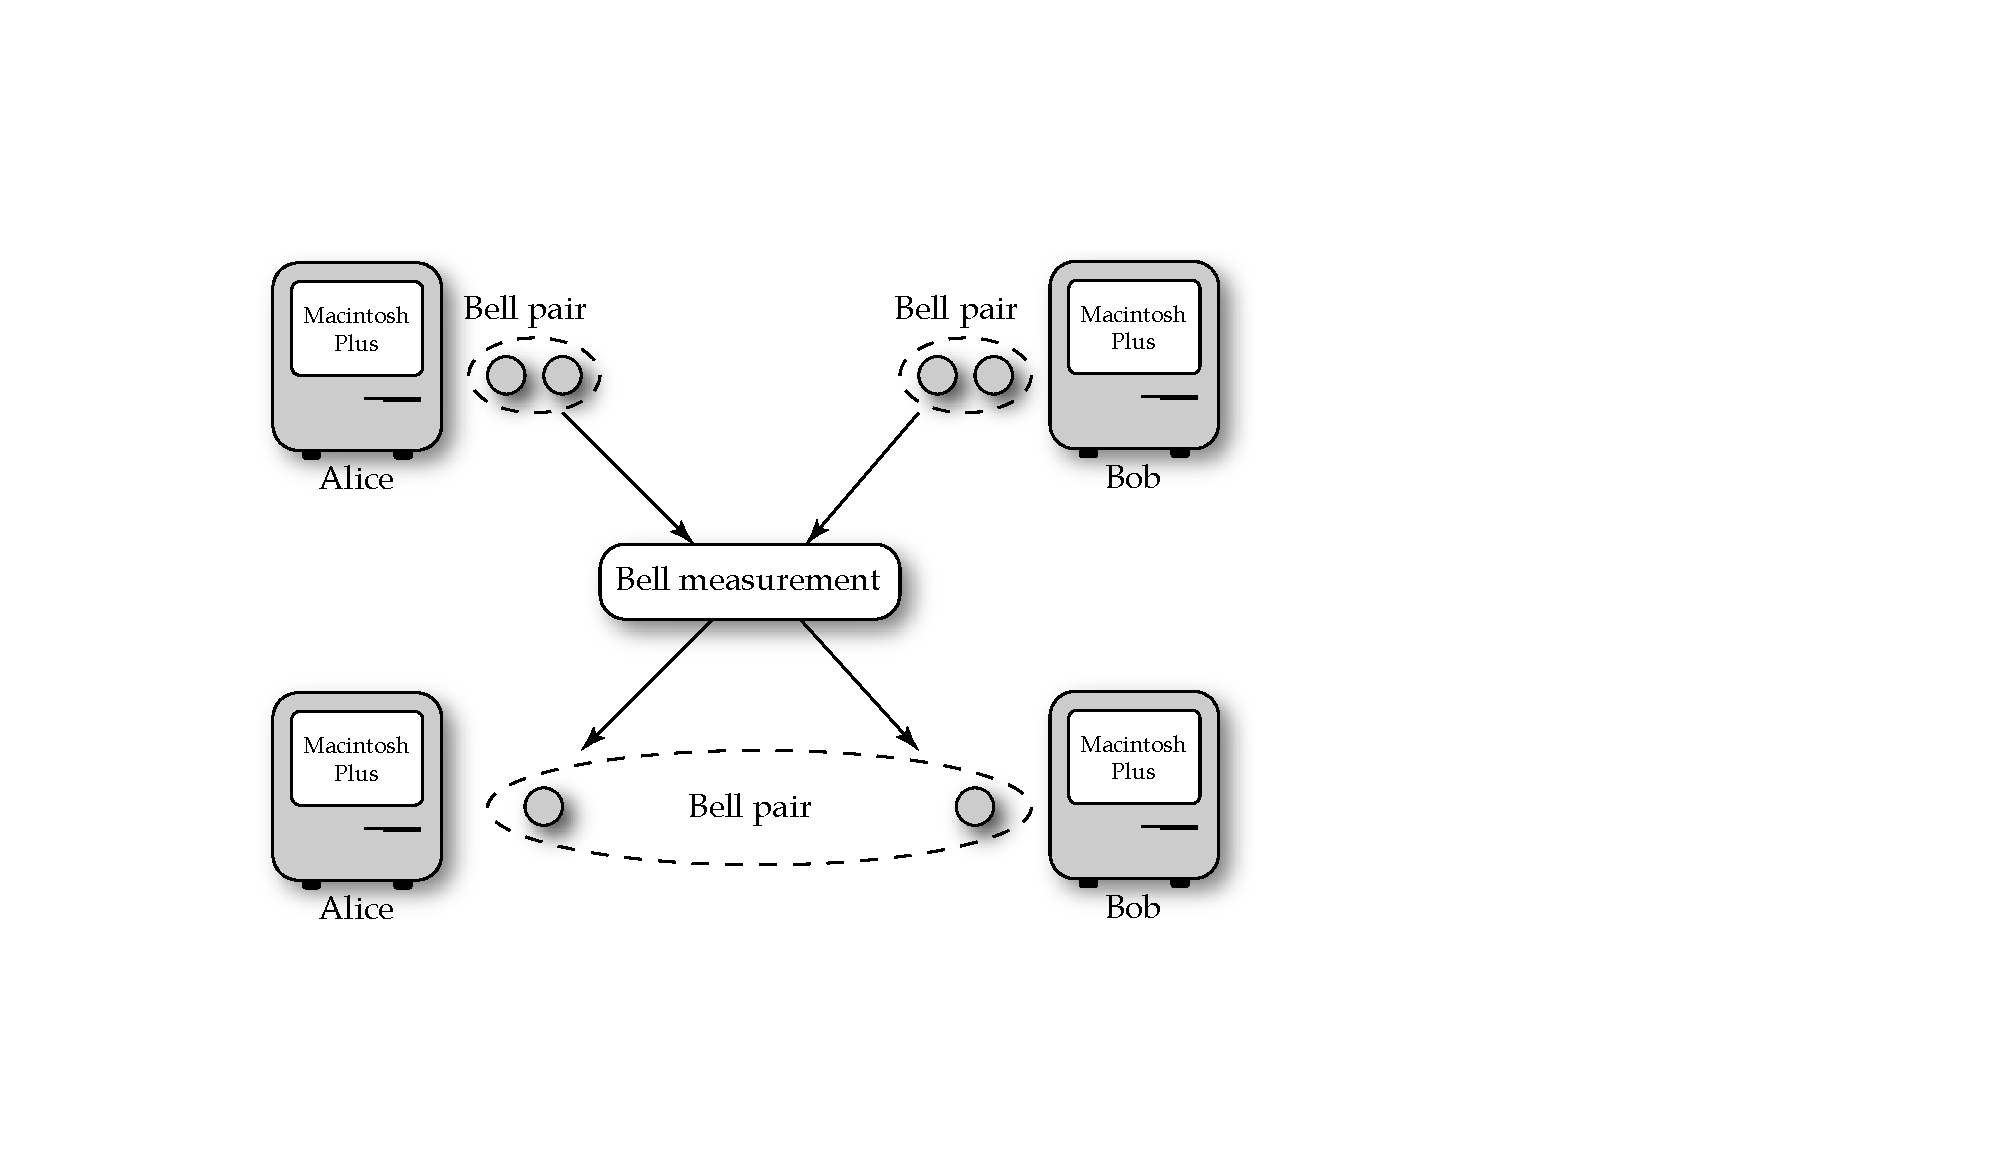
\includegraphics[clip=true, width=0.475\textwidth]{ent_swap}
\captionspacefig \caption{Entanglement swapping between two nodes. Each node initially holds a Bell pair (dotted ellipses) comprising two qubits (grey circles). One qubit from each pair is sent to the repeater between them, which measures them in the Bell basis. After local unitary corrections, the two nodes share an entangled pair.} \label{fig:ent_swap}
\end{figure}

In a sense, entanglement swapping can be regarded as `indirect' entanglement distribution, whereby entanglement is created between two distant parties who do not directly exchange any quantum information.

Alternately, note that the entanglement swapping is structurally almost identical to two instances of quantum state teleportation side-by-side. This is not a coincidence, and entanglement swapping can indeed be thought of as Bell pair state teleportation.

Now if instead of Alice and Bob we have a long chain of these operations in series, then the entanglement can be swapped across the entire length of the chain, enabling the preparation of end-to-end entangled pairs, which can be employed for state teleportation.

The advantage to this approach is that the range of each repeater can be much smaller than the entire length of the channel, easing constraints imposed by errors, notably loss. Furthermore, the entanglement swapping needn't be actually performed in any chronologically linear sequence. The operations could be arbitrarily ordered, since the measurements are independent and commute. Thus, if some segments are detected as failing (e.g qubits are lost), just those segments can be performed again without requiring the entire protocol to start from scratch, unlike the na{\" i}ve direct communication technique. This \textsc{Divide and Conquer} approach can drastically improve performance of the network in terms of channel capacity, improving the exponential dependence of loss on distance. 

The protocol is conceptually very similar to teleportation, where instead of teleporting a qubit state, we are teleporting entanglement. Because of this similarity, it inherits similar error propagation characteristics as for teleportation discussed previously. That is, errors acting on the qubits upon which the Bell measurements are performed are effectively teleported onto the remaining qubits. Then, entanglement purification can be implemented as a higher-level layer on top of the repeaters, enabling high-fidelity entanglement distribution.

Each Bell measurement can be implemented non-deterministically using a PBS, mitigating the need for interferometric stability, as before, but therefore introducing non-determinism into the protocol.

%
% Quantum Cryptography
%

\subsection{Quantum cryptography}\index{Quantum key distribution (QKD)}\index{Quantum cryptography}\label{sec:QKD_prot}

One of the most widely demonstrated class of quantum protocols is the cryptographic ones. Most importantly, these protocols allow, at least in principle, provably secure communication between two parties, immune to any attack. Because these protocols are so important and thoroughly researched, we dedicate Part~\ref{part:quant_crypto} entirely to this topic.

%
% Superdense Coding
%

\subsection{Superdense coding}\label{sec:superdense}\index{Superdense coding}

\textit{Superdense coding} is a hybrid quantum/classical communications protocol for increasing classical bit-rates between two parties, who share entanglement as a resource.

Suppose Alice wishes to send classical information to Bob over a quantum channel. The HSW Theorem\index{HSW theorem} \cite{bib:holevo1998capacity, bib:schumacher1997sending} tells us that Alice can send information to Bob at a maximum rate of one bit per qubit. However, if Alice and Bob share Bell pairs, superdense coding allows information to be transmitted at a maximum rate of two bits per qubit.

Let Alice and Bob begin with the shared Bell state,
\begin{align}
    \ket{B_{00}} = \frac{1}{\sqrt{2}}\left(\ket{0}_{A}\ket{0}_{B}+\ket{1}_{A}\ket{1}_{B}\right),
\end{align}
where the first qubit, $A$, belongs to Alice and the second qubit, $B$, belongs to Bob. This entangled pair is provided to them by a third party entanglement server. The protocol exploits the fact that all four Bell states are locally-equivalent, and can be transformed into one another using operations performed only by Alice. Specifically, the four Bell states can be prepared from $\ket{B_{00}}$ via the local operations,
\begin{align}
    \ket{B_{00}} &= (\hat{\mathbb{I}}\otimes\hat{\mathbb{I}})\ket{B_{00}} \nonumber \\
    &= \frac{1}{\sqrt{2}}\left(\ket{0}\ket{0}+\ket{1}\ket{1}\right), \nonumber \\
    \ket{B_{01}} &= (\hat{Z}\otimes\hat{\mathbb{I}})\ket{B_{00}} \nonumber \\
    &= \frac{1}{\sqrt{2}}\left(\ket{0}\ket{0}-\ket{1}\ket{1}\right), \nonumber \\
    \ket{B_{10}} &= (\hat{X}\otimes\hat{\mathbb{I}})\ket{B_{00}} \nonumber \\
    &= \frac{1}{\sqrt{2}}\left(\ket{0}\ket{1}+\ket{1}\ket{0}\right), \nonumber \\
    \ket{B_{11}} &= (\hat{Z}\hat{X}\otimes\hat{\mathbb{I}})\ket{B_{00}} \nonumber \\
    &= \frac{1}{\sqrt{2}}\left(\ket{0}\ket{1}-\ket{1}\ket{0}\right).
\end{align}

Suppose Alice wishes to send Bob the two-bit string $x\in\{0,1\}^2$. She applies local operations on her qubit to transform the shared Bell state into the Bell state $\ket{B_{x}}$. There are four such states, therefore this encodes two classical bits of information. She then sends her qubit to Bob, who already holds the other half of the entangled pair. Now by measuring in the Bell basis Bob can determine which two-bit string Alice encoded. The algorithm is described in Alg.~\ref{alg:superdense}.

\begin{table}[!htbp]
\begin{mdframed}[innertopmargin=3pt, innerbottommargin=3pt, nobreak]
\texttt{
function SuperdenseCoding($\ket{B_{00}}$, $x$):
\begin{enumerate}
\item Alice and Bob share the Bell pair $\ket{B_{00}}$.
\item Alice encodes the two-bit string \mbox{$x\in\{0,1\}^2$} into a choice of the four possible Bell pairs.
\item Alice prepares the respective Bell pair using operations local to only her half of the shared state ($\hat{\mathbb{I}}$, $\hat{X}$, $\hat{Z}$ or \mbox{$\hat{Z}\hat{X}$}).
\item Alice sends her qubit to Bob.
\item Bob measures in the Bell basis, with four possible measurement outcomes.
\item The measurement outcome corresponds to the bit-string $x$.
\item $\Box$
\end{enumerate}
\begin{align}
\Qcircuit @C=1em @R=1.6em {
\lstick{x_0} & \cw & \cw & \control \cw \\
\lstick{x_1} & \cw & \control \cw \\
\lstick{} & \qw & \gate{X} \cwx & \gate{Z} \cwx[-2] & \qw & \multimeasureD{1}{\mathrm{Bell}} & \cw & \rstick{x_0} \\
\lstick{} & \qw & \qw & \qw & \qw & \ghost{\mathrm{Bell}} & \cw & \rstick{x_1}
\inputgroupv{3}{4}{.8em}{.8em}{\ket{B_{00}}\quad} \\
} \nonumber
\end{align}
}
\end{mdframed}
\captionspacealg \caption{Superdense coding protocol for communicating two classical bits via transmission of a single qubit. The protocol requires the two parties share a Bell pair as a resource, provided by a third party.} \label{alg:superdense}
\end{table}

Note that the protocol in a sense `cheats', since it assumes a resource of Bell pairs between Alice and Bob, which doesn't come for free. However, in an environment where both parties have access to the same entanglement server or repeater network (Sec.~\ref{sec:rep_net}), in addition to their own direct line of quantum communication, they can utilise this protocol to double classical communication rates from one bit per qubit to two.

However, this doubling in communication rate requires using quantum infrastructure, which, at least for the foreseeable future, will come at a greater cost than our present-day commodified classical hardware. It may therefore be the case that the technological effort of implementing this protocol outweighs the gain, or that for the same effort other classical bandwidth-increasing technologies could be employed.

Alternately, in a future quantum world where such technologies are cheap off-the-shelf commodities, as with our current classical ones, why not double our classical network bandwidths if we can?

%
% Quantum Metrology
%

\subsection{Quantum metrology} \label{sec:metrology} \index{Quantum metrology}

The goal of quantum metrology is to estimate an unknown phase\index{Phase estimation} with the greatest degree of precision. This finds many applications, perhaps most notably the recent gravity wave measurement protocols \cite{???}. The shot-noise limit (SNL)\index{Shot-noise limit} represents the maximum achievable precision using classical states, whereas the Heisenberg limit (HL)\index{Heisenberg limit} is the best that can be achieved using quantum resources. The goal of quantum metrology is to beat the SNL, ideally saturating the HL.

Achieving the SNL is easily done using a Mach-Zehnder interferometer (Sec.~\ref{sec:MZ_inter}) fed with coherent states (Sec.~\ref{sec:coherent_states}), which are not true quantum states. Referring to Fig.~\ref{fig:MZ_inter}, if a coherent state is inputted into one arm of the interferometer, with no phase-shift (\mbox{$\tau=0$}) all the coherent amplitude would exit the corresponding output port. If on the other hand there were a $\pi$ phase-shift, all the amplitude would exit the other output port. For intermediate $\tau$ there will be varying degrees of coherent amplitude distributed between the two outputs. Thus, the relative amplitude exiting the two output ports acts as a signature for the internal phase-shift $\tau$.

Improving upon this, HL metrology can be achieved using NOON states (Sec.~\ref{sec:NOON}) \cite{bib:Dowling08}. An alternate recent proposal (known as the MORDOR protocol, after the authors), employs only single-photon states (Sec.~\ref{sec:single_phot_src}) and passive linear optics, which, although not saturating the HL, significantly beats the SNL \cite{bib:MORDOR15, bib:MORDOR2}. This was recently experimentally demonstrated by \cite{???}. Squeezed states (Sec.~\ref{sec:squeezed})\index{Squeezed states} have also been shown to beat the SNL.

NOON states in particular are difficult to prepare, as they cannot be deterministically prepared using linear optics, and no current source natively prepares them directly. Thus, outsourcing these state preparation stages could be of great value to end-users of metrology, were there a specialised server dedicated to this task.\index{NOON states}

\cite{DomBerry}

%
% Quantum State & Process Tomography
%

\subsection{Quantum state \& process tomography} \index{Quantum state tomography (QST)} \index{Quantum process tomography (QPT)}

In Sec.~\ref{sec:QPT} we introduced QST and QPT, as procedures by which to experimentally reconstruct unknown density matrices or process matrices respectively. It is conceivable that these tomographic procedures might want to be performed over a quantum network in a distributed fashion.

Consider the case where a node joins an existing ad hoc network. Before thinking about routing its packets through the network, it must understand the network's relevant cost metrics. Suppose that metric is one that is calculated directly from a channel's process matrix. Then, to characterise the channels in the network connecting the node to its new nearest neighbours, it could apply distributed QPT, whereby the new node is responsible for preparing the complete basis of input states required for QPT, which are transmitted to the chosen neighbour across the respective channel, after which the recipient performs all the necessary measurements in the required bases. Purely classical communication is obviously required to communicate measurement settings and outcomes.

In this simple example scenario it is immediately clear that QPT of new links in a network is perfectly suited to distributed implementation. In fact, having a node attempt to characterise a channel from start to finish could be entirely unrealistic if the channel ran over long distances -- the owner of the node would never be able to reach the other end of the channel in time for the photons' arrival! This necessitates a cooperative protocol.

%
% Quantum Clock Synchronisation
%

\subsection{Quantum clock synchronisation} \index{Quantum clock synchronisation}\label{sec:clock_sync}

Clock synchronisation is a fundamental task with widespread applications, ranging from navigation, telecommunications, and financial transactions, to the internet as a whole, and many scientific applications. Of these, the global positioning system (GPS)\index{Global positioning system (GPS)} has become a day-to-day necessity for much of humanity, having been increasingly incorporated into smartphones and other commodity devices.

The GPS system famously relies upon very precise clock synchronisation to perform its task through a process of quadrangulation\index{Quadrangulation} from a constellation of several satellites\index{Constellation network}. Due to the high speed of light, we require highly synchronised clocks, accurate to the nanosecond level. This allows positioning to be performed to the level of meters, a level of precision required for many routine applications. GPS satellites have atomic clocks that are stable to one part in $10^{13}$, so that active correction can maintain this level of accuracy.

The great success of the GPS system has created a further demand for increasingly precise navigation. For example, autonomous vehicles would immediately benefit from a more precise navigation system.

In principle, technology for more stable clocks already exists, with atomic clocks\index{Atomic clocks} exceeding stabilities of those on satellites being routinely produced, and optical atomic clocks now reaching stabilities of one part in $10^{18}$ \cite{bib:ludlow2015optical}. An outstanding question is then how to synchronise these clocks given their remarkable stabilities. 

\begin{figure*}[!htbp]
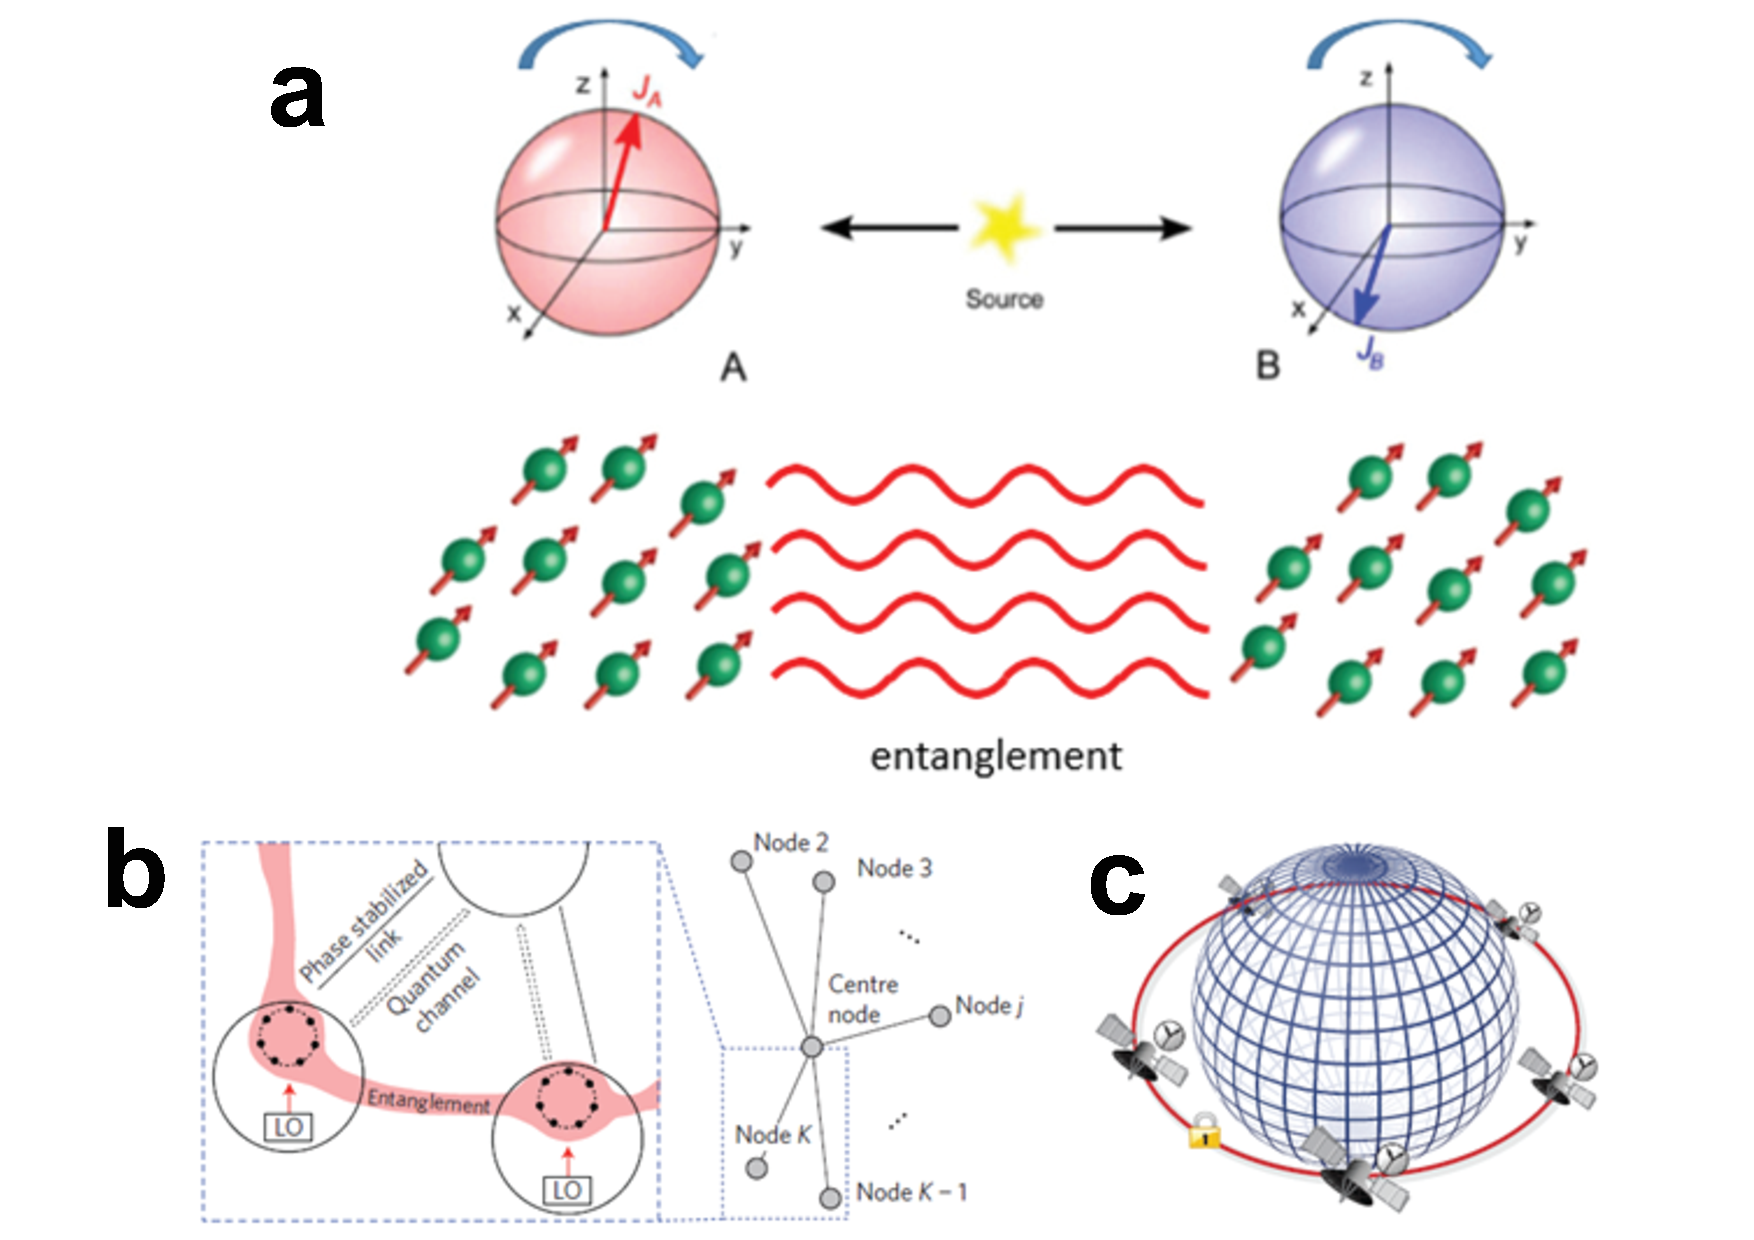
\includegraphics[clip=true, width=\textwidth]{space_3}
\captionspacefig \caption{Quantum clock synchronisation schemes. (top) The proposal by Jozsa \& Dowling \textit{et al.} where a singlet state\index{Bell states} is shared and measured in an ensemble of qubits \cite{bib:jozsa00}. (bottom) The proposal by Lukin \& Ye \textit{et al.} where a GHZ state\index{Greenberger-Horne-Zeilinger (GHZ) states} is distributed between satellites to measure the frequency drift at the Heisenberg limit \cite{bib:komar14}.}
\label{fig:space_3}
\end{figure*}

Previous works have examined the problem of clock synchronisation in space \comment{(see also Sec. [TB: refer to other section on clock sync])}. In the proposal of Jozsa \textit{et al.}, many copies of shared entanglement in a singlet state\index{Bell states} is first distributed and stored on the clock states of an atomic clock \cite{bib:jozsa00}. The measurement is then performed by one party, which collapses the states simultaneously across all parties, and the time evolution of the states begins.

Classical information is exchanged between them, which reveals the time elapsed since the measurement, which can be used to synchronise the clocks. While the original protocol only allowed clock synchronisation between two parties, similar ideas were used to extend this to the multiparty context \cite{bib:krvco2002quantum, bib:ben2011optimized, bib:ren2012clock}.

In a more recent proposal, a shared GHZ state\index{Greenberger-Horne-Zeilinger (GHZ) states} is prepared across all nodes in the quantum network, which allows for quantum metrologically enhanced detection\index{Quantum metrologically enhanced detection} of the clock signal drift at the Heisenberg limit\index{Heisenberg limit} \cite{bib:komar14}. The use of shared resources acts to improve the overall precision, allowing for an optimal scheme for the qubit resources that are employed. Several other proposals have also been made, which are quantum versions of Eddington's slow clock transport protocol\index{Eddington's slow clock transport protocol} where the qubit keeps time of the transmission \cite{bib:chuang2000quantum, bib:tavakoli2015quantum}. 

Experimentally, there have been several demonstrations of the protocol, albeit at relatively short distances. Continuous time-bin\index{Time-bin encoding} entangled photons were used as the entanglement resource to obtain a time-correlation between a distance of 3km \cite{bib:valencia2004distant}, and another technique based on Hong-Ou-Mandel interferometry\index{Hong-Ou-Mandel (HOM) interference} was performed across a 4km fibre link \cite{bib:quan2016demonstration}. Several other demonstrations based on nuclear magnetic resonance (NMR)\index{Nuclear magnetic resonance} \cite{bib:zhang2004nuclear, bib:kong2017implementation} have also been performed. 

There are however several outstanding problems with the quantum clock synchronisation scheme as presented above. In the scheme of Jozsa \textit{et al.}, if one starts in a perfect singlet state\index{Bell states}, the scheme works as intended, but if one instead starts with the state, 
\begin{align}
\frac{1}{\sqrt{2}} ( | 0 \rangle_A | 1 \rangle_B - e^{i \delta} | 1 \rangle_A | 0 \rangle_B ),
\end{align}
(a Bell pair augmented by a local phase) one obtains an offset to the synchronisations between the two parties. In practice, such a phase could arise from decoherence induced noise, or differences in the basis conventions chosen by the two parties. Thus, in practice entanglement purification\index{Entanglement purification} would be required to produce a singlet state with \mbox{$\delta=0$} prior to executing the protocol. However, it was argued that to perform the entanglement purification quantum circuit correctly, the timing of the quantum gates would need to be controlled, which requires synchronised clocks \cite{bib:preskill2000quantum} --  this renders synchronisation impossible. It has previously been shown that such a phase cannot be eliminated using asynchronous entanglement purification\index{Entanglement purification} \cite{bib:yurtsever02}, and hence the protocol remains incomplete in the general case where imperfect singlet pairs\index{Bell states} are shared.

\comment{Need to reference figure}

\comment{Peter's start - fix this}

A quantum protocol for clock synchronisation based on shared entanglement is given in Alg.~\ref{alg:clock_sync}.

\begin{table}[!htbp]
\begin{mdframed}[innertopmargin=3pt, innerbottommargin=3pt, nobreak]
\texttt{
function ClockSync($\ket{\Psi^-}$):
\begin{enumerate}
\item Distribute a Bell state between Alice and Bob,
\begin{align}
\ket{\psi_0} &= \frac{1}{\sqrt{2}}(\ket{0}_A\ket{1}_B - \ket{1}_A\ket{0}_B)\nonumber\\
	&= \frac{1}{\sqrt{2}}(\ket{+}_A\ket{-}_B - \ket{-}_A\ket{+}_B).
\end{align}
\item The joint system is freely-evolving under the Hamiltonian,
\begin{align}
\hat{H} = \hbar\omega(\hat{Z}_A + \hat{Z}_B).	
\end{align}
\item Over time $t_\mathrm{free}$ this evolves to,
\begin{align}
	\ket{\psi_1} &= e^{-i\frac{\hat{H}}{\hbar} t_\mathrm{free}}\frac{1}{\sqrt{2}}(\ket{+}_A\ket{-}_B - \ket{-}_A\ket{+}_B)\nonumber\\
	&= e^{-i\omega t_\mathrm{free}}\frac{1}{\sqrt{2}}(\ket{+}_A\ket{-}_B - \ket{-}_A\ket{+}_B),
\end{align}
yielding only an irrelevant global phase.
\item Alice measures her qubit in the $\hat{X}$ basis ($\ket\pm\bra\pm$), and classically announces the time at which she performed the measurement, $t_A$, and her measurement outcome, \mbox{$m_A=\pm$}.
\item The system evolves for time $t_\mathrm{ev}$,
\begin{align}
	\ket{\psi_{+}} &= e^{-i\hat{Z} t_\mathrm{ev}}\ket{-}_B\nonumber\\
	&\propto \ket{0}_B-e^{-i\omega t_\mathrm{ev}}\ket{1}_B,\nonumber\\
	\ket{\psi_{-}} &= e^{-i\hat{Z} t_\mathrm{ev}}\ket{+}_B\nonumber\\
	&\propto \ket{0}_B+e^{-i\omega t_\mathrm{ev}}\ket{1}_B.
\end{align}
\item Bob measures his qubit in the $\hat{X}$ basis, with measurement probabilities,
\begin{align}
	m_+ &\propto \sin^2(\omega t_\mathrm{ev}),\nonumber\\
	m_- &\propto \cos^2(\omega t_\mathrm{ev}),
\end{align}
and infers $t_\mathrm{ev}$.
\item Bob sets his clock to,
\begin{align}
	t_B = t_A+t_\mathrm{ev}.
\end{align}
\item $\Box$
\end{enumerate}
}
\end{mdframed}
\captionspacealg \caption{Algorithm for performing quantum clock synchronisation between two parties using shared Bell-pairs and classical communication.\comment{Check this for errors!}} \label{alg:clock_sync}
\end{table}

%
% Quantum-Enabled Telescopy
%

\subsection{Quantum-enabled telescopy}\index{Quantum-enabled telescopy}\label{sec:telescopy}

For the direct imaging of an object, diffraction limits the resolution of the image. When we consider two neighbouring points on the object separated by a small angle, the minimum angular separation resolvable is,
\begin{align}
	\theta_\mathrm{min} = 1.22 \frac{\lambda}{D},
\end{align}
known as the Rayleigh criterion\index{Rayleigh criterion}, $D$ being the diameter of the aperture\index{Aperture}.

Current optical interferometers have limited baseline lengths\index{Baseline length}, and thus limited resolution. In principle one can build a telescope array with a synthetic aperture\index{Synthetic aperture} of arbitrary $D$, however, phase-locking the entire system is extremely difficult over long distances. A quantum information protocol has been developed to side-step this problem.

The light arriving from the distant object is a thermal state, but the average photon number per mode is much less than 1, therefore higher order terms are negligible. The state that reaches the telescope is therefore approximated by,
\begin{align}
\ket{\psi_\mathrm{image}} = \frac{1}{\sqrt{2}}(\ket{0}_A\ket{1}_B + e^{i\phi}\ket{1}_A\ket{0}_B),
\end{align}
where $\phi$ is the relative phase-shift between the two telescopes, which depends on the difference in distance of propagation. If $\phi$ can be measured accurately, this can give a precise estimate on the location of the object,
\begin{align}
\phi = \frac{b \sin(\theta)}{\lambda},
\end{align}
where $\lambda$ is wavelength.

Often the light that arrives will be formed by a mixture of photons from different sources that emit incoherently, and different locations give rise to different phase-shifts $\phi$, resulting in a density matrix of the form,
\begin{align}
\hat\rho = \frac{1}{2} \left(\begin{matrix}{}
  0 & 0 & 0 & 0 \\
  0 & 1 & \mathcal{V}^* & 0 \\
  0 & \mathcal{V} & 1 & 0 \\
  0 & 0 & 0 & 0
\end{matrix}\right),
\end{align}
where $\mathcal{V}$ is the visibility, reflecting decoherence.

If we interfere the two modes at a 50:50 beamsplitter, the photon will exit port 1 with probability,
\begin{align}
	p_\mathrm{coin} = \frac{1}{2} (1 + \mathrm{Re}[\mathcal{V}e^{-i\delta}]),
\end{align}
from which $\mathcal{V}$ can be determined by taking measurements while sweeping through $\delta$.

The problem with implementing the measurement is the difficulty of transporting the single photon state over long distances without incurring loss or additional phase-shifts.

Instead of sending a valuable quantum state directly over a noisy quantum channel, one can distribute a Bell pair between the two telescopes, then we teleport the original quantum state from one telescope to the other. The entangled state is known, the preparation can be repeated, and one can use an entanglement distillation protocol to eliminate the phase noise.

Now, we can use the entangled pair directly to measure the visibility, as in Fig.~\ref{fig:telescopy}. We post-select on the measurement results, considering the events where a single photon is observed at $A$ and $B$ simultaneously.

\begin{figure}[!htbp]
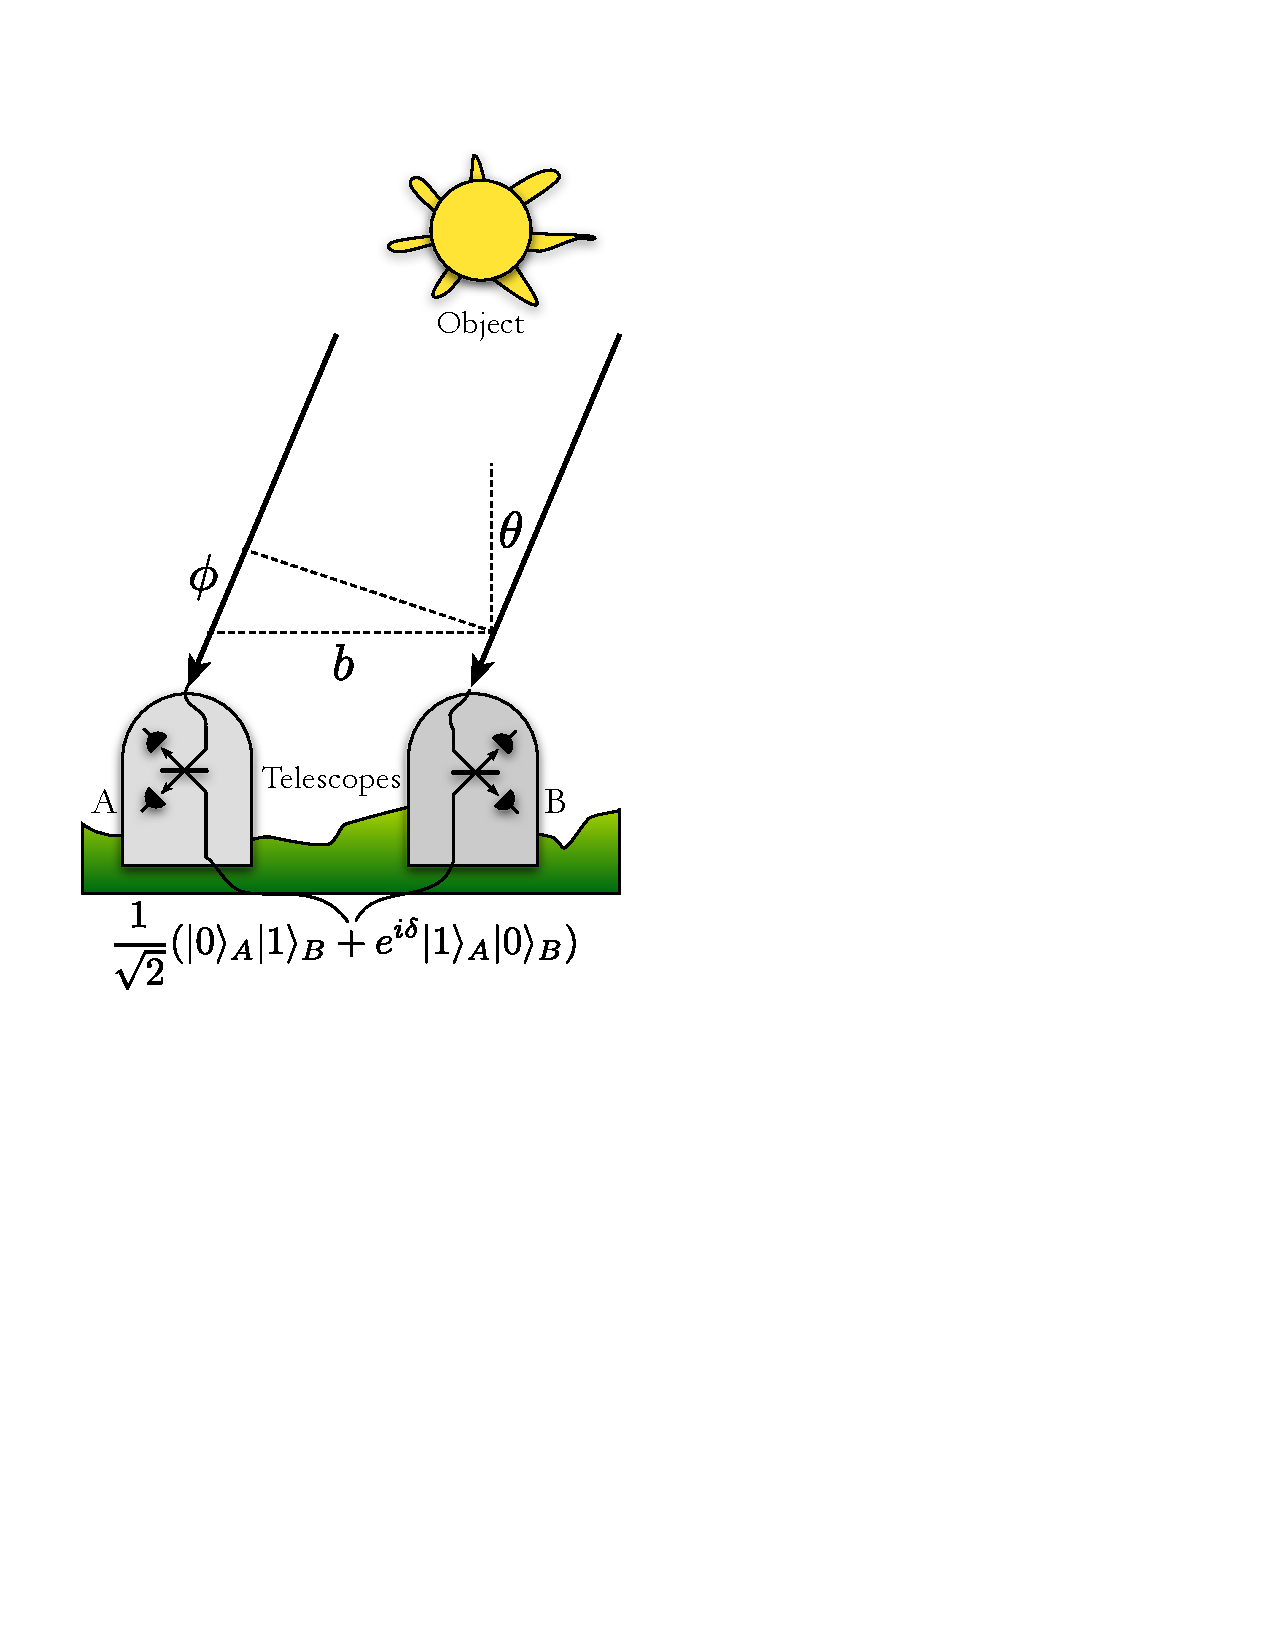
\includegraphics[clip=true, width=0.4\textwidth]{telescopy}
\captionspacefig \caption{Architecture for quantum-enabled telescopy using two widely separated telescopes, which have shared Bell pairs. The basic idea is that the Bell pair mediates teleportation of one telescope's photon to the other, at which point an interferometric technique measures their phase-difference, thereby determining $\phi$.}\label{fig:telescopy}\index{Quantum-enabled telescopy}	
\end{figure}

The variable delay line is now applied to the entangled state when the photon is sent to $A$, producing the entangled state,
\begin{align}
\ket{\psi_\mathrm{shared}} = \frac{1}{\sqrt{2}}(\ket{0}_A\ket{1}_B + e^{i\delta}\ket{1}_A\ket{0}_B),	
\end{align}
where $\delta$ is determined by a controllable delay, allowing completion of the protocol to determine $\phi$.

Thinking futuristically, in a future large-scale quantum internet, whereby Bell pairs are a readily available resource across the globe, quantum-enabled telescopy needn't be limited to pairs of telescopes, but could expand to become large-scale telescope arrays\index{Telescope arrays} comprising numerous telescopes, all sharing pairwise entanglement, distributed via the quantum internet (see Fig.~\ref{fig:telescope_array}). Using a 2D grid would enable $\theta$ to be measured along different axes, and the increased number of detectors would increase signal strength.

\begin{figure}[!htbp]
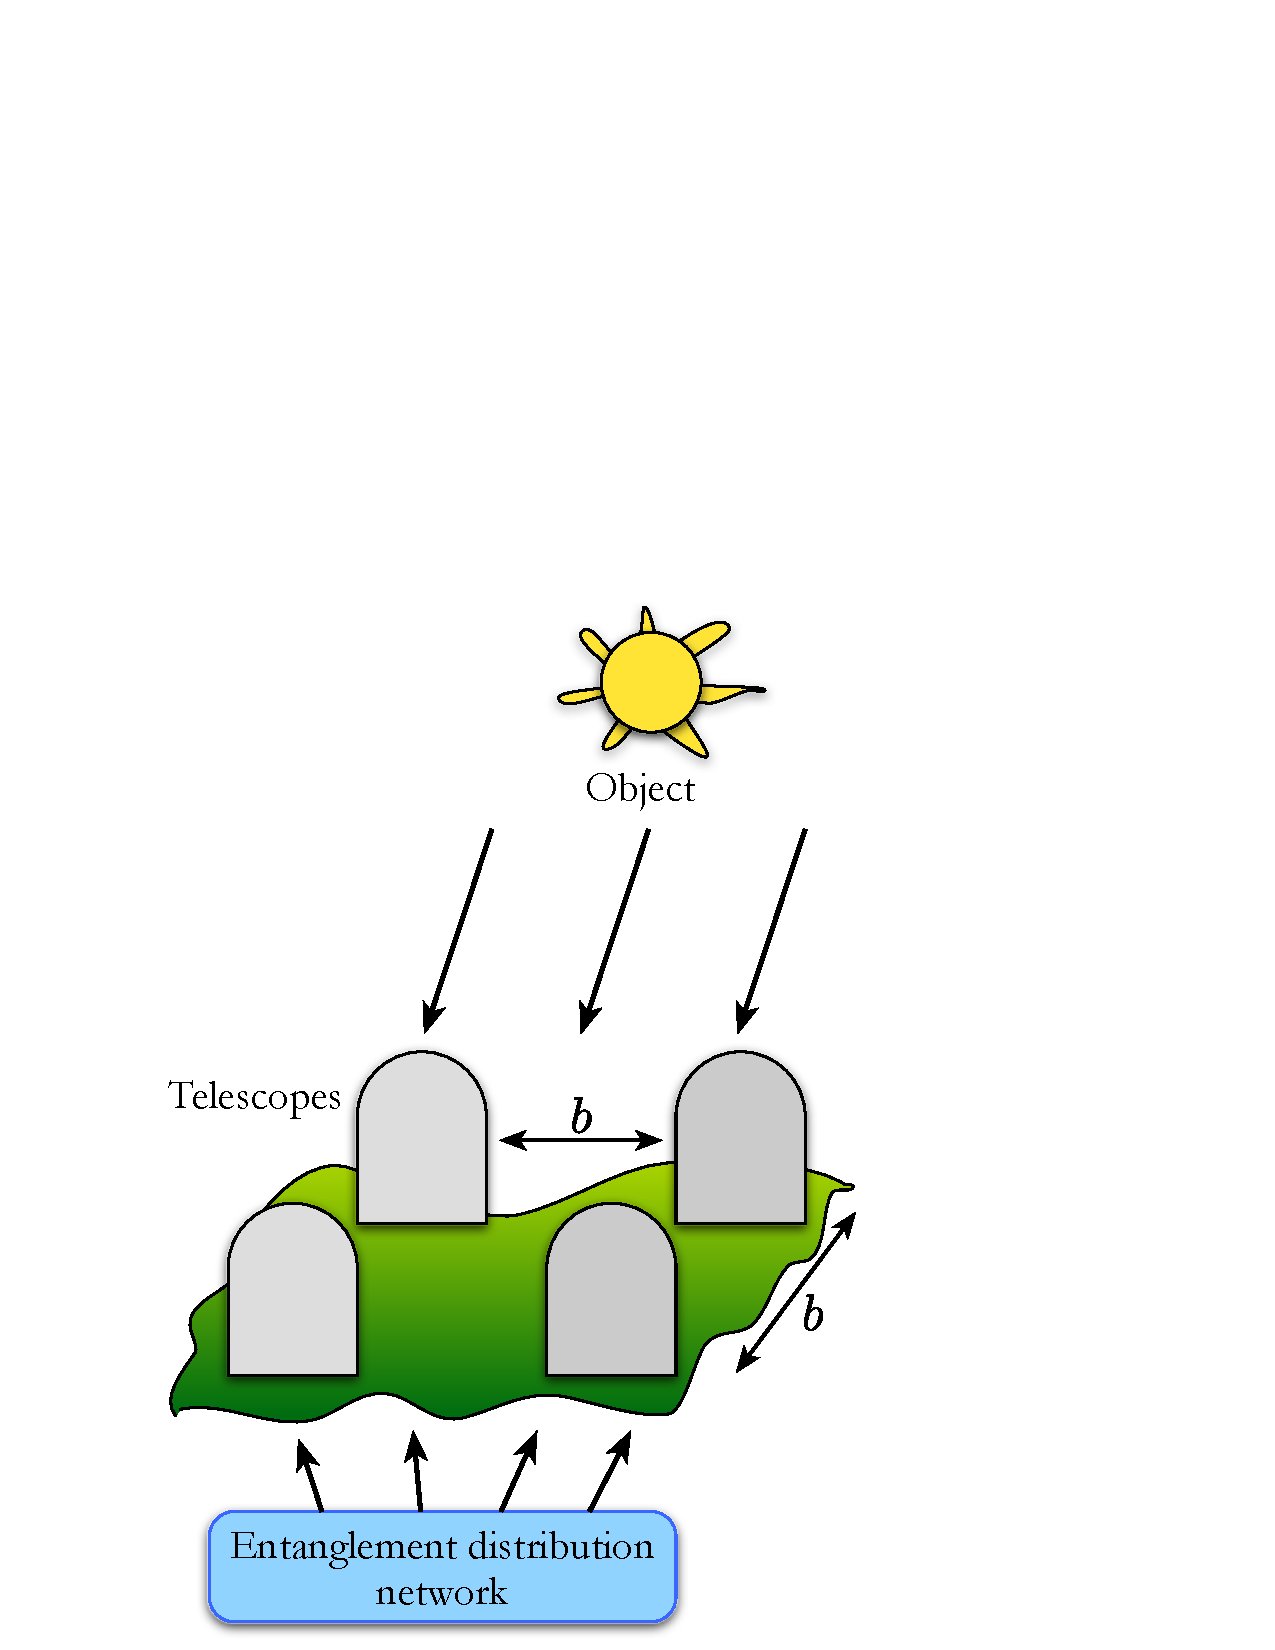
\includegraphics[clip=true, width=0.475\textwidth]{telescope_array}
	\captionspacefig \caption{An array of quantum-enabled telescopes, paired with one another via Bell-pairs, distributed over a quantum network. With more telescopes in the array, signal strength can be increased, and if the array has a 2D grid topology, rather than a linear one, the angles of incident light fields can be measured along multiple axes.}\label{fig:telescope_array}\index{Telescope arrays}
\end{figure}

 %The total probability of seeing a correlation ($A1$, $B1$ or $A2$, $B2$), conditioned on having one click at each telescope is,
%\begin{align}
% 	frac{1}{2} (1 + \mathrm{Re}[\mathcal{V}e^{-i\delta}]),
%\end{align}
%and the total probability of seeing an anti-correlation ($A1$, $B2$ or $A2$, $B1$) is \cite{bib:PhysRevLett.109.070503},
%\begin{align}
%	\frac{1}{2} (1 - \mathrm{Re}[\mathcal{V}e^{-i\delta}]).
%\end{align}